\documentclass[twoside,notitlepage,11pt]{report}
%\usepackage{a4paper}
\usepackage{graphicx}
\usepackage{psfrag}
\usepackage{amsfonts}
\usepackage{amsmath}
\usepackage{amsbsy}
\usepackage{verbatimfile}
\usepackage{fancyhdr}
\usepackage{pstricks,pst-node}
% The next rawfonts package one is used in the ``datablad''.
\usepackage[only,egtrm]{rawfonts}
% Handle sorting in reference list
\usepackage{citesort}
% Create an index table
\usepackage{makeidx}

\newcommand{\smallverbatimfile}[1]{{\footnotesize\verbatimfile{#1}}}
\newcommand{\component}[5]{\begin{tabular}{|lp{0.7\textwidth}|}\hline {\bf Name:} & #1 \\ \hline {\bf Author:} & #2 \\ \hline {\bf Input parameters} & #3 \\ \hline {\bf Optional parameters} & #4 \\ \hline {\bf Notes} & #5 \\ \hline \end{tabular} \\ \noindent }

\def\reportnum{Ris{\o}--R--1xyz(EN)}

%\oddsidemargin 0cm
%\evensidemargin 0cm
\addtolength{\hoffset}{-1.4cm}
\topmargin 0cm
\textwidth 15cm
\textheight 22cm
\addtolength{\footskip}{1.6pt}
\addtolength{\headheight}{1.6pt}

\pagestyle{fancy}
\fancyhf{}
\fancyfoot[LE,RO]{\thepage}
\fancyfoot[LO,RE]{\reportnum}
\renewcommand{\headrulewidth}{0pt}
\renewcommand{\footrulewidth}{0pt}

\fancypagestyle{plain}{%
\fancyhf{}
\fancyfoot[LE,RO]{\thepage}
\fancyfoot[RE,LO]{\reportnum}
\renewcommand{\headrulewidth}{0pt}
\renewcommand{\footrulewidth}{0pt}}

\newcommand{\MCS}{{McStas}}
\newcommand{\version}{{1.9}}
\newcommand{\reldate}{{October 31, 2005}}
\newcommand{\Ombold}{\mbox{\boldmath $\Omega$}}

% enable index generation
\makeindex

%\title{Component manual\\ to the neutron ray-tracing package
% \MCS ,\\ version \version}
%\author{Kim Lefmann, Peter Kj\ae r Willendrup, and Kristian Nielsen, \\
% Materials Research Department, \\
% Ris\o\ National Laboratory, 4000 Roskilde, Denmark;\\
% Emmanuel Farhi and Klaus Lieutenant \\ ILL, Grenoble, France}
%\date{\reldate \\[2\baselineskip]
%\begin{center}
%  \includegraphics[width=4.5in]{figures/vanadium-surf-2.eps}
%\end{center}
%
\includegraphics[width=0.45\myheight]{risoe-logo.eps}%
%}
\begin{document}

%\maketitle
% Emacs settings: -*-mode: latex; TeX-master: "manual.tex"; -*-

\begingroup                     % Make all definitions local.

%
% This was modified from risoe.sty, <2 Aug 95>
%
\catcode`\@=11
\def\@magscale#1{ scaled \magstep#1 }
\font\frtnbf = cmb10 \@magscale2
\font\twfvbf = cmbx10   \@magscale5 % extended bold
\def\maketitle{\par
 \begingroup
 \def\thefootnote{\fnsymbol{footnote}}
 \def\@makefnmark{\hbox to 0pt{$^{\@thefnmark}$\hss}}
 \if@twocolumn
 \twocolumn[\@maketitle]
 \else \newpage
 \global\@topnum\z@ \@maketitle \fi\thispagestyle{empty}\@thanks\newpage
 \endgroup
 \setcounter{footnote}{0}
 \let\maketitle\relax
 \let\@maketitle\relax
 \gdef\@thanks{}\gdef\@author{}\gdef\@title{}\let\thanks\relax}
\def\@maketitle{\newpage \baselineskip 30dd \mbox{}
 \marginpar{{\frtnbf \hfill \llap{\mbox{\reportnum \reportlan\qquad\qquad}}}}
 \par\noindent\mbox{
\includegraphics[height=1.5cm]{figures/risoe-logo.eps}\hspace{2mm}
\includegraphics[height=1.5cm]{figures/DTU_logo.ps}} \par
 \vskip 1.5cm
 {\twfvbf \noindent \@title \par} \vskip 20dd \baselineskip 16dd
 {\frtnbf\noindent\@author \par} 
 \vskip 0.5cm
 \begin{center}
     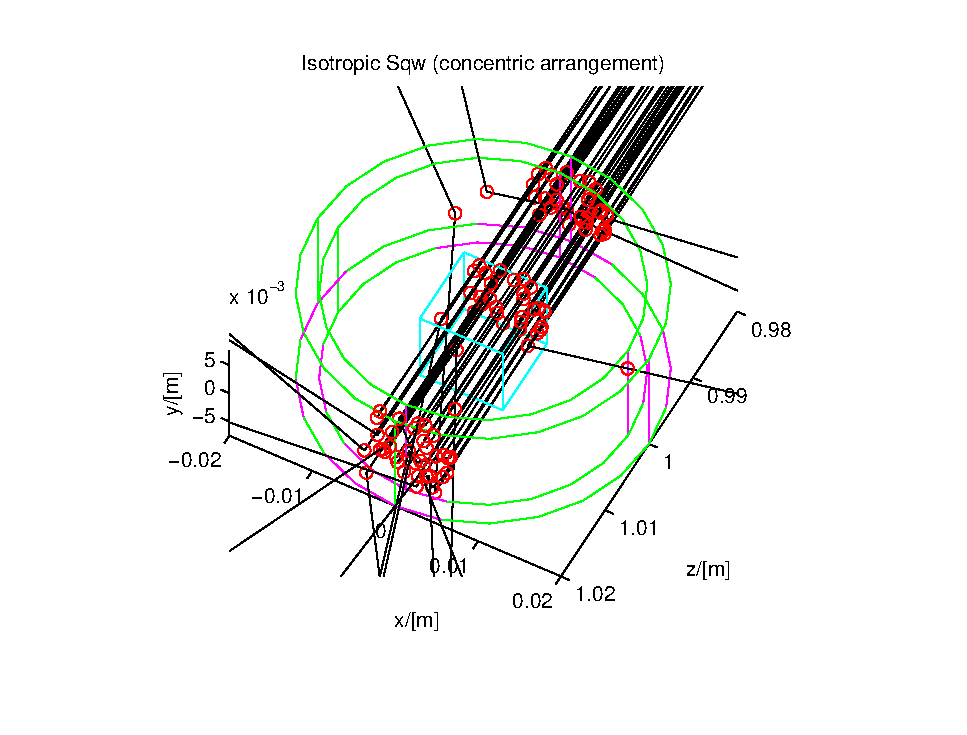
\includegraphics[width=\textwidth]{figures/sqw.eps}
   \end{center}
   \par \vfill \baselineskip 12dd
 \frtnbf\noindent Ris{\o} DTU, Roskilde, Denmark \par
 \vskip 4dd \noindent\ifcase\month\or
 January\or February\or March\or April\or May\or June\or
 July\or August\or September\or October\or November\or December\fi
 \space\number\year }

\let\reportlan=\relax
\def\month{5}                   % Released in November 2005
% Need to match front page line breaking.
\title{Component~Manual~for~\rlap{the}\\ % Avoid overfull message.
 X-Ray-Tracing~Package\\
 \MCX, Version \version\ }
\author{Peter Kj\ae r Willendrup, Erik Knudsen, Kim Lefmann and\\Emmanuel Farhi}
\maketitle
\endgroup

%\begin{center}
%  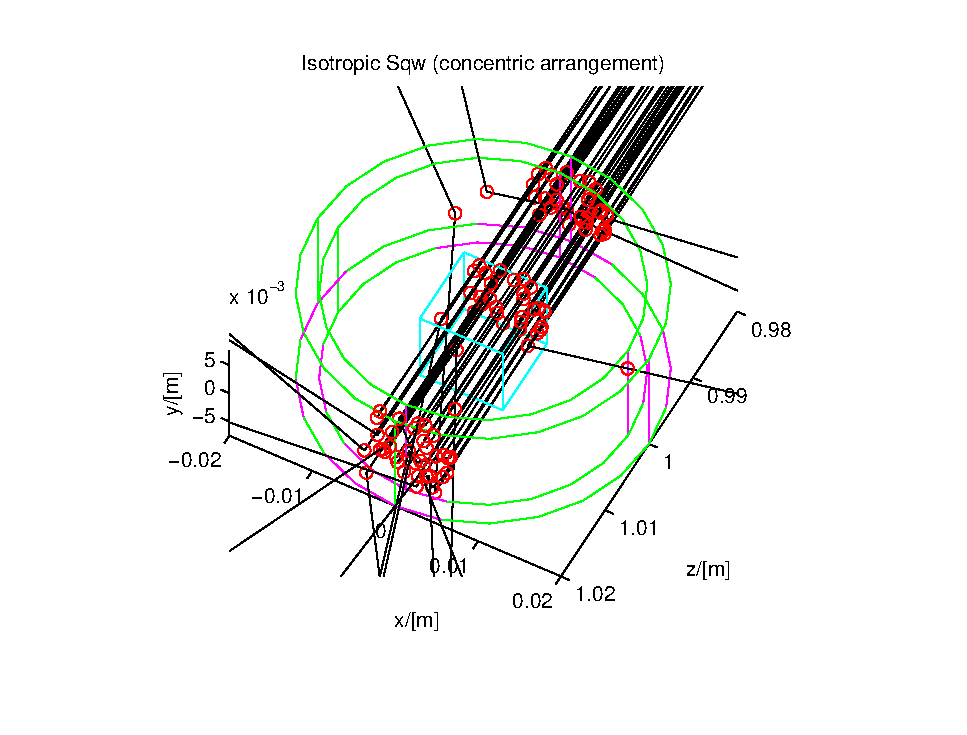
\includegraphics[width=4.5in]{figures/sqw.eps}
%\end{center}
%
% NOTE: Find a way to include this nice graphics on front page
% Currently this does not work?!?

\thispagestyle{empty}
% Emacs settings: -*-mode: latex; TeX-master: "manual.tex"; -*-

\begin{abstract}
The software package McStas is a tool for carrying out Monte Carlo
ray-tracing simulations of neutron scattering instruments with high
complexity and precision. The simulations can compute most aspects of the
performance of instruments and samples
and can thus be used to optimize the use of existing equipment,
design new instrumentation, and carry out full virtual experiments.
McStas is based on a unique design where an automatic compilation process
translates high-level textual instrument descriptions into efficient
ANSI-C code. This design makes it simple to set up typical simulations
and also gives essentially unlimited freedom to handle more unusual
cases.

This report constitutes the component manual for McStas, and,
together with the manual for the McStas system, it
contains full documentation of all aspects of the program. It covers
a description of all official components of the \MCS\ package with
some theoretical background. Selected test
instruments and representative \MCS\ simulations performed with these
instruments are described in the User Manual.


\end{abstract}

\vskip\baselineskip\noindent
This report documents the components for McStas version \version,
released \reldate .
\vskip\baselineskip\noindent
The authors are:
\begin{quote}
\label{p:authors}
\vskip\baselineskip\noindent
Kim Lefmann \\
Materials Research Department, Ris{\o} National Laboratory, Roskilde, Denmark \\
email: \verb+kim.lefmann@risoe.dk+
\vskip\baselineskip\noindent
Peter Kj\ae r Willendrup \\
Materials Research Department, Ris{\o} National Laboratory, Roskilde, Denmark \\
email: \verb+peter.willendrup@risoe.dk+
\vskip\baselineskip\noindent
Kristian Nielsen \\
email: \verb+kristian.nielsen@mail.tele.dk+
\vskip\baselineskip\noindent
Emmanuel Farhi \\
Institut Laue-Langevin, Grenoble, France \\
email: \verb+farhi@ill.fr+
\vskip\baselineskip\noindent
Klaus Lieutenant \\
Institut Laue-Langevin, Grenoble, France \\
email: \verb+lieutenant@ill.fr+
\end{quote}
%Front page illustration:\\[\baselineskip]
%Simulated scattering from a vanadium sample
%taking into account the secondary extinction. See
%section~\ref{s:vanadium-result}.
\vfill
\noindent ISBN 87--550--3482--9
\par\noindent ISSN 0106--2840
\par\noindent\hbox{}\hfill
    Pitney Bowes Management Services Denmark A/S $\cdot$ Ris{\o} National Laboratory $\cdot$ \number\year
%    Information Service Department $\cdot$ Ris{\o} $\cdot$ \number\year
\par
\thispagestyle{empty}\clearpage


\tableofcontents
%\pagebreak
%\listoffigures
%\pagebreak
%\listoftables

% Emacs settings: -*-mode: latex; TeX-master: "manual.tex"; -*-

\addcontentsline{toc}{chapter}{\protect\numberline{}{Preface and acknowledgements}}
\chapter*{Preface and acknowledgements}
This document contains information on the neutron scattering components 
which are the building blocks for describing instruments 
in the Monte Carlo neutron
ray-tracing program \MCS\ version \version . The initial
release in October 1998 of version 1.0 was presented in Ref.~\cite{NNews}. 
The reader of this
document is not supposed to have specific knowledge of neutron scattering,
but some basic understanding of the underlying physics is helpful in
understanding the theoretical background for the component functionality. 
For details about simulation techniques, we refer to 
the \MCS\ system manual \cite{mcstasmanual}.
We assume familiarity with the use of 
the C programming language.

We especially like to thank Kristian Nielsen for laying a solid foundation
for the \MCS\ system, which the authors of this manual benefit from daily.
Also Per-Olof \AA strand has contributed to the development of
the \MCS\ system.
It is a pleasure to thank Dir.~Kurt N.~Clausen for his continuous
support to \MCS\ and for having initiated the project.
Continuous support to \MCS\ has also come from Prof.~Robert McGreevy.
%Both he and our other collaborators, Henrik M.\ R\o nnow and Mark
%Hagen have made major contributions to the project.  Also the
%contributions from our test users, the students Asger Abrahamsen, Niels
%Bech Christensen, and Erik Lauridsen, are gratefully acknowledged; they
%gave us an excellent opportunity to pinpoint a vast amount of serious
%errors in the test version.  Useful comments to this document itself
%have been given by Bella Lake and Alan Tennant.  
We have further benefited
from discussions with many other people in the neutron scattering
community, too numerous to mention here.

%Philipp Bernhardt contributed the two chopper components in
%sections~\ref{s:chopper} and~\ref{s:first_chopper}. Emmanuel Farhi
%contributed the components in sections~\ref{s:sourceoptimizer},
%\ref{s:monitornd}, and~\ref{s:monitoroptimizer}. 
The users who contributed components to this manual are acknowledged
as authors of the individual components. We encourage other
users to contribute components with manual entries for inclusion in
future versions of \MCS.

In case of any errors, questions, suggestions, 
%or other need for support should arise,
do not hesitate to 
contact the authors at \verb+mcstas@risoe.dk+
or consult the \MCS\ WWW home page~\cite{mcstas_webpage}.

Important developments on the component side in \MCS\ version \version\ 
as compared to version 1.4 (the last version of the component manual) include

\begin{itemize}
\item ... so much that I do not know what to say...
\end{itemize} 

The \MCS\ project has been supported by the European Union, initially
through the XENNI program and the RTD ``Cool Neutrons'' program in FP4,
In FP5, \MCS\ was supported strongly through the
``SCANS'' program. 
Currently, in FP6, \MCS\ is supported through the Joint Research Activity
``MCNSI'' under the Integrated Infrastructure Initiative ``NMI3'', see
the WWW home pages~\cite{mcnsi_webpage,nmi3_webpage}







% Emacs settings: -*-mode: latex; TeX-master: "manual.tex"; -*-

\chapter{About the component library}
\label{c:components}
This \MCX\ Component Manual consists of the following major parts:
\begin{itemize}
\item An introduction to the use of Monte Carlo methods in \MCX .
\item A thorough description of system components,
with one chapter per major category: Sources, optics,
monochromators, samples, monitors, and other components.
\item The \MCS\ library functions and definitions
  that aid in the writing of simulations and components in
  Appendix~\ref{c:kernelcalls}.
%\item A detailed explanation of the use of random numbers
%   in Appendix~\ref{s:random}.
\item An explanation of the \MCX\ terminology in Appendix~\ref{s:terminology}.
\end{itemize}
Additionally, you may refer to the list of example instruments
from the library in the \MCX\ User Manual.

\section{Authorship}
The component library is
maintained by the \MCX\ system group. A number of basic components
``belongs'' the \MCX\ system, and are supported and tested by the \MCX\
team.

Other components are contributed
by specific authors, who are listed in the code for each component
they contribute as well as in this manual.
\MCS\ users are encouraged to send their
contributions to us for inclusion in future releases.

%Some contributed components have later been taken over
%for further development by the \MCX\ system
%group, with permission from the original authors.
%The original authors will still appear both in the component code and in the
%\MCS\ manual.

\section{Symbols for neutron scattering and simulation}
In the description of the theory behind the component functionality
we will use the usual symbols {\bf r} for the position
$(x,y,z)$ of the particle (unit m), and {\bf v} for
the particle velocity $(v_x, v_y, v_z)$ (unit m/s).
Another essential quantity is the neutron wave vector
${\bf k} = m_{\rm n} {\bf v}/\hbar$ , where
$m_{\rm n}$ is the neutron mass. {\bf k} is usually given in
\AA$^{-1}$, while neutron energies are given in meV.
The neutron wavelength is the reciprocal wave vector,
$\lambda=2 \pi / k$.
In general, vectors are denoted by boldface symbols.

Subscripts "i" and "f" denotes ``initial'' and ``final'', respectively,
and are used in connection with the neutron state before and after
an interaction with the component in question.
%This is of particular importance in sample components, where the
%wave vector change is denoted the {\em scattering vector}
%\begin{equation}\label{eq:q-transfert}
%{\bf q} \equiv {\bf k}_{\rm i} - {\bf k}_{\rm f} .
%\end{equation}
%In analogy, the {\em energy transfer} is given by
%\begin{equation}\label{eq:w-transfert}
%\hbar \omega \equiv E_{\rm i}-E_{\rm f} =
%\frac{\hbar^2}{2 m_{\rm n}} \left( k_{\rm i}^2 - k_{\rm f}^2 \right).
%\end{equation}


\section{Component coordinate system}
All mentioning of component geometry refer to
the local coordinate system of the individual component.
The axis convention is so that the $z$ axis is along
the neutron propagation axis, the $y$ axis is vertical up,
and the $x$ axis points left when looking along the $z$-axis,
completing a right-handed coordinate system.
Most components 'position' (as specified in the instrument description
with the \verb+AT+ keyword) corresponds to their input side at the nominal
beam position.
However, a few components are radial and thus positioned in their centre.
\index{Symbols}\index{Coordinate system}

Components are not necessarily designed to overlap.
This may lead to loss of rays.
Warnings will be issued during simulation if sections of the instrument
are not reached by any xrays, or if a significant number of xrays are removed.
This is usually the sign of either overlapping components
or a very low intensity.\index{Removed xray events}

\section{About data files}\index{Data files}\index{Library!read\_table-lib (Read\_Table)}
Some components require external data files,
e.g. lattice crystallographic definitions for Laue and powder pattern diffraction,
$S(q,\omega)$ tables for inelastic scattering,
absoprtion and reflectivity files, etc.

Such files distributed with \MCX\ are located in the
\verb+data+ sub-directory of the \verb+MCXTRACE+ library.
Components that make use of the \MCX\ file system,
including the \verb+read-table+ library (see section \ref{s:read-table})
may access all \MCX\ data files without making local copies.
Of course, you are welcome to define your own data files,
and eventually contribute to \MCX\ if you find them useful.

File extensions are not compulsory but help in identifying relevant files per
application. We list powder and liquid data files from the \MCS\ library in
Tables \ref{t:powders-data} and \ref{t:liquids-data}. These files contain an
extensive header describing physical properties with references, and are
specially suited for the PowderN (see \ref{powder}) and Isotropic\_Sqw
components (see \ref{s:isotropic-sqw}).

\begin{table}
  \begin{center}
    {\let\my=\\
    \begin{tabular}{|p{0.24\textwidth}|p{0.7\textwidth}|}
      \hline
       {\bf MCSTAS/data} & Description \\
       \hline
 *.lau & Laue pattern file, as issued from Crystallographica.
       For use with Single\_crystal, PowderN, and Isotropic\_Sqw.
       Data: [ h   k   l Mult. d-space 2Theta   F-squared ] \\
 *.laz & Powder pattern file, as obtained from Lazy/ICSD.
       For use with PowderN, Isotropic\_Sqw and possibly Single\_crystal.\\
 *.trm & transmission file, typically for monochromator crystals and filters.
       Data: [ k (Angs-1) , Transmission (0-1) ] \\
 *.rfl & reflectivity file, typically for mirrors and monochromator crystals.
       Data: [ k (Angs-1) , Reflectivity (0-1) ] \\
 *.sqw & $S(q,\omega)$ files for Isotropic\_Sqw component.
       Data: [q] [$\omega$] [$S(q,\omega)$]\\
      \hline
    \end{tabular}
    \caption{Data files of the \MCS\ library.}
    \label{t:comp-data}
    \index{Library!Components!data}
    }
  \end{center}
\end{table}

\begin{table}
  \begin{center}
    {\let\my=\\
    \begin{small}
    \begin{tabular}{|l|rrr|rr|p{0.2\textwidth}|}

      \hline
      {\bf MCSTAS/data} & $\sigma_{coh}$&$\sigma_{inc}$&$\sigma_{abs}$&$T_m$       & $c$    & Note \\
          File name     & [barns]     & [barns]    & [barns]    & [K]        & [m/s] & \\
      \hline
Ag.laz             & 4.407     & 0.58     &{\bf 63.3}      &1234.9    &2600&\\
Al2O3\_sapphire.laz & 15.683    & 0.0188   &0.4625    &2273      &   &\\
Al.laz             & 1.495     & 0.0082   &0.231     &933.5     &5100& .lau\\
Au.laz             & 7.32      & 0.43     &{\bf 98.65}     &1337.4    &{\bf 1740}&\\
B4C.laz            & 19.71     & 6.801    &{\bf 3068}      &2718      &     &\\
Ba.laz             & 3.23      & 0.15     &29.0      &1000      &{\bf 1620}&\\
Be.laz             & 7.63      & 0.0018   &0.0076    &1560      &13000&\\
BeO.laz            & 11.85     & 0.003    &0.008     &2650      &   & .lau\\
Bi.laz             & 9.148     & 0.0084   &0.0338    &544.5     &{\bf 1790}&\\
C60.lau            & 5.551     & 0.001    &0.0035    &          &   &\\
C\_diamond.laz      & 5.551     & 0.001    &0.0035    &4400      &18350 & .lau\\
C\_graphite.laz     & 5.551     & 0.001    &0.0035    &3800      &18350 & .lau\\
Cd.laz             & 3.04      & 3.46     &{\bf 2520}      &594.2     &2310&\\
Cr.laz             & 1.660     & 1.83     &3.05      &2180      &5940&\\
Cs.laz             & 3.69      & 0.21     &29.0      &301.6     &{\bf 1090}  & $c$ in liquid\\
Cu.laz             & 7.485     & 0.55     &3.78      &1357.8    &3570&\\
Fe.laz             & 11.22     & 0.4      &2.56      &1811      &4910&\\
Ga.laz             & 6.675     & 0.16     &2.75      &302.91    &2740&\\
Gd.laz             & 29.3      & 151      &{\bf 49700}     &1585      &2680&\\
Ge.laz             & 8.42      & 0.18     &2.2       &1211.4    &5400  & \\
H2O\_ice\_1h.laz     & 7.75      & 160.52   &0.6652    &273       &     &\\
Hg.laz             & 20.24     & 6.6      &{\bf 372.3}     &234.32    &{\bf 1407}&\\
I2.laz             & 7.0       & 0.62     &12.3      &386.85    &   &\\
In.laz             & 2.08      & 0.54     &{\bf 193.8}     &429.75    &{\bf 1215}&\\
K.laz              & .69       & 0.27     &2.1       &336.53    &{\bf 2000}&\\
LiF.laz            & 4.46      & 0.921    &{\bf 70.51}     &1140      &   &\\
Li.laz             & 0.454     & 0.92     &{\bf 70.5}      &453.69    &6000&\\
Nb.laz             & 8.57      & 0.0024   &1.15      &2750      &3480&\\
Ni.laz             & 13.3      & 5.2      &4.49      &1728      &4970&\\
Pb.laz             & 11.115    & 0.003    &0.171     &600.61    &{\bf 1260}&\\
Pd.laz             & 4.39      & 0.093    &6.9       &1828.05   &3070&\\
Pt.laz             & 11.58     & 0.13     &10.3      &2041.4    &2680&\\
Rb.laz             & 6.32      & 0.5      &0.38      &312.46    &{\bf 1300}  & \\
Se\_alpha.laz       & 7.98      & 0.32     &11.7      &494       &3350&\\
Se\_beta.laz        & 7.98      & 0.32     &11.7      &494       &3350&\\
Si.laz             & 2.163     & 0.004    &0.171     &1687      &2200&\\
SiO2\_quartza.laz   & 10.625    & 0.0056   &0.1714    &846       &      & .lau\\
SiO2\_quartzb.laz   & 10.625    & 0.0056   &0.1714    &1140      &      & .lau\\
Sn\_alpha.laz       & 4.871     & 0.022    &0.626     &505.08    &     &\\
Sn\_beta.laz        & 4.871     & 0.022    &0.626     &505.08    &2500&\\
Ti.laz             & 1.485     & 2.87     &6.09      &1941      &4140&\\
Tl.laz             & 9.678     & 0.21     &3.43      &577       &{\bf 818}&\\
V.laz              & .0184     & 4.935    &5.08      &2183      &4560&\\
Zn.laz             & 4.054     & 0.077    &1.11      &692.68    &3700&\\
Zr.laz             & 6.44      & 0.02     &0.185     &2128      &3800&\\
      \hline
    \end{tabular}\end{small}
    \caption{Powders of the \MCS\ library \cite{icsd_ill,ILLblue}. Low $c$ and high $\sigma_{abs}$ materials are highlighted. Files are given in LAZY format, but may exist as well in Crystallographica {\it .lau} format as well.}
    \label{t:powders-data}
    \index{Library!Components!data}
    }
  \end{center}
\end{table}

\begin{table}
  \begin{center}
    {\let\my=\\
    \begin{small}
    \begin{tabular}{|l|rrr|rr|p{0.2\textwidth}|}

      \hline
      {\bf MCSTAS/data} & $\sigma_{coh}$&$\sigma_{inc}$&$\sigma_{abs}$&$T_m$       & $c$    & Note \\
          File name     & [barns]     & [barns]    & [barns]    & [K]        & [m/s] & \\
      \hline
Cs\_liq\_tot.sqw                      & 3.69      & 0.21     &29.0      &301.6     &{\bf 1090}  & Measured \\
Ge\_liq\_coh.sqw and Ge\_liq\_inc.sqw & 8.42      & 0.18     &2.2       &1211.4    &5400  & Ab-initio MD \\
He4\_liq\_coh.sqw                     & 1.34      & 0        &0.00747   &0         &{\bf 240}   & Measured\\
Ne\_liq\_tot.sqw                      & 2.62      & 0.008    &0.039     &24.56     &{\bf 591}   & Measured\\
Rb\_liq\_coh.sqw and Rb\_liq\_inc.sqw & 6.32      & 0.5      &0.38      &312.46    &{\bf 1300}  & Classical MD \\
Rb\_liq\_tot.sqw                      & 6.32      & 0.5      &0.38      &312.46    &{\bf 1300}  & Measured \\
      \hline
    \end{tabular}\end{small}
    \caption{Liquids of the \MCS\ library \cite{icsd_ill,ILLblue}. Low $c$ and high $\sigma_{abs}$ materials are highlighted.}
    \label{t:liquids-data}
    \index{Library!Components!data}
    }
  \end{center}
\end{table}

\MCS\ itself generates both simulation and monitor data files, which structure is explained in the User Manual (see end of chapter 'Running \MCS\ ').

\section{Component source code}
Source code for all components may be found in the \verb+MCSTAS+ library
subdirectory of the McStas installation;
the default is \verb+/usr/local/lib/mcstas/+
on Unix-like systems and \verb+C:\mcstas\lib+ on Windows systems, but it may be
changed using the \verb+MCSTAS+ environment variable.
\index{Environment variable!MCSTAS}

In case users only require to add new features, preserving the existing features of a component, 
using the \verb+EXTEND+ keyword\index{Keyword!EXTEND} in the instrument description file is recommended. For larger modification of a component, it is advised to make a copy
of the component file into the working directory.
A component file in the local directory will in \MCS\ take precedence over
a library component of the same name.

\section{Documentation}
As a complement to this Component Manual, we encourage users to use
the \verb+mcdoc+ front-end which enables to display both the
catalog of the \MCS\ library, e.g using: \index{Tools!mcdoc}
\begin{quote}
  \verb|mcdoc|
\end{quote}
as well as the documentation of specific components, e.g with:
\begin{quote}
  \verb|mcdoc --text| {\it name} \\
  \verb|mcdoc| {\it file.comp}
\end{quote}
The first line will search for all components matching the {\it name},
and display their help section as text. For instance, \verb+mcdoc .laz+ will list all available Lazy data files, whereas \verb+mcdoc --text Monitor+ will list most Monitors.
The second example will display the help corresponding to
the {\it file.comp} component, using your
BROWSER\index{Environment variable!BROWSER} setting, or as text if unset.
The \verb+--help+ option will display the command help, as usual.

An overview of the component library is also given at the \MCS\ home page \cite{mcstas_webpage} and in the User Manual \cite{mcstasmanual}.

\section{Component validation}

Some components were checked for release 1.9: the Fermi choppers, the velocity selectors, 2 of the guide components and Source\_gen. The results are sumarized in a talk available online (\verb+http://www.ill.fr/tas/mcstas/doc/ValMcStas.pdf+).

Velocity selector and Fermi chopper were treated as black boxes and the resulting line shapes cross-checked against analytical functions for some cases.
The component 'Selector' showed no dependence on the distance between guide and selector axe. This is corrected at the moment. Apart from that the component yielded correct results.
That was different with the Fermi chopper components. The component 'Chopper\_Fermi', which has been part of the \MCS\ distribution for a long time, gave wrong results and was removed from the package. The new 'Vitess\_ChopperFermi' (transferred from the VITESS package) showed mainly correct behaviour. Little bugs were corrected after the first tests. At the moment, there is only the problem left that it underestimates the influence of a shadowing cylinder. With the contributed 'FermiChopper' component, there were also minor problems, which are all corrected in the meantime.

For the guides, several trajectories through different kinds of guides (straight, convergent, divergent) were calculated analytically and positions, directions and losses of reflections compared to the values calculated in the components. This was done for 'Guide' and 'Guide\_gravity'; in the latter case calculations were performed with and without gravity. Additionally a cross-check against the VITESS guide module was performed. Waviness, chamfers and channels were not checked.
After correction of a bug in 'Guide\_gravity', both components worked perfectly (within the conditions tested).

'Source\_gen' was cross-checked against the VITESS source module for the case of 3 Maxwellians describing the moderator characteristic and typical sizes the guide and its distance to the moderator. It showed the same line shape as a functions of wavelength and divergence and the same absolute values.

\section{Disclaimer, bugs}\index{Bugs}

We would like to emphasize that the usage of both the \MCS\ software, as well as its components are the responsability of the users. Indeed, obtaining accurate and reliable results requires a substantial work when writing instrument descriptions. This also means that users should read carefully both the documentation from the manuals \cite{mcstasmanual} and from the component itself (using \verb+mcdoc+ {\it comp}) before reporting errors. Most anomalous results often originate from a wrong usage of some part of the package.

Anyway, if you find that either the documentation is not clear, or the behavior of the simulation is undoubtedly anomalous, you should report this to us at \verb+mcstas@risoe.dk+ and refer to our special bug/request reporting service \cite{mczilla_webpage}.

% Emacs settings: -*-mode: latex; TeX-master: "manual.tex"; -*-

\chapter{Monte Carlo Techniques and simulation strategy}
\label{s:MCtechniques}

This chapter explains the simulation strategy and the Monte Carlo
techniques used in \MCS. We first explain the concept of the neutron
weight factor, and discuss the statistical errors in dealing with sums
of neutron weights.  Secondly, we give an expression for how the weight
factor should transform under a Monte Carlo choice and specialize this
to the concept of focusing components.  Finally, we present a way of
generating random numbers with arbitrary distributions.

\section{The neutron weight, $p$}
\label{s:probweight}
A totally realistic semi-classical simulation will require that
each neutron is at any time either present or not
(it might be ABSORB'ed or lost in another way).
In many set-ups, {\em e.g.} triple axis spectrometers, only a
small fraction of the initial neutrons will ever be detected, and
simulations of this kind will therefore waste much time in dealing
with neutrons that get lost.

An important way of speeding up calculations is to introduce
a neutron weight for each simulated neutron and to
adjust this weight according to the path of the neutron.
If {\em e.g.}\ the reflectivity of a certain 
optical component is 10\%, and only reflected neutrons are
considered in the simulations, the neutron
weight will be multiplied by 0.10 when passing this component,
but every neutron is allowed to reflect in the component.
In contrast, the totally realistic simulation of the component
would require in average ten incoming neutrons for each reflected one.

Let the initial neutron weight be $p_0$ and let us denote the weight
multiplication factor in the $j$'th component by $\pi_j$.  The resulting
weight factor for the neutron after passage of the whole instrument is 
equal to the product of all the contributions
\begin{equation}
\label{e:probprod}
p = p_0 \prod_{j=1}^n \pi_j .
\end{equation}
For convenience, the value of $p$ is updated within each component.

Simulation by weight adjustment is performed
whenever possible. This includes
\begin{itemize}
\item Transmission through filter.
\item Transmission through Soller blade collimator
 (in the approximation
 which does not take each blade into account).
\item Reflection from monochromator (and analyser) crystals
 with finite reflectivity and mosaicity.
\item Scattering from samples.
\end{itemize}

\subsection{Statistical errors of non-integer counts}
\label{s:staterror}

In a typical simulation, the result will consist of a
count of neutrons with different weights.\footnote{The
sum of these weights is an estimate of 
the mean number of neutrons hitting the monitor 
(or detector) in a ``real'' experiment
where the number of neutrons emitted from the source
is the same as the number of simulated neutrons.}
One may write the counting result as
\begin{equation}
\label{psum}
I = \sum_i p_i = N \overline{p} ,
\end{equation}
where $N$ is the number of neutrons in the detector and the vertical bar denote
averaging.
By performing the weight transformations, the (statistical) 
mean value of $I$ is unchanged.
However, $N$ will in general be enhanced, 
and this will improve the statistics of the simulation.

To give some estimate of the statistical error, we proceed as follows:
Let us first for simplicity assume that all the counted neutron weights are
almost equal, $p_i \approx \overline{p}$, 
and that we observe a large number of neutrons, $N \geq 10$.
Then $N$ almost follows a normal distribution
with the uncertainty $\sigma(N) = \sqrt{N}$ 
\footnote{This is not correct in a
situation where the detector counts a large fraction of the
neutrons in the simulation, but we will neglect that for now.}.
Hence, the statistical uncertainty of the observed intensity becomes
\begin{equation}
 \sigma(I) = \sqrt{N} \overline{p} = I / \sqrt{N} ,
\end{equation}
as is used in real neutron experiments (where $\overline{p} \equiv 1$).
For a better approximation we return to Eq.~(\ref{psum}).
Allowing variations in both $N$ and $\overline{p}$,
we calculate the variance of the resulting intensity,
assuming that the two variables are independent and both follow
a Gaussian distribution.
\begin{equation}
\sigma^2(I) = \sigma^2(N) \overline{p}^2 + N^2 \sigma^2(\overline{p})
            = N \overline{p}^2 + N^2 \sigma^2(\overline{p}) .
\end{equation}
Assuming that the individual weights, $p_i$, follow a Gaussian distribution
(which in many cases is far from the truth)
we have $N^2 \sigma^2(\overline{p}) = \sigma^2(\sum_i p_i) = N
\sigma^2(p_i)$
and reach
\begin{equation}
\sigma^2(I) = N \left( \overline{p}^2 + \sigma^2(p_i) \right).
\end{equation}
The statistical variance of the $p_i$'s is estimated by
$\sigma^2(p_i) \approx (N-1)^{-1} (\sum_i p_i^2 - N \overline{p}^2)$.
The resulting variance then reads
\begin{equation}
\sigma^2(I) = \frac{N}{N-1} \left( \sum_i p_i^2 - \overline{p}^2  \right) .
\end{equation}
For large values of $N$, this is very well approximated 
by the simple expression 
\begin{equation}
\sigma^2(I) \approx \sum_i p_i^2 .
\end{equation}

In order to compute the intensities and uncertainties, the detector components 
in \MCS\ thus must keep track of
$N=\sum_i p_i^0, I=\sum_i p_i^1$, and $M_2 = \sum_i p_i^2$.

\section{Weight factor transformations during a Monte Carlo
 choice}
When a Monte Carlo choice must be performed, {\em e.g.} when the
initial energy and direction of the neutron is decided at the source,
it is important to adjust the neutron weight so that the combined
effect of neutron weight change and Monte Carlo probability
equals the actual physical properties of the component.

Let us follow up on the example of a source.
In the ``real'' semi-classical world, there is a distribution
(probability density) for the neutrons in the six dimensional
(energy, direction, position) space of
$\Pi(E,\Ombold,{\bf r}) = dP/(dE d\Ombold d^3{\bf r})$ depending upon
the source temperature, geometry {\em etc.}\ In the
Monte Carlo simulations, the six coordinates are for efficiency reasons
in general picked from another distribution:
$f_{\rm MC}(E,\Ombold,{\bf r}) \neq \Pi(E, \Ombold,{\bf r})$,
since one would {\em e.g.} often generate
only neutrons within a certain parameter interval.
However, we must then require that the weights are adjusted
by a factor $\pi_j$ (in this case: $j=1$) so that
\begin{equation} \label{probrule}
f_{\rm MC}(E,\Ombold,{\bf r}) \pi_j(E,\Ombold,{\bf r})
 = \Pi(E,\Ombold,{\bf r}) .
\end{equation}
For the sources present in version \version, 
only the $(\Ombold, {\bf r})$ dependence of the correction factors
are taken into account.

The weight factor transformation rule Eq.~(\ref{probrule})
is of course also valid for other types of Monte Carlo choices,
although the probability distributions may depend upon 
different parameters. An important example 
is elastic scattering from a powder sample,
where the Monte-Carlo choices are the scattering position
and the final neutron direction.

It should be noted that the $\pi_j$'s found in the weight factor 
transformation are multiplied by the $\pi_j$'s found by the
weight adjustments described in
subsection \ref{s:probweight} to yield the final neutron
weight given by Eq.~(\ref{e:probprod}).

\subsection{Focusing components}
\label{s:focus}
An important application of weight transformation is focusing.
Assume that the sample scatters the neutrons in many directions.
In general, only neutrons flying in some of these directions will
stand any chance of being detected. These directions we call
the {\em interesting directions}.
The idea in focusing is to avoid wasting computation time on
neutrons scattered in the uninteresting directions. 
This trick is an instance of what in Monte Carlo terminology
is known as {\em importance sampling}. % \cite{importance}.

If {\em e.g.} a sample scatters isotropically 
over the whole $4\pi$ solid angle, and all interesting
directions are known to be contained within a certain 
solid angle interval $\Delta \Ombold$, only these solid angles 
are used for the Monte Carlo choice of scattering direction. 
According to Eq.~(\ref{probrule}), the weight factor will then have
to be changed by the (fixed) amount 
$\pi_j = |\Delta \Ombold| / (4 \pi)$.
One thus ensures that the mean simulated intensity is unchanged
during a "correct" focusing, while a too narrow focusing will
result in a lower (\textit{i.e.} wrong) intensity, since one cuts
away neutrons that would otherwise have counted.

One could also think of using adaptive importance sampling, % \cite{importance},
so that \MCS\ during the simulations will determine 
the most interesting directions and gradually change 
the focusing according to that. A first implementation of this idea is
found in the Source\_adapt component.%, described in section~\ref{s:Source_adapt}.

\section{Transformation of random numbers}
In order to perform the Monte Carlo choices, one needs to be able to 
pick a random number from a given distribution. However, most
random number generators only give
uniform distributions over a certain interval.
We thus need to be able to transform between probability distributions,
and we here give a short explanation on how to do this.

Assume that we pick a random number, $x$, from a distribution $\phi(x)$.
We are now interested in the shape of the distribution of the
transformed $y=f(x)$, assuming $f(x)$ is monotonous. 
All random numbers lying in the interval $[x; x+dx]$
are transformed to lie within the interval $[y; y+f'(x)dx]$, so the
resulting distribution must be $\phi(y) = \phi(x) / f'(x)$.

If the random number generator selects numbers uniformly in the interval
$[0; 1]$, we have $\phi(x) = 1$, and
one may evaluate the above expression further
\begin{equation}
\phi(y) = \frac{1}{f'(x)} = \frac{d}{dy} f^{-1}(y) . 
\end{equation}
By indefinite integration we reach
\begin{equation}
\label{e:randtrans}
\int \phi(y) dy = f^{-1}(y) = x ,
\end{equation}
which is the essential formula for finding the right transformation
of the initial random numbers.
Let us illustrate with a few examples of transformations used within the
\MCS\ components. 

\paragraph{The circle}
For finding a random point within the
circle of radius $R$, one would like to choose the polar angle from a uniform
distribution in $[0; 2\pi]$ and the radius from the normalised distribution
$\phi(r)=2r/R^2$. 
The polar angle is found simply by multiplying a random number
with $2\pi$. For the radius, we like to find $r=f(x)$, where again $x$
is the generated random number. Left side of Eq.~(\ref{e:randtrans}) gives
$\int \phi(r) dr = \int 2 r/R^2 dr = r^2/R^2$, which should equal $x$.
Hence $r = R\sqrt{x}$.


\paragraph{Exponential decay}
In a simple time-of-flight source, the neutron flux decays exponentially
after the initial activation at $t=0$. We thus want to pick an initial
neutron emission time from the normalised distribution 
$\phi(t) = \exp(-t/\tau) / \tau$.
Use of Eq.~(\ref{e:randtrans}) gives
$x = - \exp(-t/\tau)$, which is a number in the interval $[-1; 0]$.
If we want to pick a positive random number instead, we will have 
to change sign by $x_1 = -x$ and thus reach $t = - \tau \ln (x_1)$. 


\paragraph{The sphere}
For finding a random point on the surface of the unit sphere, 
one needs to determine the two angles, $(\theta, \psi)$. 
As for a circle, $\psi$ is chosen from a uniform distribution
in $[0; 2\pi]$. The probability distribution of $\theta$ should be
$\phi(\theta)=\sin(\theta)$ (for $\theta \in [0; \pi/2 ]$), 
whence $\theta=\cos^{-1}(x)$.

% Emacs settings: -*-mode: latex; TeX-master: "manual.tex"; -*-

\chapter{Source components}
\label{c:source}
\index{Sources}

\MCS\ contains a number of different source components,
and any simulation will contain exactly one source.
The main function of a source is to determine a set of initial
parameters $({\bf r}, {\bf v}, t)$, or equivalent (${\bf r}, v, \Ombold , t $),
for each neutron. This is done by Monte Carlo choices from
suitable distributions. For example, the initial position is
always found from a uniform distribution over the source surface.
For time-of-flight sources, the choice of $t$ is being made on basis of
detailed analytical expressions.
For other sources, the initial neutron time is set to zero (default). In the case you would like to use a 'conventional' source (e.g. steady state source) with time-of-flight settings, it is then \emph{important} to set the time of each neutron using a random number from a distribution. This may be achieved thanks to the \verb+EXTEND+ keyword in the instrument description source:

\begin{verbatim}
  TRACE

  COMPONENT MySource=Source_gen(...) AT (...)
  EXTEND
  %{
    t = 1e-3*randpm1(); /* set time to +/- 1 ms */
  %}
\end{verbatim}

Polarization is not relevant for sources,
and we let the neutron spin ${\bf s}=(0,0,0)$.

The shape of most sources can be chosen to be either circular or rectangular.
The initial neutron velocity is selected within an interval
of either the corresponding energy or the corresponding wavelength.

The flux of the sources deserves special attention. The total neutron
intensity is defined as the sum of weights of all emitted neutron rays
during one simulation
(the unit of total neutron weight is thus neutrons per second).
The flux is then defined as intensity per area of the source.
For samples that uses a realistic energy/wavelength distribution,
the neutron intensity is given as the integrated neutron intensity
inside the energy/wavelength range. Similarly, as most sources can focus neutrons to an input window (usually the guide entrance), the intensity is scaled to account for the corresponding solid angle.

The flux~$\Phi$ is the number of neutrons emitted per second from a
one~cm$^2$ area on the source surface, with direction within a one
steradian solid angle, and with wavelength within a one {\AA}ngstr{\o}m
interval. The total number of neutrons emitted towards a given diaphragm
in one second is therefore
$$ N_{\rm total} = \Phi A \Omega \Delta\lambda $$
where $A$ is the source area, $\Omega$ is the solid angle of the
diaphragm as seen from the source surface, and $\Delta\lambda$ is the
width of the wavelength interval in which neutrons are emitted (assuming
a uniform wavelength spectrum). If $N_{\rm sim}$ denotes the number of
neutron histories to simulate, the initial neutron weight $p_0$ must be set to
$$ p_0 = \frac{N_{\rm total}}{N_{\rm sim}} =
    \frac{\Phi}{N_{\rm sim}} A \Omega \Delta\lambda $$

The simulations are performed so that detector intensities
are independent of the number of neutron histories simulated
(though of course more neutron histories will give better statistics).

As a start, we recommand new \MCS\ users to use the Source\_simple component, then use the Source\_Maxwell\_3 or the Source\_gen.

Optimizers can dramatically improve the statistics, but may occasionally give wrong results, due to misleaded optimization. You should always check such simulations with non-optimized ones.

Other ways to speed-up simulations are to read events from a file. See section \ref{sources-seealso} for possible file formats.

\begin{figure}
  \begin{center}
    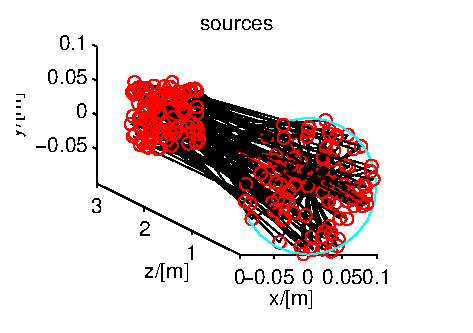
\includegraphics[width=0.9\textwidth]{figures/sources.eps}
  \end{center}
\caption{A source component that emits neutron events randomly, either from a model, or from a data file.}
\label{f:source}
\end{figure}

\newpage
\section{Source\_simple: A simple continuous source
with a flat energy/wavelength spectrum}
\label{source-simple}
\index{Sources!Source\_simple}

\component{Source\_simple}{System}{ $r_{\rm s}$, $z_{\rm foc}$, $w$, $h$, $E_0$, $\Delta E$, $\Psi$}{$\lambda_0$, $d\lambda$}{Validated, position is the center of disk}

This component is
a simple source with a energy distribution which is uniform
in the range $E_0 \pm dE$
(or wavelength distribution in the range $\lambda_0 \pm d\lambda$).
This component is not used for detailed time-of-flight simulations,
so we put $t=0$ for all neutron rays.

The initial neutron ray position is chosen randomly from within a
circle of radius $r_{\rm s}$ in the $z=0$ plane.
This geometry is a fair approximation
of a cylindrical cold/thermal source with the beam going out along
the cylinder axis.

The initial neutron ray direction is focused within
a solid angle, defined by a rectangular target of width
$w$, height $h$, parallel to
the $xy$ plane placed at $(0,0,z_{\rm foc})$.

The initial weight of the created neutron ray, $p_0$, is set to the
energy-integrated flux, $\Psi$, times the source area, $\pi r_{\rm s}^2$
times a solid-angle factor, which is basically the
solid angle of the focusing rectangle.
See also the discussion on focusing in the \MCS\ Manual \ref{s:focus}.

This component replaces Source\_flux\_lambda, Source\_flat, Source\_flat\_lambda, and
Source\_flux.


\newpage
\section{Source\_div: A continuous source with specified divergence}
\label{source-div}
\index{Sources!Source\_div}

\component{Source\_div}{System}{ $w$, $h$, $\delta_h$, $\delta_v$, $E_0$, $\Delta E$}{$\lambda_0$, $\Delta\lambda$, gauss}{Validated}

{\bf Source\_div} is a rectangular source, $w \times h$ (in m), which emits a
beam of a specified divergence around the direction of the $z$ axis.
The beam intensity is uniform over
the whole of the source, and the energy (or wavelength) distribution
of the beam is uniform over the specified energy range
$E_0 \pm \Delta E$ (in meV), or alternatively
the wavelength range $\lambda_0 \pm \delta\lambda$ (in \AA ).

The source divergencies are $\delta_h$ and $\delta_v$ (FWHM in degrees).
If the \verb+gauss+ flag is set to 0 (default), 
the divergence distribution is uniform, otherwise it is Gaussian.

This component may be used as a simple model of the
beam profile at the end of a guide or at the sample position.



\newpage
\section{Source\_Maxwell\_3: A continuous source
with a Maxwellian spectrum}
\label{source-maxwell}
\index{Sources!Source\_Maxwell\_3}

\component{Source\_Maxwell\_3}{System}{ $h$, $w$, $d_{\rm foc}$, $xw$, $yh$, $\lambda_{\rm low}$, $\lambda_{\rm high}$, $I_1$, $T_1$}{$I_2$, $T_2$, $I_3$, $T_3$}{Validated}

This component is a source with a Maxwellian energy/wavelength distribution
sampled in the range $\lambda_{\rm low}$ to $\lambda_{\rm high}$.
The initial neutron ray position is chosen randomly from within a
rectangle of area $h \times w$ in the $z=0$ plane.
The initial neutron ray direction is focused within
a solid angle, defined by a rectangular target of width
$xw$, height $yh$, parallel to
the $xy$ plane placed at $(0,0,d_{\rm foc})$.
The energy distribution used is a sum of 1, 2, or 3 Maxwellians with
temperatures $T_1$ to $T_3$ and integrated intensities $I_1$ to $I_3$.

The initial weight of the created neutron ray, $\pi_1$, is
calculated in the following way for one single Maxwellian:
The intensity in a small wavelength interval $[\lambda, \lambda+d\lambda]$ is
$ I_1 M(\lambda,T_1) d\lambda $
where
$M(\lambda,T_1) = 2 \alpha^2 \exp(-\alpha/\lambda^2) / \lambda^5 $ 
is the normalized Maxwell distribution ($\alpha=949.0$~K \AA$^2/T_1$).
The number of neutrons per second through a focusing window
of solid angle $\Omega$
from a source of area $A$ within the wavelength interval $\lambda_1$ to
$\lambda_2$ is thus
\begin{equation}
I_{\rm tot} = \Omega A \int_{\lambda_1}^{\lambda_2} I_1 M(\lambda,T_1) d\lambda.
\end{equation}
In a Monte Carlo integration, the observed intensity becomes
\begin{equation}
I_{\rm MC} \approx N_{\rm MC} \int p(\lambda) \pi_1(\lambda) d\lambda ,
\end{equation}
where $N_{\rm MC}$ is the number of Monte Carlo steps.
We here choose the wavelength from a uniform distribution between the two
limits, giving $p(\lambda)=1/(\lambda_2-\lambda_1)$.
To fulfill $I_{\rm tot} = I_{\rm MC}$ we need to have
\begin{equation}
\pi_1(\lambda) = \Omega A (\lambda_2-\lambda_1) I_1 M(\lambda,T_1) / N_{\rm MC} .
\end{equation}

%This expression is strictly valid only for $\Omega \ll 1$,
%see also the discussion on focusing in section \ref{s:focus}.
The expression is easily generalized to a general number of Maxwellians.

The component {\bf Source\_gen} (see section \ref{source-gen}) 
works on the same principle, but provides more options concerning 
wavelength/energy range specifications, shape, etc.



\newpage
\section{Source\_gen: A general continuous source}
\label{source-gen}
\index{Sources!General continuous source}

\component{Source\_gen}{(System) E. Farhi, ILL}{$w$, $h$, $xw$, $yh$, $E_0$, $\Delta E$, $T_1$, $T_2$, $T_3$, $I_1$, $I_2$, $I_3$ }{$r$, $\lambda_0$, $d\lambda$, $E_{min}$, $E_{max}$, $\lambda_{min}$, $\lambda_{max}$}{Validated for Maxwellian expressions. t=0}

This component is a continuous neutron source (rectangular or circular), which aims at
a rectangular target centered at the beam.
The angular divergence is given by the dimensions of the target.
The shape may be rectangular (dimension $h$ and $w$), or a disk of radius $r$.
The wavelength/energy range to emit is specified either using center and half width, or using minimum and maximum boundaries, alternatively for energy and wavelength.
The flux spectrum is specified with the same Maxwellian parameters as in component Source\_Maxwell\_3 (refer to section \ref{source-maxwell}).

Maxwellian parameters for some continuous sources
are given in Table~\ref{t:source_gen-params}. As nobody knows exactly the characteristics of the sources (it is not easy to measure spectrum there), these figures should be used with caution.

\begin{table}
  \begin{center}
  {\let\my=\\
    \begin{tabular}{|c|cccccc|c|}
    \hline
    Source Name & $T_1$ & $I_1$ & $T_2$ & $I_2$ & $T_3$ & $I_3$ & factor \\
    \hline
    PSI cold source & 150.4  & 3.67e11   & 38.74 & 3.64e11    & 14.84& 0.95e11   & * $I_{\rm target}$~(mA)\\
    ILL VCS (H1)    & 216.8  & 1.24e13   & 33.9  & 1.02e13    & 16.7 & 3.042e12  &\\
    ILL HCS (H5)    & 413.5  & 10.22e12  & 145.8 & 3.44e13    & 40.1 & 2.78e13   &\\
    ILL Thermal(H2) & 683.7  & 5.874e12  & 257.7 & 2.51e13    & 16.7 & 1.034e12  & /2.25\\
    ILL Hot source  & 1695   & 1.74e13   & 708   & 3.9e12     &      &           &\\ \hline
    \end{tabular}
    \caption{Flux parameters for present sources used in components
             Source\_gen and Source\_Maxwell\_3.
             For some cases, a correction factor to the intensity
             should be used to reach measured data; for the PSI cold source,
             this correction factor is the beam current, $I_{\rm target}$,
             which is currently of the order 1.2~mA.
}
    \label{t:source_gen-params}
  }
  \end{center}
\end{table}

\newpage
\section{Source\_adapt: A neutron source with adaptive importance sampling}
\label{s:Source_adapt}
\label{s:source-adapt}
\index{Optimization}
\index{Sources!Adaptive source}

\component{Source\_adapt}{K. Nielsen}{$x_{min}$, $x_{max}$, $y_{min}$, $y_{max}$, $E0$, $dE$, dist, $xw$, $yh$, $\Phi$}{$\alpha$, $\beta$ (plenty, default values are ok)}{partially validated}

{\bf Source\_adapt} is a neutron source that uses adaptive
importance sampling to improve the efficiency of the simulations. It
works by changing on-the-fly the probability distributions from which
the initial neutron state is sampled so that samples in regions that
contribute much to the accuracy of the overall result are preferred over
samples that contribute little. The method can achieve improvements of a
factor of ten or sometimes several hundred in simulations where only a
small part of the initial phase space contains useful neutrons.
This component uses the correlation between neutron energy,
initial direction and initial position.

The physical characteristics of the source are similar to those of
{\bf Source\_simple} (see section~\ref{source-simple}). The source is a thin
rectangle in the $x$-$y$ plane with a flat energy spectrum in a
user-specified range. The flux, $\Phi$, per area per steradian per
{\AA}ngstr{\o}m per second is specified by the user.

The initial neutron weight is given by Eq. (\ref{proprule}) using
$\Delta\lambda$ as the total wavelength range of the source.
A later version of this component will probably include a
$\lambda$-dependence of the flux.

We use the input parameters \textit{dist}, \textit{xw}, and \textit{yh}
to set the focusing as for Source\_simple (section~\ref{source-simple}).
The energy range will be from $E_0 - dE$ to $E_0 + dE$.
\textit{filename} is used to give the name of a file in which to
output the final sampling destribution, see below.
$N_{\rm eng}$, $N_{\rm pos}$, and $N_{\rm div}$
are used to set the number of bins in each dimensions.
Good general-purpose values for the optimization parameters are
$\alpha = \beta = 0.25$. The number of bins to choose will depend on the
application. More bins will allow better adaption of the sampling, but
will require more neutron histories to be simulated before a good
adaption is obtained. The output of the sampling distribution is only
meant for debugging, and the units on the axis are not necessarily
meaningful. Setting the filename to \verb+NULL+ disables the output of
the sampling distribution.

\subsection{Optimization disclaimer}

A warning is in place here regarding potentially wrong results
using optimization techniques.
It is highly recommanded in any case to benchmark 'optimized' simulations
against non-optimized ones, checking that obtained results are the same,
but hopefully with a much improved statistics.

\subsection{The adaption algorithm}

The adaptive importance sampling works by subdividing the initial
neutron phase space into a number of equal-sized bins. The division is
done on the three dimensions of energy, horizontal position, and
horizontal divergence, using $N_{\rm eng}$, $N_{\rm pos}$, and $N_{\rm
  div}$ number of bins in each dimension, respectively. The total number
of bins is therefore
\begin{equation}
N_{\rm bin} = N_{\rm eng} N_{\rm pos} N_{\rm div}
\end{equation}
Each bin $i$ is assigned a sampling weight $w_i$; the probability of
emitting a neutron within bin $i$ is
\begin{equation}
P(i) = \frac{w_i}{\sum_{j=1}^{N_{\rm bin}} w_j}
\end{equation}
In order to avoid false learning, the sampling weight of a bin is
kept larger than $w_{\rm min}$, defined as
\begin{equation}
w_{\rm min} = \frac{\beta}{N_{\rm bin}}\sum_{j=1}^{N_{\rm bin}}w_j,\qquad
    0 \leq \beta \leq 1
\end{equation}
This way a (small) fraction $\beta$ of the neutrons are sampled
uniformly from all bins, while the fraction $(1 - \beta)$ are sampled in an adaptive way.

Compared to a uniform sampling of the phase space (where the probability
of each bin is $1/N_{\rm bin}$), the neutron weight
must be adjusted as given by (\ref{probrule})
\begin{equation}
\pi_1 = \frac{P_1}{f_{\rm MC,1}} =\frac{1/N_{\rm bin}}{P(i)} =
    \frac{\sum_{j=1}^{N_{\rm bin}} w_j}{N_{\rm bin} w_i} ,
\end{equation}
where $P_1$ is understood by the "natural" uniform sampling.

In order to set the criteria for adaption, the {\bf Adapt\_check} component is
used (see section~\ref{s:adapt_check}). The source attemps to sample
only from bins from which neutrons are not absorbed prior to the
position in the instrument at which {\bf Adapt\_check} is
placed. Among those bins, the algorithm attemps to minimize the variance
of the neutron weights at the {\bf Adapt\_check} position. Thus bins that
would give high weights at the {\bf Adapt\_check} position are sampled more
often (lowering the weights), while those with low weights are sampled
less often.

Let $\pi = p_{\rm ac}/p_0$ denote the ratio between the neutron weight $p_1$ at
the {\bf Adapt\_check} position and the initial weight $p_0$ just after the
source. For each bin, the component keeps track of the sum $\Sigma$ of
$\pi$'s as well as of the total number of neutrons $n_i$ from that
bin. The average weight at the {\bf Adapt\_source} position of bin $i$ is thus
$\Sigma_i/n_i$.

We now distribute a total sampling weight of $\beta$ uniformly
among all the bins, and a total weight of $(1 - \beta)$ among bins in
proportion to their average weight $\Sigma_i/n_i$ at the {\bf Adapt\_source}
position:
\begin{equation}
w_i = \frac{\beta}{N_{\rm bin}} +
    (1-\beta) \frac{\Sigma_i/n_i}{\sum_{j=1}^{N_{\rm bins}} \Sigma_j/n_j}
\end{equation}
After each neutron event originating from bin $i$, the sampling weight $w_i$
is updated.

This basic idea can be improved with a small modification. The problem
is that until the source has had the time to learn the right sampling
weights, neutrons may be emitted with high neutron weights (but low
probability). These low probability neutrons may account for a large fraction of
the total intensity in detectors, causing large variances in the
result. To avoid this, the component emits early neutrons with a lower
weight, and later neutrons with a higher weight to compensate. This way
the neutrons that are emitted with the best adaption contribute the most
to the result.

The factor with which the neutron weights are adjusted is given by a
logistic curve
\begin{equation}
  F(j) = C\frac{y_0}{y_0 + (1 - y_0) e^{-r_0 j}}
\end{equation}
where $j$ is the index of the particular neutron history, $1 \leq j
\leq N_{\rm hist}$. The constants $y_0$, $r_0$, and $C$ are given by
\begin{eqnarray}
  y_0 &=& \frac{2}{N_{\rm bin}} \\
  r_0 &=& \frac{1}{\alpha}\frac{1}{N_{\rm hist}}
     \log\left(\frac{1 - y_0}{y_0}\right) \\
  C &=& 1 + \log\left(y_0 + \frac{1 - y_0}{N_{\rm hist}}
     e^{-r_0 N_{\rm hist}}\right)
\end{eqnarray}
The number $\alpha$ is given by the user and specifies (as a fraction
between zero and one) the point at which the adaption is considered
good. The initial fraction $\alpha$ of neutron histories are emitted
with low weight; the rest are emitted with high weight:
\begin{equation}
  p_0(j) =
    \frac{\Phi}{N_{\rm sim}} A \Omega \Delta\lambda
    \frac{\sum_{j=1}^{N_{\rm bin}} w_j}{N_{\rm bin} w_i}
    F(j)
\end{equation}
The choice of the constants $y_0$, $r_0$, and $C$ ensure that
\begin{equation}
\int_{t=0}^{N_{\rm hist}} F(j) = 1
\end{equation}
so that the total intensity over the whole simulation will be correct

Similarly, the adjustment of sampling weights is modified so that the
actual formula used is
\begin{equation}
w_i(j) = \frac{\beta}{N_{\rm bin}} +
    (1-\beta) \frac{y_0}{y_0 + (1 - y_0) e^{-r_0 j}}
     \frac{\psi_i/n_i}{\sum_{j=1}^{N_{\rm bins}} \psi_j/n_j}
\end{equation}

\subsection{The implementation}

The heart of the algorithm is a discrete distribution $p$. The
distribution has $N$ \emph{bins}, $1\ldots N$. Each bin has a value
$v_i$; the probability of bin $i$ is then $v_i/(\sum_{j=1}^N v_j)$.

Two basic operations are possible on the distribution. An \emph{update}
adds a number $a$ to a bin, setting $v_i^{\rm new} = v_i^{\rm old} +
a$. A \emph{search} finds, for given input $b$, the minimum $i$ such
that
\begin{equation}
 b \leq \sum_{j=1}^{i} v_j.
\end{equation}
The search operation is used to sample from the distribution p. If $r$
is a uniformly distributed random number on the interval
$[0;\sum_{j=1}^N v_j]$ then $i = {\rm search}(r)$ is a random number
distributed according to $p$. This is seen from the inequality
\begin{equation}
\sum_{j=1}^{i-1} v_j < r \leq \sum_{j=1}^{i} v_j,
\end{equation}
from which $r \in [\sum_{j=1}^{i-1} v_j; v_i + \sum_{j=1}^{i-1} v_j]$
which is an interval of length $v_i$. Hence the probability of $i$ is
$v_i/(\sum_{j=1}^N v_j)$.
The update operation is used to
adapt the distribution to the problem at hand during a simulation. Both
the update and the add operation can be performed very efficiently.

As an alternative, you may use the {\bf Source\_Optimizer} component
(see section \ref{source-optimizer}).


\newpage
% Emacs settings: -*-mode: latex; TeX-master: "manual.tex"; -*-

\section{Source\_Optimizer: A general Optimizer for McStas}
\label{s:sourceoptimizer}

This component was contributed by Emmanuel Farhi, Institute
Laue-Langevin.

The component {\bf Source\_Optimizer} optimizes the whole neutron flux
in order to achieve better statistics at each {\bf Monitor\_Optimizer}
location(s) (see section~\ref{s:monitoroptimizer} for this latter
component). It can act on any incoming neutron beam (from any source
type), and more than one optimization criteria location can be placed
along the instrument.

The usage of the optimizer is very simple, and usually does not require
any configuration parameter. Anyway the user can still customize the
optimization {\it via} various {\it options}.

The optimizer efficiency makes it easy to increase the number of events
at optimization criteria locations by a factor of 20, and thus decreases
the signal error bars by a factor 4.5. Higher factors can often be
achieved in practise. Of course, the overall flux remains the same as
without optimizer.

\subsection{The optimization algorithm}

When a neutron reaches the {\bf Monitor\_Optimizer} location(s), the
component records its position ($x$, $y$) and speed ($v_x,
v_y, v_z$) when it passed in the {\bf Source\_Optimizer}. Some
distribution tables of {\it good} neutrons characteristics are then
built.

When a {\it bad} neutron comes to the {\bf Source\_Optimizer} (it would
then have few chances to reach {\bf Monitor\_Optimizer}), it is changed
into a better one. That means that its position and velocity coordinates
are translated to better values according to the {\it good} neutrons
distribution tables. Anyway, the neutron energy ($\surd v_x^2 + v_y^2 +
v_z^2$) is kept as far as possible.

The {\bf Source\_Optimizer} works as follow:
\begin{enumerate}
\item{First of all, the {\bf Source\_Optimizer} determines some limits
    ({\it min} and {\it max}) for variables $x, y, v_x, v_y, v_z$.}
\item{Then the component records the non-optimized flux distributions in
    arrays with {\it bins} cells (default is 10 cells). This constitutes
    the {\it Reference } source.}
\item{\label {SourceOptimizer:step3}The {\bf Monitor\_Optimizer} records
    the {\it good} neutrons (that reach it) and communicate an {\it
      Optimized} source to the {\bf Source\_Optimizer}. However, '{\it
      keep}' percent of the original {\it Reference} source is sent
    unmodified (default is 10 \%). The {\it Optimized} source is thus:

    \begin{center}
      \begin{tabular}{rcl}
        {\it Optimized} & = & {\it keep} * {\it Reference} \\
        & + & (1 - {\it keep}) [Neutrons that will reach monitor].
      \end{tabular}
    \end{center}
    }
\item{The {\bf Source\_Optimizer} transforms the {\it bad} neutrons into
    {\it good} ones from the {\it Optimized} source. The resulting
    optimised flux is normalised to the non-optimized one:
    \begin{equation}
      p_{optimized} = p_{initial} \frac{\mbox{Reference}}{\mbox{Optimized}},
    \end{equation}
    and thus the overall flux at {\bf Monitor\_Optimizer} location is
    the same as without the optimizer. Usually, the process sends more
    {\it good} neutrons from the {\it Optimized} source than than in the
    {\it Reference} one.
    The energy (and velocity) spectra of neutron beam is also kept, as
    far as possible. For instance, an optimization of $v_z$ will induce
    a modification of $v_x$ or $v_y$ to try to keep $|\vec{v}|$
    constant.
    }
\item{When the {\it continuous} optimization option is activated (by
    default), the process loops to Step (\ref{SourceOptimizer:step3})
    every '{\it step}' percent of the simulation. This parameter is
    computed automatically (usually around 10 \%) in {\it auto} mode,
    but can also be set by user.}
\end{enumerate}

During steps (1) and (2), some non-optimized neutrons with original
weight $p_{initial}$ may lead to spikes on detector signals. This is
greatly improved by lowering the weight $p$ during these steps, with the
{\it smooth} option.
The component optimizes the neutron parameters on the basis of
independant variables. Howver, it usually does work fine when these
variables are correlated (which is often the case in the course of the
instrument simulation).
The memory requirements of the component are very low, as no big
$n$-dimensional array is needed.

\subsection{Using the Source\_Optimizer}

To use this component, just install the {\bf Source\_Optimizer} after a
source (but any location is possible in principle), and use the {\bf
  Monitor\_Optimizer} at a location where you want to have better
statistics.

\begin{verbatim}
    /* where to act on neutrons */
    COMPONENT optim_s = Source_Optimizer(options="") 
    ...
    /* where to have better statistics */
    COMPONENT optim_m = Monitor_Optimizer( 
    xmin = -0.05, xmax = 0.05, 
    ymin = -0.05, ymax = 0.05,
    optim_comp = optim_s) 
    ...
    /* using more than one Monitor_Optimizer is possible */
\end{verbatim}

The input parameter for {\bf Source\_Optimizer} is a single {\it
  options} string that can contain some specific optimizer configuration
settings in clear language. The formatting of the {\it options}
parameter is free, as long as it contains some specific keywords, that
can be sometimes followed by values.

The default configuration (equivalent to {\it options} = "") is
\begin{center}
\begin{tabular}{rcl}
  {\it options} & = & "{\it continuous} optimization,
  {\it auto} setting, {\it keep} = 10, {\it bins} = 10, \\
  & & {\it smooth} spikes, and do {\it not free} energy during optimization".
\end{tabular}
\end{center}
The keyword modifiers {\it no} or {\it not} revert the next option.
Other options not shown here are:
\begin{verbatim}
verbose         displays optimization process (debug purpose).
unactivate      to unactivate the Optimizer.
file=[name]     Filename where to save optimized source distributions
\end{verbatim}
The {\it file} option will save the source distributions at the end of
the optimization. If no name is given the component name will be used,
and a '.src' extension will be added. By default, no file is generated.
The file format is in a McStas 2D record style.


\newpage
% Emacs settings: -*-mode: latex; TeX-master: "manual.tex"; -*-

\section{Monitor\_Optimizer: Optimization locations for the\\
  Source\_Optimizer}
\label{monitor-optimizer}
\index{Sources!Optimization location|see{Sources/Optimizer}}\index{Optimization}
\component{Source\_Optimizer}{E. Farhi, ILL}{optim\_comp}{$x_{min}$, $x_{max}$, $y_{min}$,$y_{max}$}{partially validated}

The {\bf Monitor\_Optimizer} component works with the {\bf
  Source\_Optimizer} component. See section~\ref{source-optimizer}
for usage.

The input parameters for {\bf Monitor\_Optimizer} are the rectangular
shaped opening coordinates $x_{min}$, $x_{max}$, $y_{min}$,
$y_{max}$, and the name of the associated instance of
{\bf Source\_Optimizer} used in the instrument description file (one word,
without quotes).

As many Monitor\_Optimizer instances as required may be used in an instrument, 
for possibly more than one optimization location. 
Multiple instances may all have an effect on the total intensity.


\newpage
\section{Other sources components}
\label{sources-seealso}

There are other ways to define a source.

Pulsed source components are available for the SNS ({\bf contrib/SNS\_source}), ISIS ({\bf contrib/ISIS\_moderator}) and potential ESS ({\bf ESS\_moderator\_long} and {\bf  ESS\_moderator\_short}) facilities. Additionally, the {\bf Moderator} component implements a simple pulse model.

When no model exists (e.g. not a Maxwellian distribution), you may have access to measurement, estimated flux distributions, event files, and - better - to MCNP/Triploli4 neutron event records. The following components are then for you.

\begin{enumerate}
\item{{\bf misc/Virtual\_input} can read a \MCS\ event file (in text or binary format), often bringing a factor 10 speed-up. See section \ref{virtual_input}.}
\item{{\bf contrib/Virtual\_tripoli4\_input} does the same, but from event files (text format) obtained from the \emph{Tripoli4} \cite{tripoli_webpage} reactor simulation program. Such files are usually huge.}
\item{{\bf misc/Vitess\_input} can read \emph{Vitess} \cite{vitess_webpage} neutron event binary files.}
\item{{\bf optics/Filter\_gen} reads a 1D distributionb from a file, and may either modify or set the flux according to it.}
\item{A component for reading MCNP "PTRAC" records is planed for a next release. Contact us if you wish to participate.}
\end{enumerate}

% Emacs settings: -*-mode: latex; TeX-master: "manual.tex"; -*-

\chapter{Beam optical components:
Arms, slits, collimators, and filters}
This chapter contains a number of optical components
that is used to modify the neutron beam in various ways,
as well as the ``generic'' component {\bf Arm}.
\index{Library!Components!optics}
\index{Optics|textbf}

\section{Arm: The generic component}
\label{explain:arm}
\component{Arm}{System}{(none)}{(none)}{}
\index{Optics!Point in space (Arm, Optical bench)}

The component {\bf Arm} is empty; is resembles an optical bench
and has no effect on the xray.
The purpose of this component is only to provide a standard
means of defining a local coordinate system within the instrument definition.
Other components may then be
positioned relative to the {\bf Arm} component
using the \MCX\ meta-language.
The use of {\rm Arm} components in the instrument definitions
is not required but is recommended for clarity.
{\bf Arm} has no input parameters.

The first Arm instance in an instrument definition may be changed into a \verb+Progress_bar+(sec.~\ref{misc:Progress\bar}) component in order to display simulation progress on the fly , and possibly save intermediate results.


\section{Slit: A beam defining diaphragm}
\label{slit}

\component{Slit}{System}{$x_{\rm min}$, $x_{\rm max}$, $y_{\rm min}$, $y_{\rm max}$, $r$}{$p_{\rm cut}$}{}

The component {\bf Slit} is a very simple construction.
It sets up an opening at $z=0$, and propagates the neutrons
onto this plane (by the kernel call PROP\_Z0).
Neutrons within the slit opening are unaffected,
while all other neutrons
are discarded by the kernel call ABSORB.

By using this simple slit, some neutrons contributing to the background
in a real experiment will be neglected.
These are the ones that scatter off the inner side
of the slit, penetrates the slit material,
or clear the outer edges of the slit.

The input parameters of {\bf Slit} are the four coordinates,
$(x_{\rm min}, x_{\rm max}, y_{\rm min}, y_{\rm max})$
defining the opening of the rectangle, or the radius $r$ of
a circular opening, depending on which parameters are specified.

The slit component can also be used to discard unsignificant (very low weight)
neutron rays, that in some simulations may be very abundant and therefore
time consuming. If the optional parameter $p_{\rm cut}$ is set, all
neutron rays with $p<p_{\rm cut}$ are ABSORB'ed.




\section{Beamstop: A photon absorbing area}
\label{beamstop}
\index{Optics!Beam stop}

\component{Beamstop}{System}{$x_{min}$, $x_{max}$, $y_{min}$, $y_{max}$}{$r$}{}

The component {\bf Beamstop} can be seen as the reverse of
the {\bf Slit} component.
It sets up an area at the $z=0$ plane. Photons that hit the plane 
within this area are ABSORB'ed, while all others are unaffected.

By using this component, some photons contributing to the background
in a real experiment will be neglected.
These are the ones that scatter off the side
of the (real) beamstop, or penetrate the absorbing material.
Further, the holder of the beamstop is not simulated.

{\bf Beamstop} can be either circular or rectangular.
The input parameters of {\bf Beamstop} are either height and width $(x_{width},y_{height})$ or the four coordinates,
$(x_{\rm min}, x_{\rm max}, y_{\rm min}, y_{\rm max})$
defining the opening of a rectangle, or the radius $r$ of
a circle, depending on which parameters are specified.

If the "direct beam" (e.g. after a monochromator or sample) should not be
simulated, it is possible to emulate an ideal beamstop 
so that only the scattered beam is left;
without the use of {\bf Beamstop}:
This method is useful for instance in the case where only photons 
scattered from a sample are of interest. 
The example below removes the direct beam and 
any background signal from other parts of the instrument
\begin{verbatim}
COMPONENT MySample=V_sample(...) AT (...)
EXTEND
%{
  if (!SCATTERED) ABSORB;
%}
\end{verbatim}


\section{Filter\_gen: A general filter using a transmission table}
\label{filter-gen}
\index{Optics!Filter}
\index{Sources!from 1D table input}

\component{Filter\_gen}{System}{$x_{min}$, $x_{max}$, $y_{min}$, $y_{max}$, $file$}{$options$}{validated, flat filter}

This component is an ideal flat filter 
that changes the neutron flux according to a 1D input table (text file).

{\bf Filter\_gen} may act as a source ($options$="set") 
or a filter ($options$="multiply", default mode). 
The table itself is a 2 column free format file which accept comment lines. 
The first table column represent wavevector, energy, or wavelength, 
as specified in the $options$ parameter, 
whereas the second column is the transmission/weight modifier.

A usage example as a source would use 
\verb+options="wavelength, set"+, if the first column in the data 
is supposted to be $\lambda$ (in \AA ). 
Another example using the component as a filter would be 
\verb+options="energy, multiply"+ if the first column is $E$ (in meV).

The input parameters are the filter window size 
$x_{min}$, $x_{max}$, $y_{min}$, $y_{max}$, 
the behaviour specification string $options$ and the file to use $file$. 
Additionally, rescaling can be made automatic with the $scaling$ 
and relative $thickness$ parameters.

Some example data files are given with \MCS\ in the 
\verb+MCSTAS/data+ directory as \verb+*.trm+ files for transmission. 

A filter with finite thickness can be simulated by 
surrounding this component with two slits.

\newpage
\section{Collimator\_linear: The simple Soller blade collimator}

\component{Collimator\_linear}{System}{$x_{\rm min}$, $x_{\rm max}$, $y_{\rm min}$, $y_{\rm max}$,, $L$, $\delta$ (in deg.)}

The component {\bf Collimator\_linear} 
models a standard linear Soller blade collimator.
The collimator has two identical rectangular openings,
defined like the one in {\bf Slit}. Neutrons not clearing both
openings are ABSORB'ed, see the discussion in \ref{slit}.
The collimating effect is taken care of by employing an ideal
triangular transmission through the collimator, as explained below.
For a more detailed Soller collimator simulation,
taking every blade into accountm , the {\bf Channeled\_guide}
component can be employed, see section~\ref{s:channeled_guide}.

Let $L$ be the length of the collimator blades
and $d$ the distance between them.
Then let $\phi$ be the angle between the 
neutron path and the vertical $y-z$ plane along the collimator axis 
($\phi$ is also called the {\em horizontal divergence}).
We then define the collimation angle as the maximal allowed
horizontal divergence: $\delta = \tan^{-1}(d/L)$,
see Fig.~\ref{f:collimator}. Neutrons with a horizontal
divergence angle $|\phi| \geq \delta$ will always
hit at least one collimator blade and will thus be ABSORB'ed.
For smaller divergence angles, $|\phi| < \delta$, the fate of the
neutron depends on its exact entry point.
Assuming that a typical collimator has many blades, the
absolute position of each blade perpendicular to the collimator axis
is somewhat uncertain (and also unimportant in most cases).
A simple statistical consideration now shows that the transmission
probability is $T = 1-\tan|\phi|/\tan\delta$.

\begin{figure}
  \begin{center}
    \psfrag{xmin}[c][c]{$x_{\rm min}$}
    \psfrag{xmax}[c][c]{$x_{\rm max}$}
    \psfrag{ymin}[c][c]{$y_{\rm min}$}
    \psfrag{ymax}[c][c]{$y_{\rm max}$}
    \psfrag{delta}[c][c]{$\delta$}
    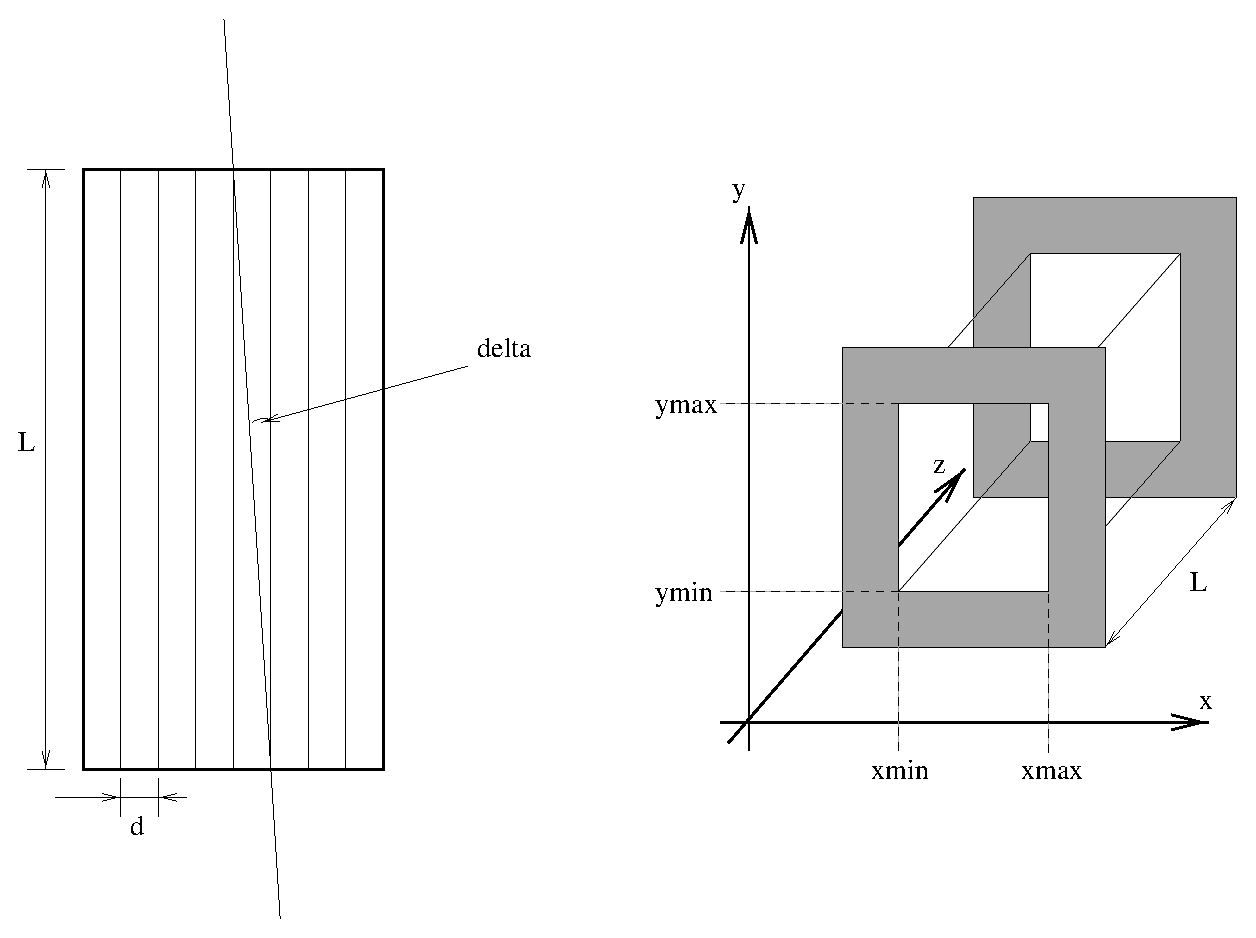
\includegraphics[width=0.9\textwidth]{figures/collimator.eps}
  \end{center}
\caption{The geometry of a simple Soller blade collimators:
The real Soller collimator, seen from the top (left), 
and a sketch of the component {\bf Soller} (right).
The symbols are defined in the text.}
\label{f:collimator}
\end{figure}

We simulate the collimator by transmitting all neutrons with
$|\phi| < \delta$, but adjusting their weight with the amount
\begin{equation}
\pi_i = T = 1-\tan|\phi|/ \tan\delta ,
\end{equation}
while all others are discarded by the kernel call ABSORB.
If $\delta=0$, the collimating effect is disabled,
so that $\pi_i = 1$ whenever the neutron clears the two apertures.


\section{Collimator\_radial: A radial Soller blade collimator}

\component{Collimator\_radial}{System, E.Farhi}{$w_1$, $h_1$, $w_2$, $h_2$, $len$, $\theta_{min}$, $\theta_{max}$, $nchan$, $radius$, $divergence$}{$nblades$, $roc$ and others}{validated, position is center of radius}

\begin{figure}
  \begin{center}
    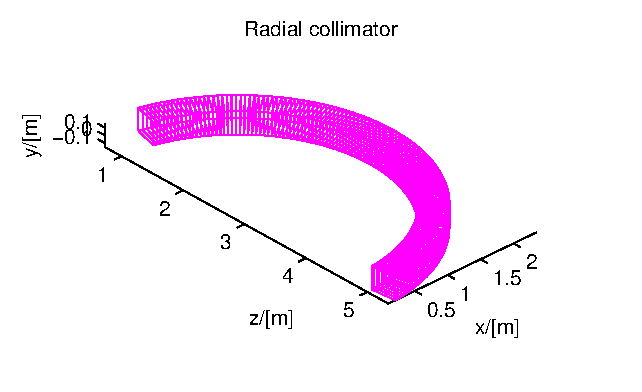
\includegraphics[width=0.9\textwidth]{figures/radial.eps}
  \end{center}
\caption{A radial collimator}
\label{f:coll-radial}
\end{figure}

This is a radial collimator that works either using the same approximation as the Collimator\_linear (see section \ref{collimator-linear}), or with an exact model but a lower statistics.

The geometry description requires to define the inner radius $radius$, the radial length $len$, the input and output window dimensions $w_1$, $h_1$, $w_2$, $h_2$, the number of Soller channels $nchan$ (each of then being a single linear collimator) arranged with the [$\theta_{min}$, $\theta_{max}$] angle with respect to the Z-axis.

If the $divergence$ parameter is defined, then the approximation level is used as in the Collimator\_linear component (see section \ref{collimator-linear}). On the other hand, if you perfer to describe exactly the number of blades $nblades$ assembled to build a single collimator channel, then the model is exact, and traces the neutron trajectory inside each Soller. The computing efficiency is then lowered by a factor 2.

The component can be made oscillating with an amplitude of $roc$ times $\pm w_1$.


\newpage
\chapter{Reflecting optical components: mirrors, and guides}
\index{Optics|textbf}

This section describes advanced neutron optical
components such as supermirrors and guides as well as various rotating choppers.
A description of the reflectivity of a supermirror is found
in section~\ref{s:mirror}.


\index{Optics|textbf}

This section describes advanced neutron optical
components such as supermirrors and guides.
A description of the reflectivity of a supermirror is found
in section~\ref{s:mirror}.

\section{Mirror: The single mirror}
\label{s:mirror}
\index{Optics!Mirror plane}
\component{Mirror}{System}{$l$, $h$, $m$}{$R_0, Q_c, W, \alpha$}{validated, no gravitation support}

The component {\bf Mirror}
models a single rectangular neutron mirror plate. It can be used
as a sample component or to \textit{e.g.}~assemble a complete neutron guide by putting multiple
mirror components at appropriate locations and orientations in the
instrument definition, much like a real guide is build from individual
mirrors.

In the local coordinate system, the mirror lies in the first quadrant of the
$x$-$y$ plane, with one corner at $(0,0,0)$.

The input parameters of this component are
the rectangular mirror dimensions $(l, h)$
and the values of $R_0, m, Q_c, W$, and $\alpha$ for the mirror reflectivity.
As a special case, if $m=0$ then the reflectivity is zero for all $Q$,
\textit{i.e.}\ the surface is completely absorbing.

This component may produce wrong results with gravitation.

\subsection{Mirror reflectivity}
\label{ss:mirrorreflect}
To compute the reflectivity of the supermirrors, we use an empirical
formula derived from experimental data \cite{pb_241_50},
see Fig.~\ref{f:reflectivity}. The reflectivity is given by
\begin{equation} \label{e:Rmirror}
  R = \left\{
    \begin{array}{ll}
      R_0 & \textrm{if $Q \leq Q_{\rm c}$} \\
      \frac{1}{2}R_0(1 - \tanh[(Q - m Q_{\rm c})/W])(1-\alpha(Q-Q_{\rm c}))
         & \textrm{if $Q > Q_{\rm c}$}
    \end{array}
  \right.
\end{equation}

Here $Q$ is the length of the scattering vector (in \AA$^{-1}$)
defined by
\begin{equation} \label{e:reflectivity}
Q = |{\bf k}_{\bf i} - {\bf k}_{\bf f}|
  = \frac{m_{\rm n}}{\hbar} |{\bf v}_{\bf i} - {\bf v}_{\bf f}|,
\end{equation}
$m_{\rm n}$ being the neutron mass.
The number $m$ in (\ref{e:Rmirror}) is a parameter determined by
the mirror materials,
the bilayer sequence, and the number of bilayers.
As can be seen, $R=R_0$ for $Q < Q_{\rm c}$, where $Q_{\rm c}$ is the
critical scattering wave vector for a single layer of the mirror
material. At higher values of $Q$, the reflectivity starts falling
linearly with a slope $\alpha$ until a "soft cut-off" at $Q = m Q_{\rm c}$.
The width of this cut-off is denoted $W$. See the example reflection curve in
figure~\ref{f:reflectivity}.

It is {\bf important} to notice that when $m < 1$, the reflectivity remains constant at $R=R_0$ up to $q=Qc$, and \emph{not} $m.Q_c$. This means that $m < 1$ parameters behave like $m=1$ materials.

\subsection{Algorithm}
The function of the component can be described as
\begin{enumerate}
\item Propagate the neutron ray to the plane of the mirror.
\item If the neutron trajectory intersects the mirror plate, it is
reflected, otherwise it is left untouched.
\item Reflection of the incident velocity
${\bf v}_{\rm i} = (v_x,v_y,v_z)$
gives the final velocity ${\bf v}_{\rm f} = (v_x,v_y,-v_z)$.
\item Calculate $Q=2 m_{\rm n} v_z / \hbar$.
\item The neutron weight is adjusted with the amount $\pi_i = R(Q)$.
\item  To avoid spending large amounts of computation time on very low-weight
neutrons, neutrons for which the reflectivity is lower than about
$10^{-10}$ are ABSORB'ed.
\end{enumerate}

\begin{figure}
  \begin{center}
    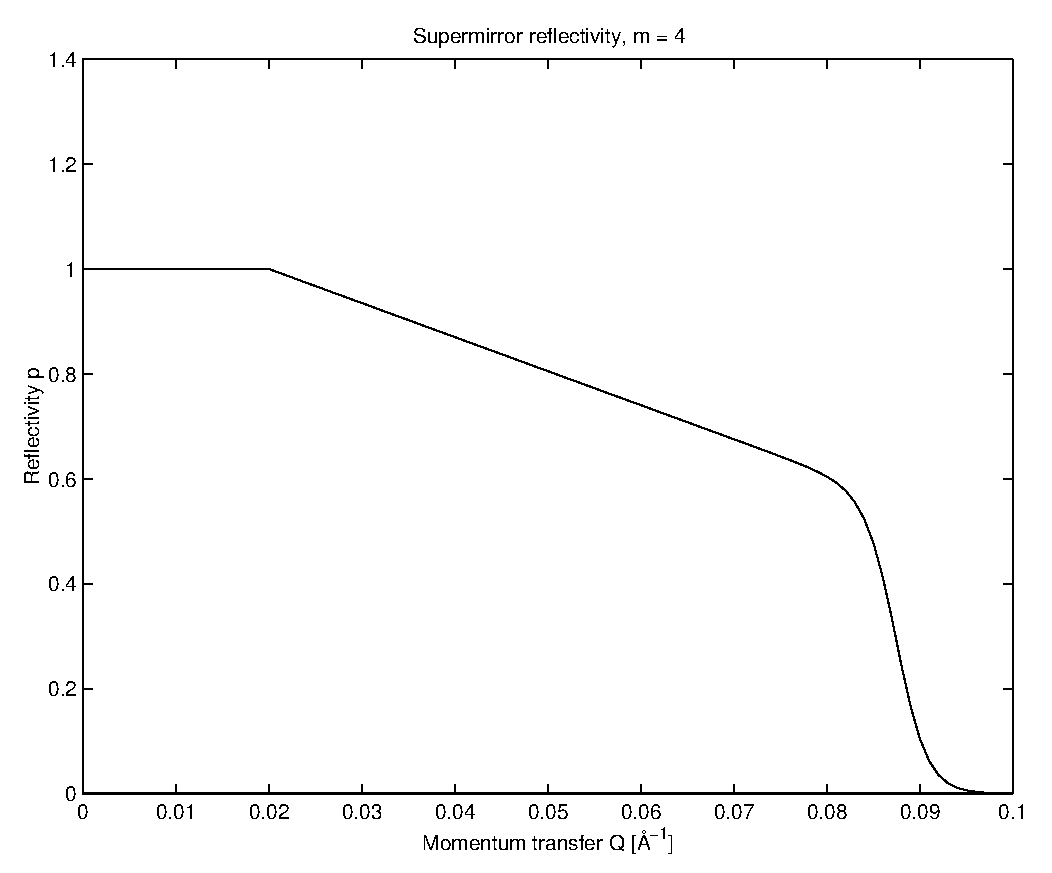
\includegraphics[width=0.6\textwidth]{figures/supermirror.eps}
  \end{center}
\caption{A typical reflectivity curve for a supermirror,
Eq.~(\protect\ref{e:reflectivity}). The used values are
$ m=4$, $R_0=1$, $Q_{\rm c} = 0.02$~\AA$^{-1}$, $\alpha = 6.49$~\AA,
$ W=1/300$~\AA$^{-1}$.
}
\label{f:reflectivity}
\end{figure}

\newpage

\section{Guide: The guide section}
\index{Optics!Straight guide}

\component{Guide}{System}{$w_1, h_1$, $w_2, h_2$, $l$, $m$}{$R_0, Q_c, W, \alpha$}{validated, no gravitation support}

The component {\bf Guide}
models a guide tube consisting of four flat mirrors. The
guide is centered on the $z$ axis with rectangular entrance and exit
openings parallel to the $x$-$y$ plane. The entrance has the dimensions
$(w_1,h_1)$ and placed at $z=0$. The exit is of dimensions $(w_2,h_2)$
and is placed at $z=l$ where $l$ is the guide length. See
figure~\ref{f:guide}.
The reflecting properties are given by the values of
$R_0, m, Q_c, W$, and $\alpha$, as for {\bf Mirror}.

{\bf Guide} may produce wrong results with gravitation support.
Use {\bf Guide\_gravity} (section \ref{s:guide_gravity}) in this case.
For a more general guide simulation, see {\bf Guide\_channeled}
in section~\ref{s:channeled_guide}.

\begin{figure}
  \begin{center}
    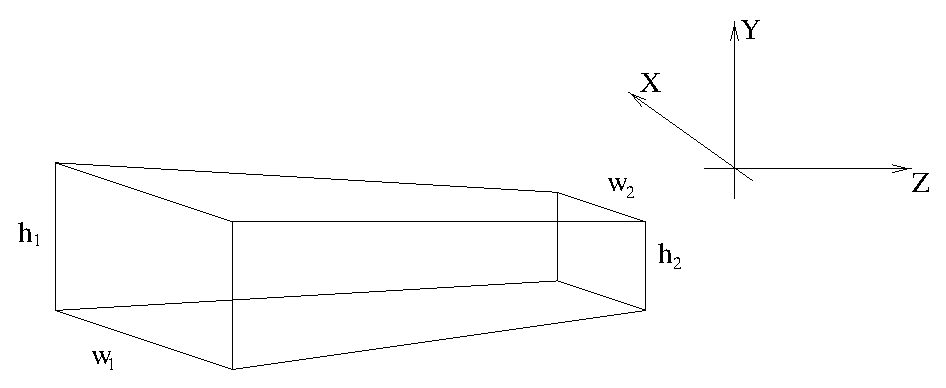
\includegraphics[width=0.7\textwidth]{figures/guide1.eps}
  \end{center}
\caption{The geometry used for the guide component.}
\label{f:guide}
\end{figure}

\subsection{Guide geometry and reflection}
For computations on the guide geometry, we define the planes of the four
guide sides by giving their normal vectors (pointing into the guide)
and a point lying in the plane:
$$
\begin{array}{rclcrcl}
{\bf n}^v_1 &=& (l, 0, {(w_2 - w_1) / 2})
     & & {\bf O}^v_1 &=& (- w_1 / 2, 0, 0) \\
{\bf n}^v_2 &=& (-l, 0, {(w_2 - w_1) / 2})
     & & {\bf O}^v_2 &=& (w_1 / 2, 0, 0) \\
{\bf n}^h_1 &=& (0, l, {(h_2 - h_1) / 2})
     & & {\bf O}^h_1 &=& (0, - h_1 / 2, 0) \\
{\bf n}^h_2 &=& (0, -l, {(h_2 - h_1) / 2})
     & & {\bf O}^h_2 &=& (0, h_1 / 2, 0) \\
\end{array}
$$
In the following, we refer to an arbitrary guide side by its origin
{\bf O} and normal {\bf n}.

With these definitions, the time of intersection of the neutron with a
guide side can be computed by considering the projection onto the
normal:
\begin{equation}
t^\alpha_\beta = \frac{({\bf O}^\alpha_\beta - {\bf r}_0) \cdot {\bf n}^\alpha_\beta}
  {{\bf v} \cdot {\bf n}^\alpha_\beta}  ,
\end{equation}
where $\alpha$ and $\beta$ are indices for the different guide walls,
assuming the values (h,v) and (1,2), respectively.
For a neutron that leaves the guide directly through the guide exit we have
\begin{equation}
t_{\rm exit} = \frac{l - z_0}{v_z}
\end{equation}

The reflected velocity ${\bf v}_{\rm f}$ of the neutron with incoming velocity
${\bf v}_{\rm i}$ is computed by the formula
\begin{equation}
 {\bf v}_{\rm f} =
  {\bf v}_{\rm i}
   - 2{{\bf n} \cdot {\bf v}_{\rm i} \over {|{\bf n}|^2}} {\bf n}
\end{equation}
This expression is arrived at by again considering the projection onto
the mirror normal (see figure~\ref{f:guidereflect}). The reflectivity of the
mirror is taken into account as explained in section~\ref{s:mirror}.

\begin{figure}
  \begin{center}
    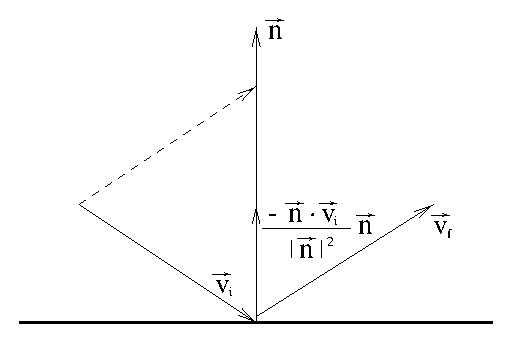
\includegraphics[width=0.5\textwidth]{figures/guide2.eps}
  \end{center}
\caption{Neutron reflecting from mirror. ${\bf v}_{\rm i}$ and
${\bf v}_{\rm f}$ are the initial and final velocities, respectively,
and {\bf n} is a vector normal to the mirror surface.}
\label{f:guidereflect}
\end{figure}

\subsection{Algorithm}
\begin{enumerate}
\item The neutron is initially propagated to the $z = 0$ plane of the
guide entrance.
\item If it misses the entrance, it is ABSORB'ed.
\item Otherwise, repeatedly compute the time of intersection with the
four mirror sides and the guide exit.
\item The smallest positive $t$ thus
found gives the time of the next intersection with the guide (or in the
case of the guide exit, the time when the neutron leaves the guide).
\item Propagated the neutron ray to this point.
\item Compute the reflection from the side.
\item Update the neutron weight factor by the amount $\pi_i = R(Q)$.
\item Repeat this process until the neutron leaves the guide.
\end{enumerate}

There are a few optimizations possible here to avoid redundant
computations. Since the neutron is always inside the guide during the
computations, we always have
$({\bf O} - {\bf r}_0) \cdot {\bf n} \leq 0$.
Thus $t \leq 0$ if ${\bf v} \cdot {\bf n} \geq 0$, so in this case
there is no need to actually compute $t$. Some redundant computations
are also avoided by utilizing symmetry and the fact that many
components of {\bf n} and {\bf O} are zero.

\newpage

\section{Guide\_channeled: A guide section component with multiple channels}
\label{s:channeled_guide}
\index{Optics!Guide with channels (straight, non focusing)}

\component{Guide\_channeled}{System}{$w_1, h_1$, $w_2, h_2$, $l$, $k$, $m_x, m_y$}{$d, R_0, Q_{cx}, Q_{cy}, W, \alpha_x, \alpha_y$}{validated, no gravitation support}

The component {\bf Guide\_channeled} is a more complex variation of {\bf Guide}
described in the previous section. It allows the specification
of different supermirror parameters for the horizontal and vertical
mirrors, and also implements guides with multiple channels as used in
neutron bender devices. By setting the $m$ value of the supermirror
coatings to zero, nonreflecting walls are simulated;
this may be used for a very detailed simulation of a Soller collimator,
see section~\ref{collimator-linear}.

The input parameters are $w_1$, $h_1$, $w_2$, $h_2$, and $l$
to set the guide dimensions as for {\bf Guide}
(entry window, exit window, and length);
$k$ to set the number of channels; $d$ to set the thickness of the
channel walls; and $R_0$, $W$, $Q_{cx}$, $Q_{cy}$, $\alpha_x$, $\alpha_y$,
$m_x$, and $m_y$ to set the supermirror parameters as described under {\bf Guide}
(the names with \textit{x} denote the vertical mirrors,
and those with \textit{y} denote the horizontal ones).

\subsection{Algorithm}
The implementation is based on that of {\bf Guide}.
\begin{enumerate}
\item Calculate the channel which the neutron will enter.
\item Shift the $x$ coordinate so that the channel can be simulated
as a single instance of the {\bf Guide} component.
\item (do the same as in {\bf Guide}.)
\item Restore the coordinates when the
neutron exits the guide or is absorbed.
\end{enumerate}

\subsection{Known problems}\index{Bugs}
\begin{itemize}
\item This component may produce wrong results with gravitation support.
Use Guide\_gravity (section \ref{s:guide_gravity}) in this case.
\item The focusing channeled geometry (for $k > 1$ and different
values of $w_1$ and $w_2$) is buggy
(wall slopes are not computed correctly, and the component 'leaks' neutrons).
\end{itemize}
\newpage

\section{Guide\_gravity: A guide with multiple channels and gravitation handling}
\label{s:guide_gravity}
\index{Optics!Guide with channels and gravitation handling (straight)}
\index{Optics!Fermi Chopper}

\component{Guide\_gravity}{System}{$w_1, h_1$, $w_2, h_2$, $l$, $k$, $m$}{$d, R_0, Q_c, W, \alpha$, wavy, chamfers, $k_h$, $n$, $G$}{validated, {\bf with} gravitation support, rotating mode}

This component is a variation of {\bf Guide\_channeled}
(section \ref{s:channeled_guide}) with the ability to handle
gravitation effects and functional channeled focusing geometry.
Channels can be specified in two dimensions,
producing a 2D array ($k, k_h$) on smaller guide channels.

Waviness effects, supposed to be randomly distributed
(\emph{i.e.} non-periodic waviness)
can be specified globally, or for each part of the guide section.
Additionally, chamfers
may be defined the same way.
Chamfers originate from the substrate manufacturing, so that operators do not harm themselves with cutting edges. Usual dimensions are about tens of millimeters. They are treated as absorbing edges around guide plates, both on the input and output surfaces, but also aside each mirror.

The straight section of length $l$ may be divided into $n$ bits of same length
within which chamfers are taken into account.

The component has also the capability to rotate at a given frequenccy in order to approximate a Fermi Chopper, including phase shift. The approximation resides in the fact that the component is considered fixed during neutron propagation inside slits.

To activate gravitation support, either select the \MCS\ gravitation support,
or set the gravitation field strength $G$ (e.g. -9.81 on Earth).

This component is about 50 \% slower than the \verb+Guide+ component, but has much more capabilities.

\section{Bender: a bender model (non polarizing)}
\index{Optics!Bender (non polarizing)}

\component{Bender}{Philipp Bernhardt}{$r, W_{in},l,w,h $}{$k,d,R_{0[a,i,s]},\alpha_{[a,i,s]},m_{[a,i,s]},Q_{c[a,i,s]},W_{[a,i,s]}$}{partly validated, no gravitation support}

The Bender component is simulating an ideal curved neutron guide (bender). It is bent to the negative X-axis and behaves like a parallel guide in the Y axis. Opposite curvature may be achieved by a $(0,0,180)$ rotation (along Z-axis).

Bender radius $r$, entrance width $w$ and height $h$ are required parameters. To define the length, you may either enter the deviation angle $W_{in}$ or the length $l$. Three different reflectivity profiles $R_0,Q_c,W,m,\alpha$ can be given (see section~\ref{s:mirror}): for outer
walls (index $a$), for inner walls (index $i$) and for the top and bottom walls (index $s$).

To get a better transmission coefficient, it is possible to split the bender into $k$ channels which are separated by partitions with the thickness of $d$. The partitioning walls have the same coating as the exterior walls.

Because the angle of reflection doesn't change, the routine
calculates the reflection coefficent for the concave and, if necessary, for the convex wall only onces, together with the number of reflections.
Nevertheless the exact position, the time, and the divergence is calculated at the end of the bender, so there aren't any approximations.

The component is shown \emph{straight} on geometrical views (mcdisplay/Trace), and the next component may be placed directly at distance $r.W_{in} = l$ \emph{without} rotation.

Results have been compared succesfully with analytical formula in the case of an ideal reflection and cross-checked with the program \verb+haupt+.

An other implementation of the Bender is available as the contributed component Guide\_curved.

\section{Curved guides}
\index{Optics!Curved guides (polygonal model)}

Real curved guides are usually made of many straight elements (about 1 m long) separated with small gaps (e.g. 1 mm). Sections of about 10 m long are separated with bigger gaps for accessibility and pumping purposes.

We give here an example description of such a section. Let us have a curved guide of total length $L$, made of $n$ elements with a curvature radius $R$. Gaps of size $d$ separate elements from each other. The rotation angle of individual straight guide elements is $\alpha_z = (L+d)/R*180/\pi$ in degrees.

In order to build an independent curved guide section, we define \verb+Arm+ components at the begining and end of it.
\begin{verbatim}
COMPONENT CG_In = Arm() AT (...)

COMPONENT CG_1  = Guide_gravity(l=L/n, ...)
AT (0,0,0) RELATIVE PREVIOUS

COMPONENT CG_2  = Guide_gravity(l=L/n, ...)
AT (0,0,L/n+d) RELATIVE PREVIOUS
ROTATED (0, (L/n+d)/R*180/PI, 0) RELATIVE PREVIOUS
...
COMPONENT CG_Out = Arm() AT (0,0,L/n) RELATIVE PREVIOUS
\end{verbatim}
The \verb+Guide+ component should be duplicated $n$ times by copy-paste, but changing the instance name, e.g. CG\_1, CG\_2, ..., CG\_n. This may be automated with the \verb+COPY+ or the \verb+JUMP ITERATE+ mechanisms (see User manual).

An implementation of a continuous curved guide has been contributed as component Guide\_curved.



\chapter{Moving optical components:
Choppers and velocity selectors}
We list in this chapter some moving optical components,
like chopper, that may be used for TOF class instrument simulations,
and velocity selector used for partially monochromatize continuous beams.
\index{Library!Components!optics}
\index{Optics|textbf}

% Emacs settings: -*-mode: latex; TeX-master: "manual.tex"; -*-

\section{Chopper: The disc chopper}
\label{s:chopper}

\component{Chopper}{Phillipp Bernhardt}{$w$, $R$, $f$, $n$, $\phi$}{IsFirst, $n_{\rm pulse}$}

To cut a continuous neutron beam into short pulses, or to control
the pulse shape from a pulsed source, one can use a disc
chopper (see figure~\ref{f:chopper1}). This is a fast rotating disc with the
rotating axis parallel to the neutron beam. The disk consists of neutron
absorbing materials. To form the pulses the disk has openings through which
the neutrons can pass.

\begin{figure}[ht]
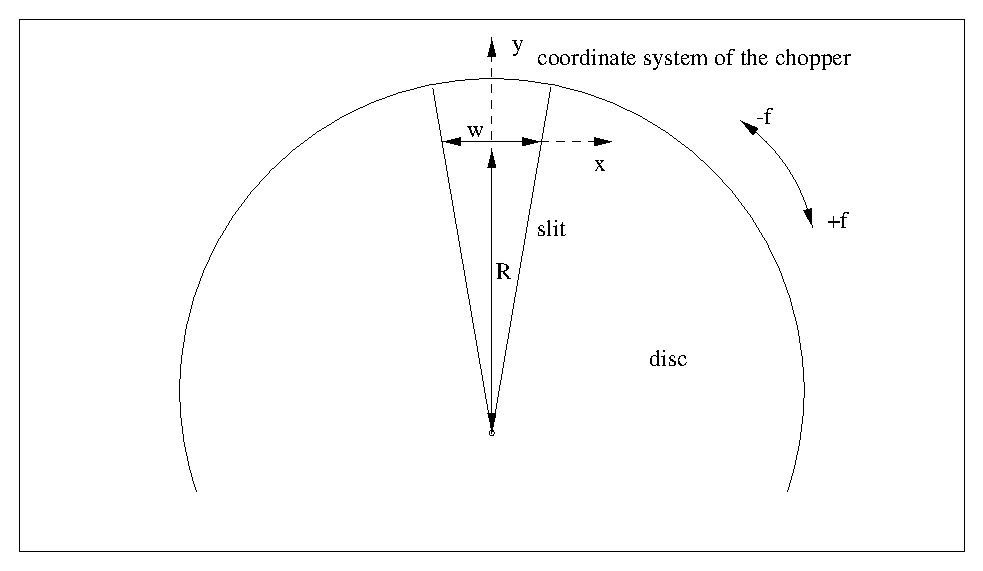
\includegraphics[width=1.0\linewidth]{figures/Chopper.eps}
\caption{disc chopper\label{f:chopper1}}
\end{figure}

Component {\bf Chopper} has $n$ openings, which are
symmetrically positioned on the disc. You can set the direction of
rotation, which allows to simulate double choppers. You can also define
the phase by setting the time at which one slit is positioned at the
top. The sides of the slits are pointing towards the center of the disc.
The thickness of the disc is neglected.  There is no parameter for the
size of the slits in the radial direction; 
use e.g. a {\bf Slit} component in front of the chopper.

Using a rectangular shaped beam with nearly the same
size as the slit, yields an almost triangular shaped
transmission curve (see figure~\ref{f:chopper2}).

\begin{figure}[ht]
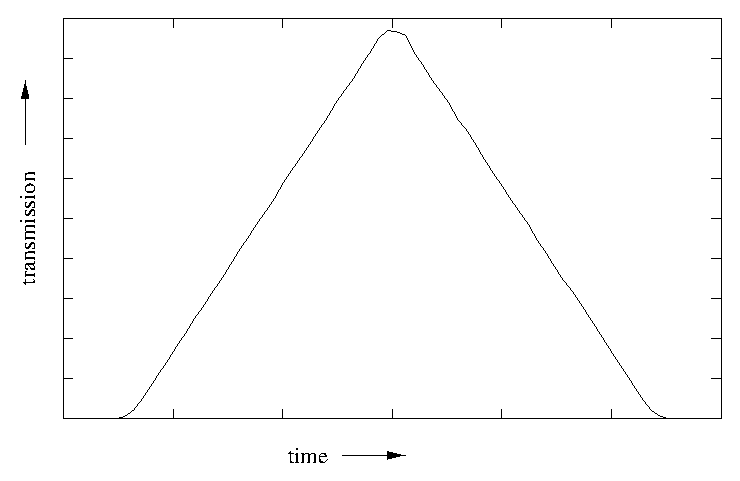
\includegraphics[width=1.0\linewidth]{figures/tracho.eps}
\caption{example transmission curve for the disc chopper\label{f:chopper2}}
\end{figure}    

When simulating the chopping of a continuous beam,
most of the neutrons could easily be lost.
To improve efficiency, one can set the flag \verb+IsFirst+, which will
allow every neutron ray to pass the {\bf Chopper}, but modify the 
time, $t$, to a time at which it is possible to pass. 
This can also be used with TOF-instruments, which often
define the starting time of the neutrons at
the position of the first chopper.
Of course, there should be only one ``first chopper'' in
any simulation.
To simulate frame overlap from a ``first chopper'', one can specify 
the number of frames to study by the parameter $n_{\rm pulse}$.

\newpage
\section{FermiChopper:The Fermi-chopper}

\component{FermiChopper}{M. Poehlmann, C. Carbogno, H. Schober, E. Farhi}{$R,y_{min} y_{max}, \nu,w,length$,Nslit,phase}{$m,Q_c,R_0,\alpha, W$,zero\_time}{validated}
\index{Optics!Fermi Chopper}

\begin{figure}
\begin{center}
\begin{tabular}{cc}
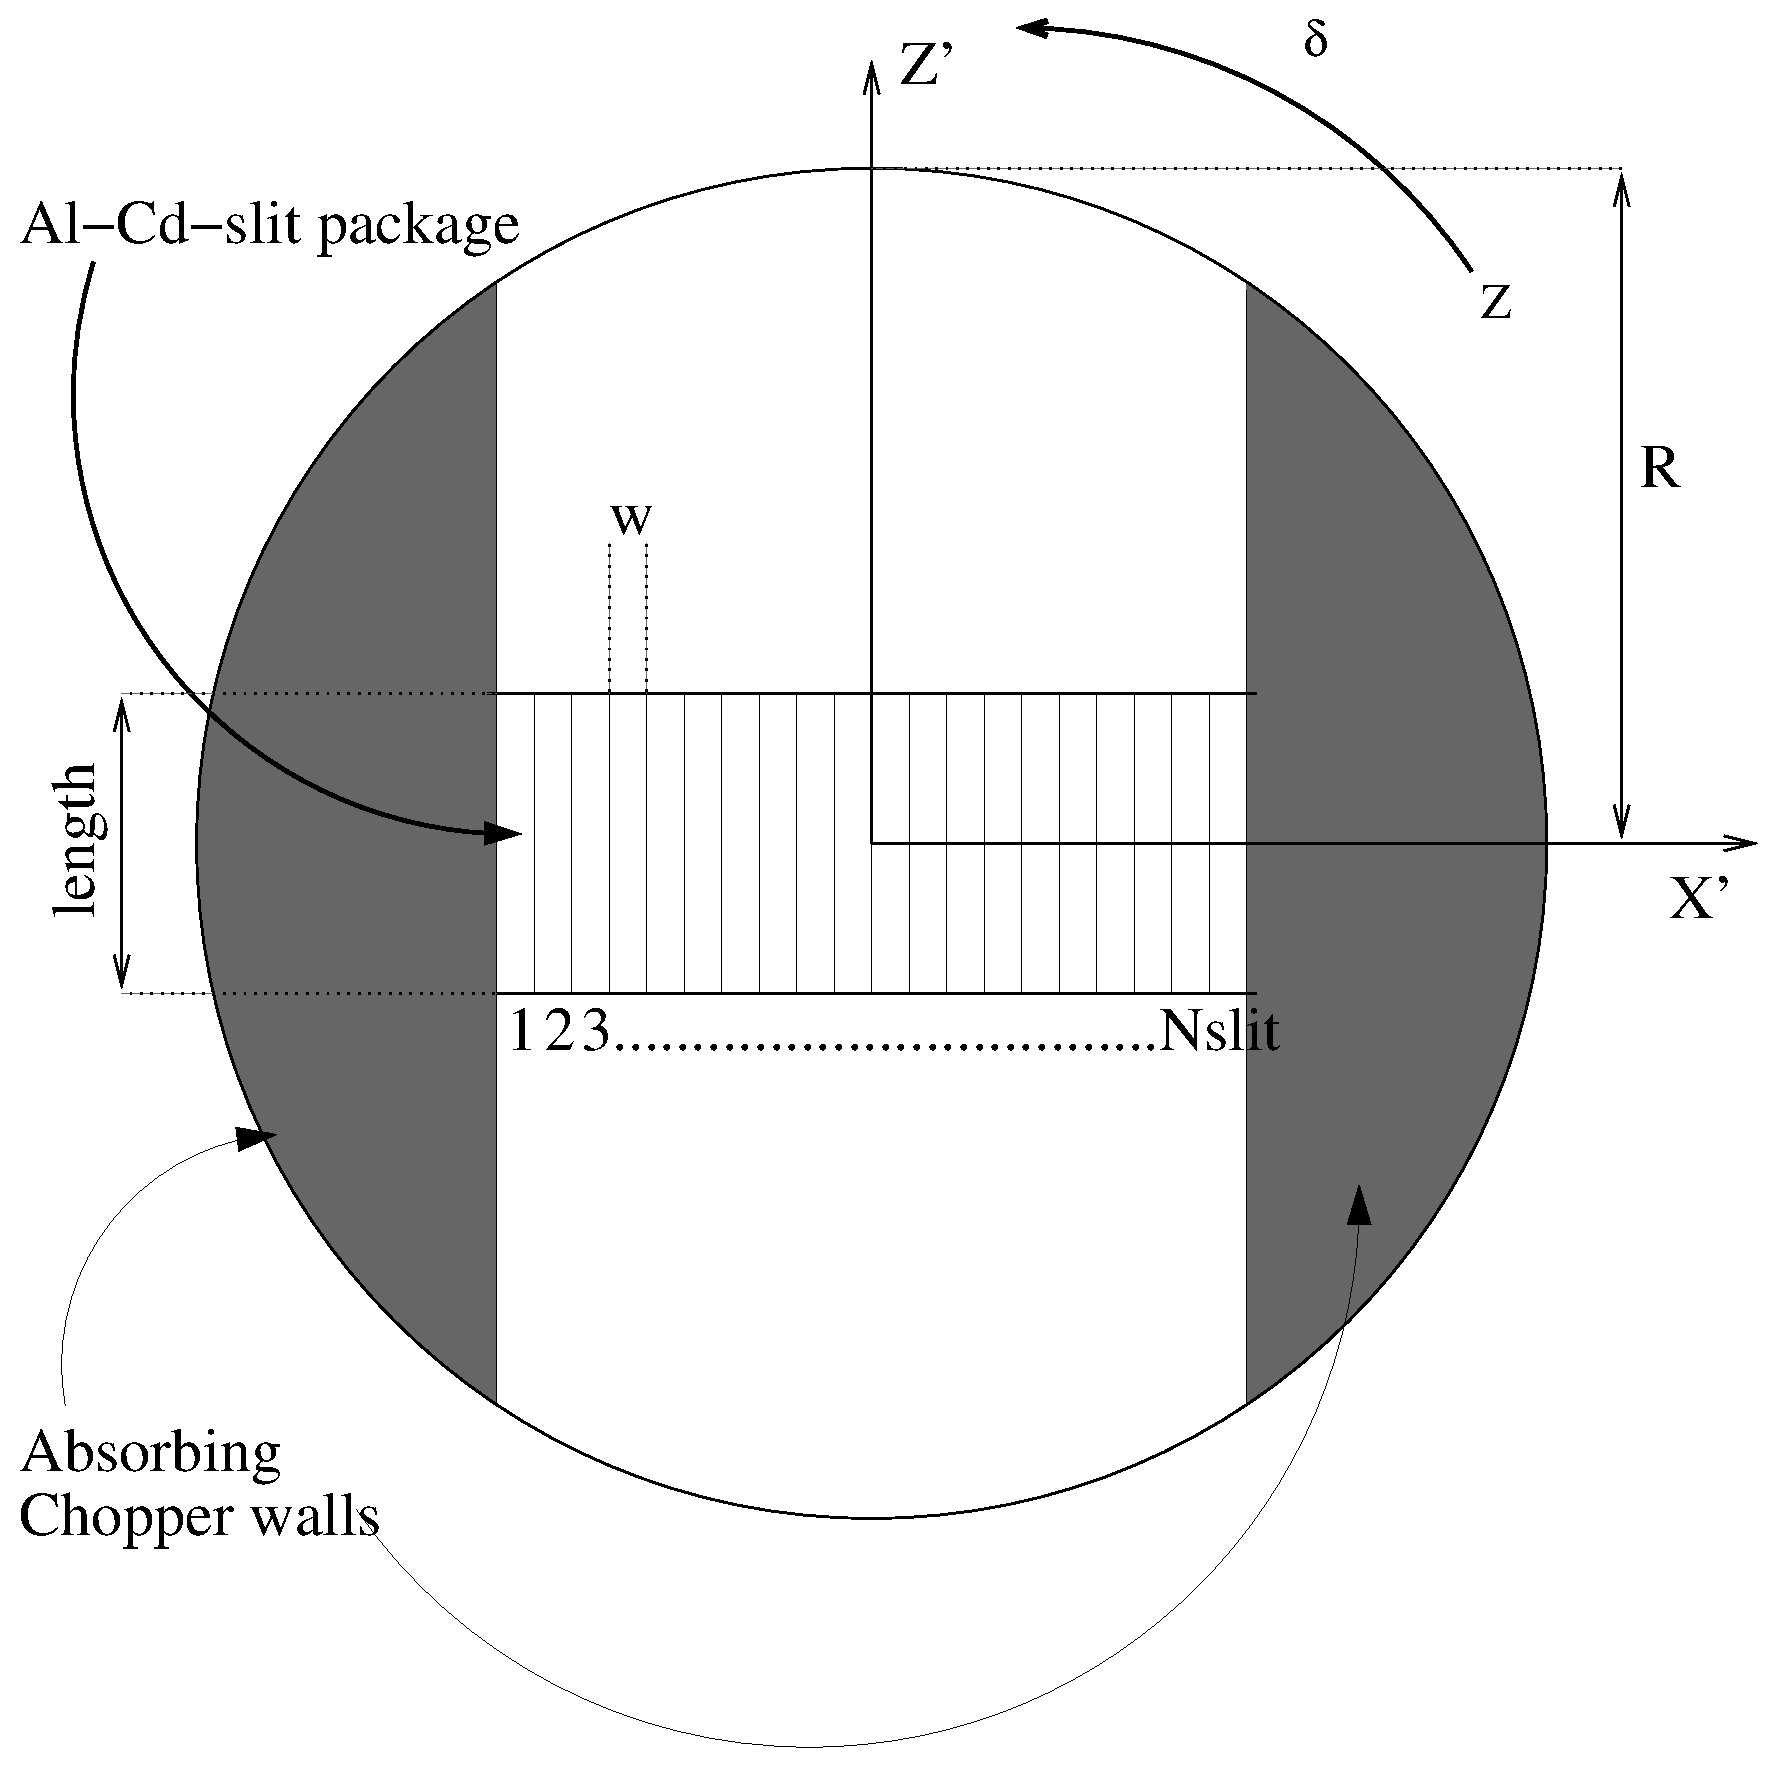
\includegraphics[height=7cm]{./figures/FCChoppergeo.eps}
&
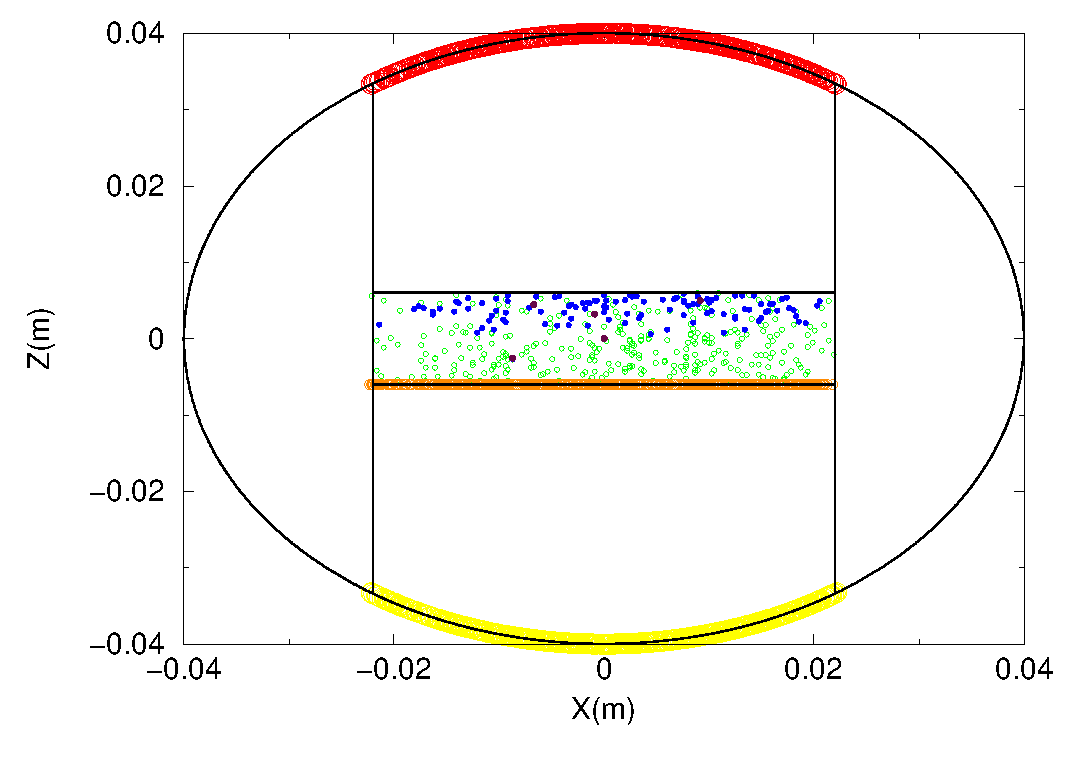
\includegraphics[height=5cm,width=5.3cm]{./figures/FCOverview.eps}
\end{tabular}
\end{center}
\caption{Geometry of the Fermi-chopper (left) and Neutrons in the chopper (right).}
\label{fig:Overview.eps}
\end{figure}

\subsection{The chopper geometry and parameters}
\label{ssec:chopper}

The Fermi chopper is a rotating vertical cylinder containing a set of collimating slits (\emph{slit package}). Main geometry parameters are the radius $R$, minimum and maximum height $y_{min}$ and $y_{max}$ (see Fig. \ref{fig:Overview.eps}).
In this implementation, the slits are straight, but may be coated with super-mirror. Main parameters for the slits are the number of slits $Nslit$, the length $length$ and width $w$ of each slit, the width of the separating Cd-blades is neglected. The slit walls reflectivity is modelled just like in guide components by the $m$-value ($m > 1$ for super mirrors), the critical scattering vector $Q_c$, the slope of reflectivity $\alpha$, the low-angle reflectivity $R_0$ and the width of supermirror cut-off $W$. For $m=0$ the blades are completly absorbing. The AT position of the component is its center.

The angular speed of the chopper is $\omega = 2\pi \nu$, where $\nu$ is the rotation frequency. The angle $phase$ for which the chopper is in the 'open' state for most of the neutrons coming in (z' axis of the rotating frame parallel to the z axis of the static frame) is also an input parameter. The time window may optionally be shifted to zero when setting the \verb+zero_time=1+ option.

The curvature of the slit channels is specified with the $R_{slit}$ parameter. Positive sign indicates that the deviation 'bump' due to curvature is in the positive side, and the center of curvature is in the $x'$ negative side.

The component was validated extensivelly by K. Lieutenant. As an alternative, and for curved slit packages, one may use the {\bf Vitess\_ChopperFermi} component.

\subsection{Propagation in the Fermi-chopper}

As can be seen in figure \ref{fig:Overview.eps}, neutrons first propagate onto the cylinder surface of the chopper (yellow curve). Then the program checks the interaction with the entrance of the slit package (orange line) and calculates which slit is hit. If the slit coating is reflecting ($m > 0$), multiple reflections are calculated (green, blue and maroon circles), otherwise the neutrons are absorbed as soon as they interact with the blades. Finally the remaining neutrons propagate to the exit of the chopper (red curve).

The rotation of the chopper is characterized by the angle $\delta$ between the rotating z' and the static z-axis. $\delta(t)$ is defined by:

$$\delta(t) = \widehat{z,z'} = \omega.(t-t_0)$$

where $t$ is the absolute time. The chopper should better be \emph{time focussing}: slow neutrons should pass before the fast ones, so that they finally hit the detectors at the same time. Therefore the signs of $\omega$ and $\delta$ are very important: For $t>t_0$, $\delta$ is positive and points anti-clockwise.

Since the rotation is applied along the y - axis, we can simplify the problem to two dimensions. The orthogonal transformation matrix $T$ from the static $(xz)$ to the rotating frame $(x'z')$ is:
\begin{equation}
T_{xz \rightarrow x'z'} = \left(
\begin{array}{cc}
\cos(\delta) & \sin (\delta) \\
-\sin(\delta) & \cos(\delta)
\end{array}
\right)
\end{equation}

\begin{figure}
\begin{center}
\begin{tabular}{cc}
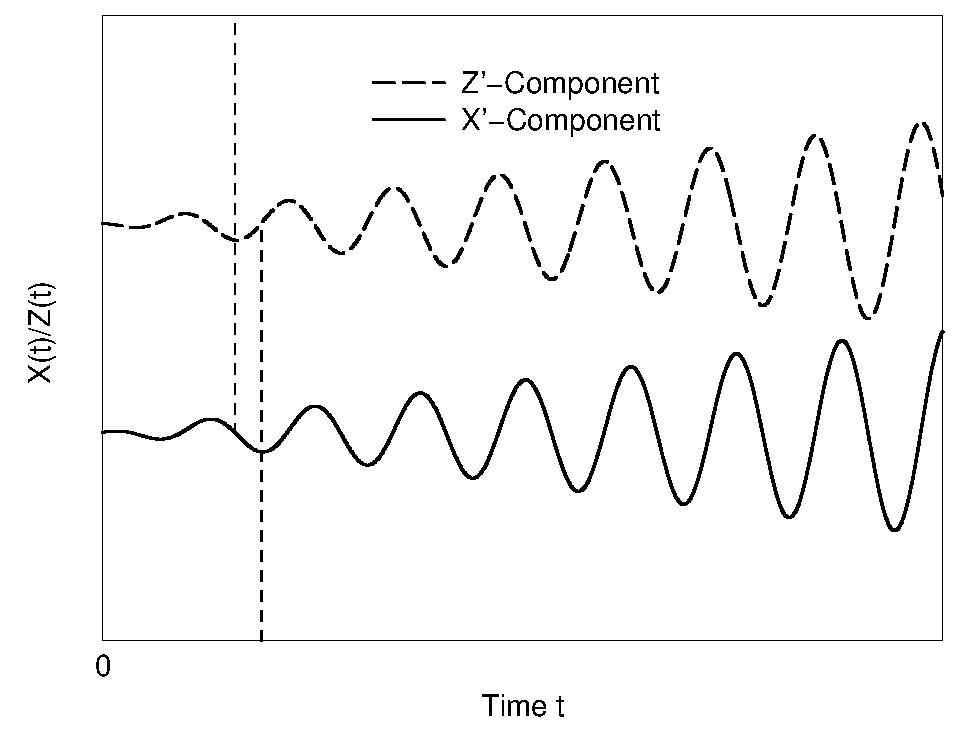
\includegraphics[height=5.5cm]{./figures/XZCoords.eps}
&
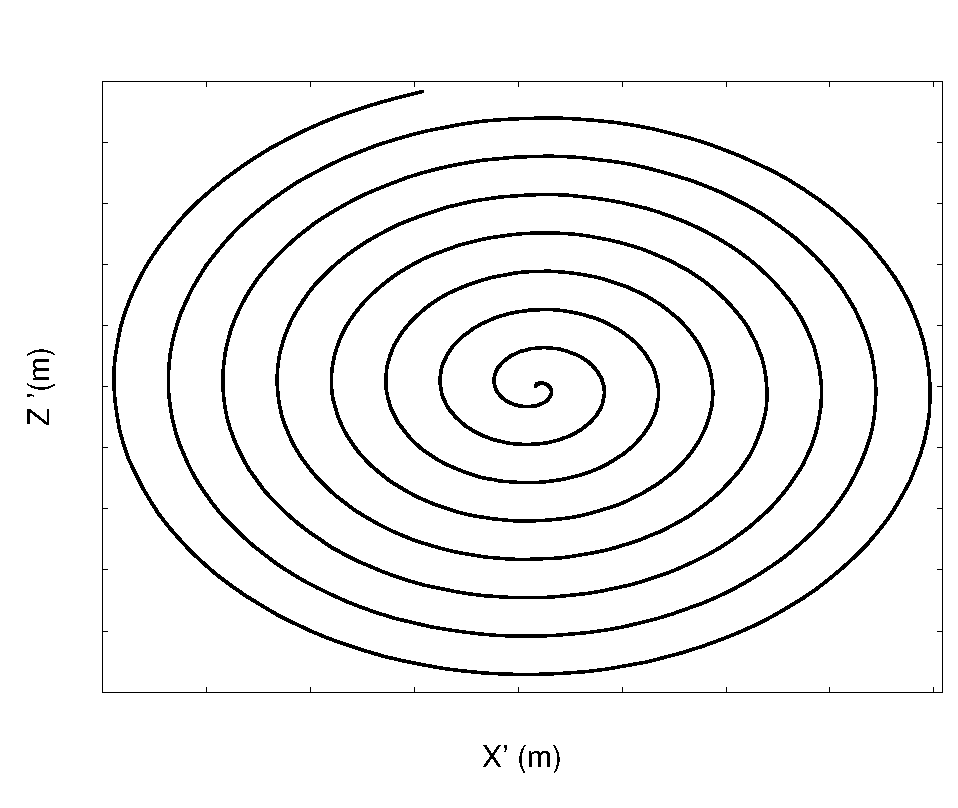
\includegraphics[height=6.5cm,width=5.5cm]{./figures/XZplain.eps}
\end{tabular}
\end{center}
\caption{The x' and z' component as a function of time in the rotating frame (left). A typical neutron trajectory in the rotating frame (right).}
\label{fig:Component.eps}
\end{figure}

Together with the equation for a non-accelerated, linear propagation $\vec{r} = \vec{r_0}+\vec{v}t$ the orthogonal transformation produces a curve in the X'-Z'-plane known as \emph{archidemic spiral}, as can be seen in figure \ref{fig:Component.eps}. The two vector components $s(t) = (x',z')$ follow the equation:
\begin{equation}
s(t) = \left(
\begin{array}{c}
x' \\
z'
\end{array}
\right) = T.\left(
\begin{array}{c}
x(t) \\
z(t)
\end{array}
\right) = \left(
\begin{array}{c}
(x_0+v_x.t)cos(\delta(t)) + (z_0+v_z.t)sin(\delta(t)) \\
-(x_0+v_x.t)sin(\delta(t)) + (z_0+v_z.t)cos(\delta(t))
\end{array}
\right).
\label{eq:Txz}
\end{equation}
For a fixed chopper rotation speed, the neutron trajectory tends to strech from a spiral curve for slow neutrons to a straight line for fast neutrons. For real Fermi chopper settings $\nu$ (about 100 Hz on IN6 at the ILL), neutron trajectories are found to be nearly straight for 1000 m/s neutron velocities \cite{blanc83}.

The basis of the algorithm is to find the intersections of these spiral trajectories with the chopper outer cylinder and then the slit package, in the rotating frame.

For this purpose, the \emph{Ridders's} root finding method was implemented \cite{NumRecip} in order to solve
\begin{equation}
x'(t) = d {\rm\ or\ } z'(t) = d
\label{eq:Ridder}
\end{equation}
This method provides faster and more accurate intersection determination than other common algorithms. E.g. the secant method fails more often and may give wrong results (outside chopper) whereas the bisection method (a.k.a Picard dichotomy) is slightly slower.

\subsubsection{Standard slit packages (non super-mirror)}

\begin{figure}
\begin{center}
\begin{tabular}{cc}
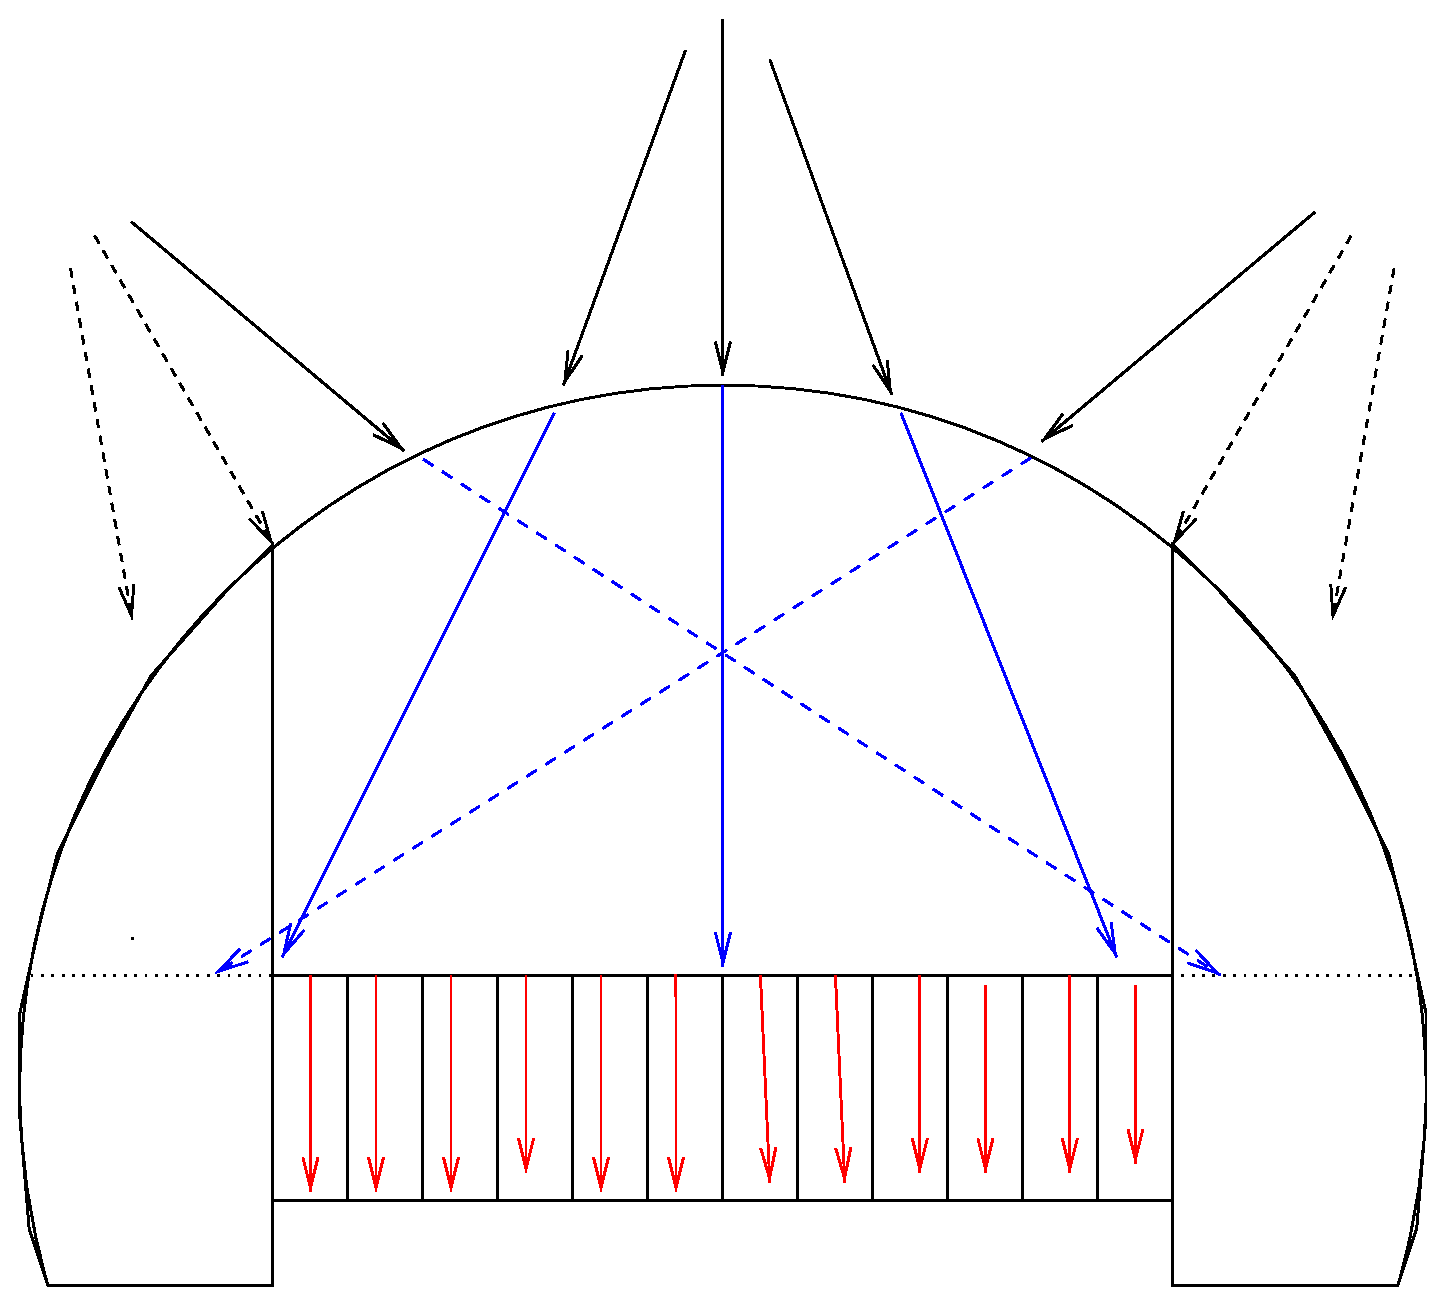
\includegraphics[height=5cm]{./figures/FCAlgo.eps}
&
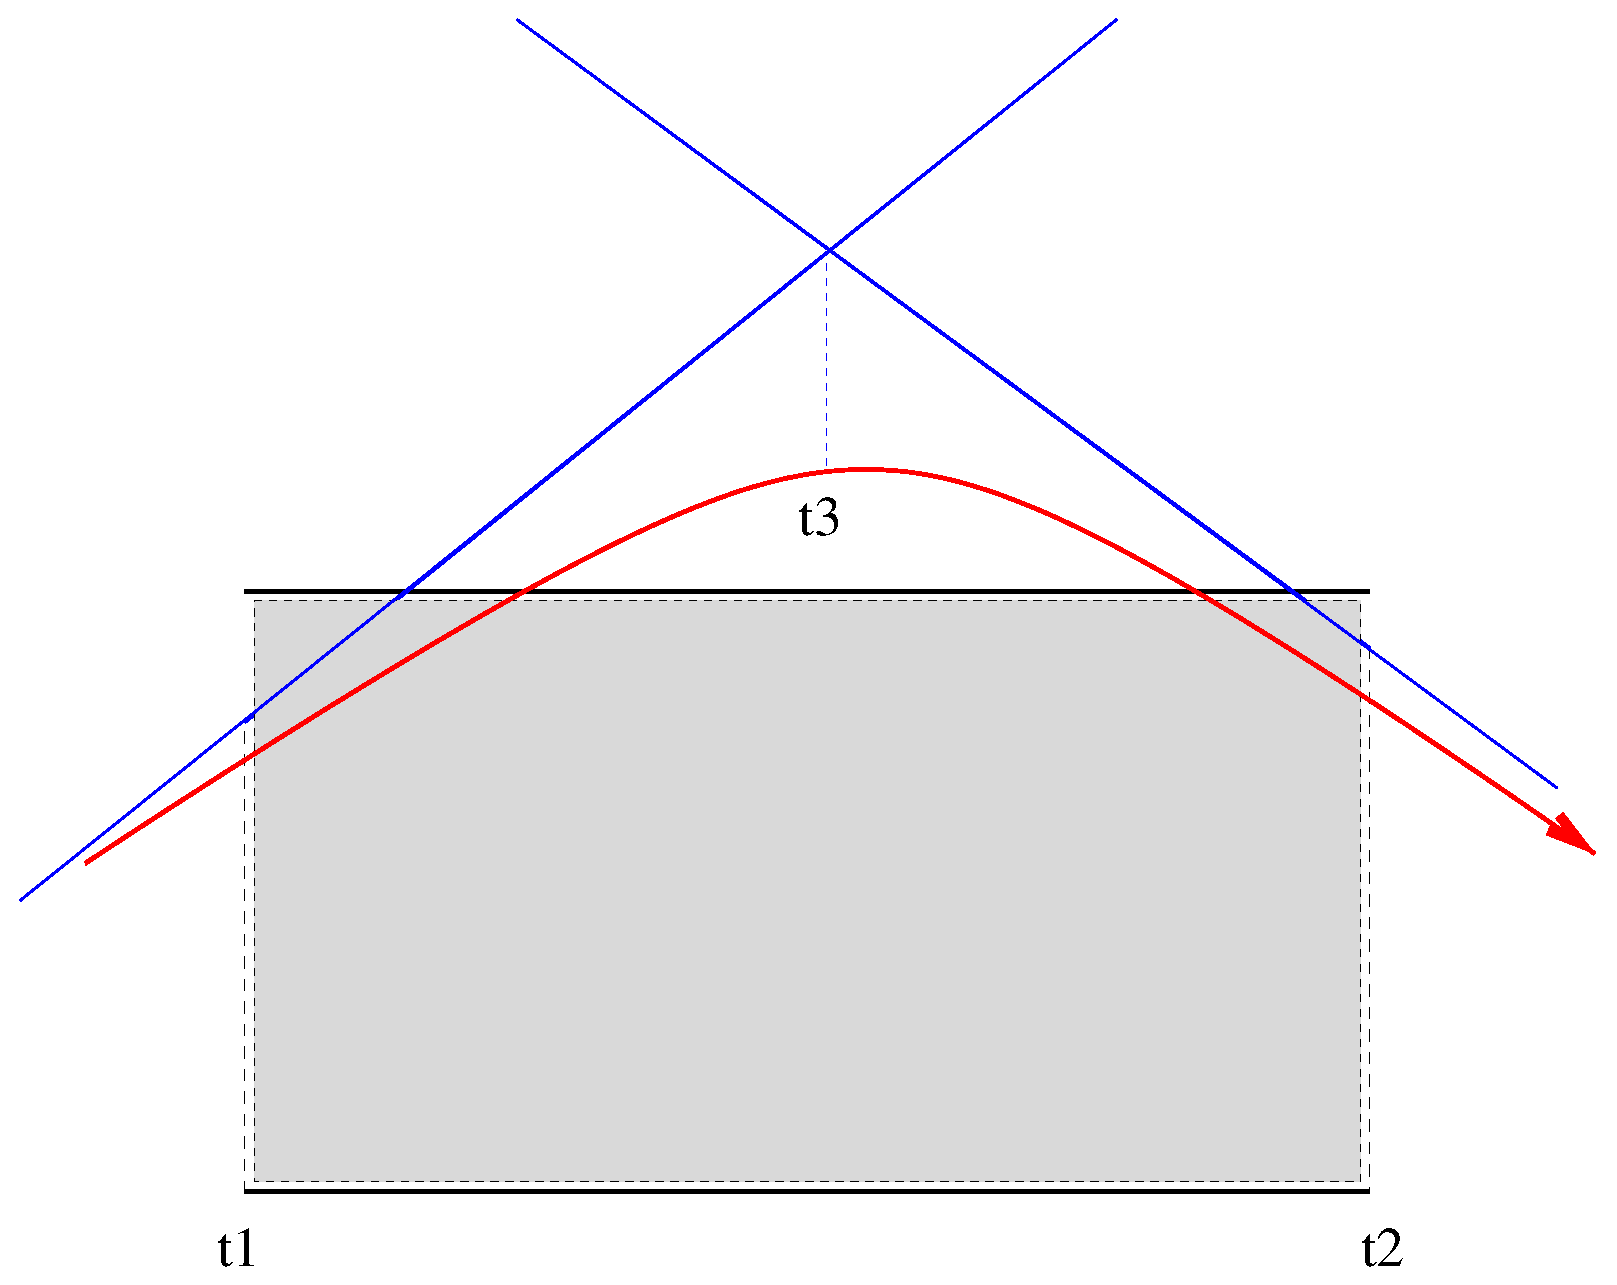
\includegraphics[height=5cm]{./figures/FCtangents.eps}
\end{tabular}
\end{center}
\caption{The different steps in the algorithm (left). A neutron trajectory in a slit (right)}
\label{fig:TOFalg.eps}
\end{figure}

The neutrons are first propagated to the outer chopper cylinder and their coordinates are transformed into the rotating frame using $T$. Neutrons outside the slit channel (chopper opening), or hitting the top and bottom caps are absorbed (yellow dots in Fig. \ref{fig:Overview.eps}). The side from which the neutron approaches the chopper is known (positive or negative z'-axis of the rotating frame) so that the calculation of the time of interaction with the slit package entrance $t_1$ is performed solving $z' = \pm \frac{\rm length}{2}$ in Eq. (\ref{eq:Txz}). Using the result of the numerical algorithms the neutron propagates to the entrance of the slit package (orange circles in Fig. \ref{fig:Overview.eps}). Neutrons getting aside the slit package entrance are absorbed. Additionally, the slit package exit time $t_2$ is estimated the same way with $z' = \mp \frac{\rm length}{2}$, in order to evaluate the whole time-of-flight in the chopper. The index of the slit which was hit is also computed, as we know the $x'$ coordinate in the rotating frame at the slit entrance.

Differentiating Eq. (\ref{eq:Txz}) for $x$ coordinate
\begin{equation}
\dot{x'}(t) = v_x'(t) = [v_x+\omega.(z+v_z(t))]\cos(\omega(t-t_0))
+ [v_z-\omega.(x+v_x(t))]\sin(\omega(t-t_0))
\end{equation}
we may estimate the tangents to the spiral neutron trajectory in the rotating frame at times $t_1$ and $t_2$. The intersection of these two lines gives an intermediate time $t_3$.

If the neutron remains in the same slit at this point, then there is no intersection with the slit walls (direct flight), and the neutron may be propagated to the slit output, and then to the cylinder output. A last check is made for the neutron to pass the chopper aperture in the cylinder.

If the neutron changes of slit channel at this point, we may determine the intersection time of the neutron trajectory within $[ t_1, t_3 ]$ or $[ t_3, t_2 ]$, as seen in Fig. \ref{fig:TOFalg.eps}. If walls are not reflecting, we just absorb neutrons here.

\subsubsection{The reflections (super-mirror slits)}

If slit walls are reflecting, neutron is first propagated to the slit separating surface. Then the velocity in the rotating frame is computed using Eq. (\ref{eq:Txz}). Perpendicular velocity $v_x'$ is reverted for reflection, and inverse $T$ transformation is performed. Reflected intensity is computed the same way as for the guide component (see section \ref{s:mirror}). The remaining time $t_2$ to the slit output is estimated and the tangent intersection process is iterated, until neutron exits.

The propagation is finalized when determining the intersection of the neutron trajectory with the outer surface of the chopper cylinder. The neutron must then pass its aperture, else it is absorbed.

\subsubsection{Curved slit packages}

The effect of curvature can significantly improve the flux and energy resolution shape for thermal and hot neutrons.

As all $(xz)$ cordinates are transformed into $(x'z')$, the most efficient way to take into account the curvature is to include it in the transformation by 'morphing' the curved rotating real space to a straight still frame. Then instead of solving
\begin{equation}x'(t) = d +\Delta_{x'}(z') {\rm\ where\ } \Delta_{x'}(z')=R_{slit}.(1-\sqrt{1-(z'/R_{slit})^2})
\end{equation}
with $\Delta$ being the gap between the straight tangent line at the slit center and the real slit shape, we perform the additional transformation
\begin{equation}
x' \rightarrow x' - \Delta_{x'}(z')
\end{equation}
The additional transformation counter-balance the real curvature so that the rest of the algorithm is written as if slits were straight.
This applies to all computations in the rotating frame, and thus as well to reflections on super mirror coatings.


% Emacs settings: -*-mode: latex; TeX-master: "manual.tex"; -*-

\section{Vitess\_ChopperFermi: The Fermi Chopper from Vitess}
\label{s:vit_fc}

\component{Vitess\_ChopperFermi}{Geza Zsigmond}{GeomOption, $N_{\rm chan}$, $f$, $h$, $w_{\rm tot}$, $l$, $r_{\rm curv}$, $d$, $\phi$, $w_{\rm wall}$, GeomFile}{zerotime, $N_{\rm gates}$}{validated}


The component {\bf Vitess\_ChopperFermi} simulates a Fermi chopper with absorbing walls.
The shape of the channels can be straight, curved with circular, or curved with ideal
(i.e. close to a parabolic) shape.
This is determined by the parameter 'GeomOption'. In the option 'straight Fermi
chopper', the very fast neutrons are transmitted with only a time modulation and lower
speed neutrons are modulated both in time of flight and wavelength.
If the channels are curved, the highest transmission occurs for a wavelength

\begin{equation}
\lambda_{\rm opt} = \frac{3956 {\rm [m\AA/s]}}{2 \omega r_{\rm curv}}
\end{equation}

with

\begin{equation}
\omega = 2 \pi f
\end{equation}

The optimal shape is calculated in an exact way and is close to parabolic; in this
case, transmission is as high for the optimal wavelength as in the case of a straight
Fermi chopper for the limit $\lambda \rightarrow 0$.
In the more realistic case of circular shapes channels, the transmission is slightly
lower. In general, neutrons are transmitted through a curved Fermi chopper with a time
AND wavelength modulation .

The rotation axis is vertical (y-axis), i.e. the path length through the channels is
given by the length $l$ along the z-axis. The inital orientation is given by the phase
$\phi$ of the chopper - $\phi$ = 0 means transmission orientation.

Geometry for {\bf straight} and {\bf circular} channels:
The geometry of the chopper consists of a rectangular shaped object with a channel
system. In transmission position, there are $N_{\rm gates}$ slits of width $w_{\rm slit}$
each along the x-axis, separated by absorbing walls of thickness $w_{\rm wall}$
(see figure~\ref{f:vit_fc1}). The total width $w_{\rm tot}$ is given by

\begin{equation}
w_{\rm tot} = N_{\rm gates} w_{\rm slit} + (N_{\rm gates}+1) w_{\rm wall}
\end{equation}

The rectangular channel system is surrounded by a so-called shadowing cylinder; it is a
part of a cylinder with vertical symmetry axis and diameter

\begin{equation}
d \geq \sqrt{l^2 + w_{\rm tot}^2}
\end{equation}

It serves to prevent transmission of neutrons which do not fly through the channels;
but it also reduces the transmission, because the cylinder removes neutrons
in front of the channel entrance or behind the channel exit (see figure~\ref{f:vit_fc1}).

\begin{figure}[ht]
\begin{center}
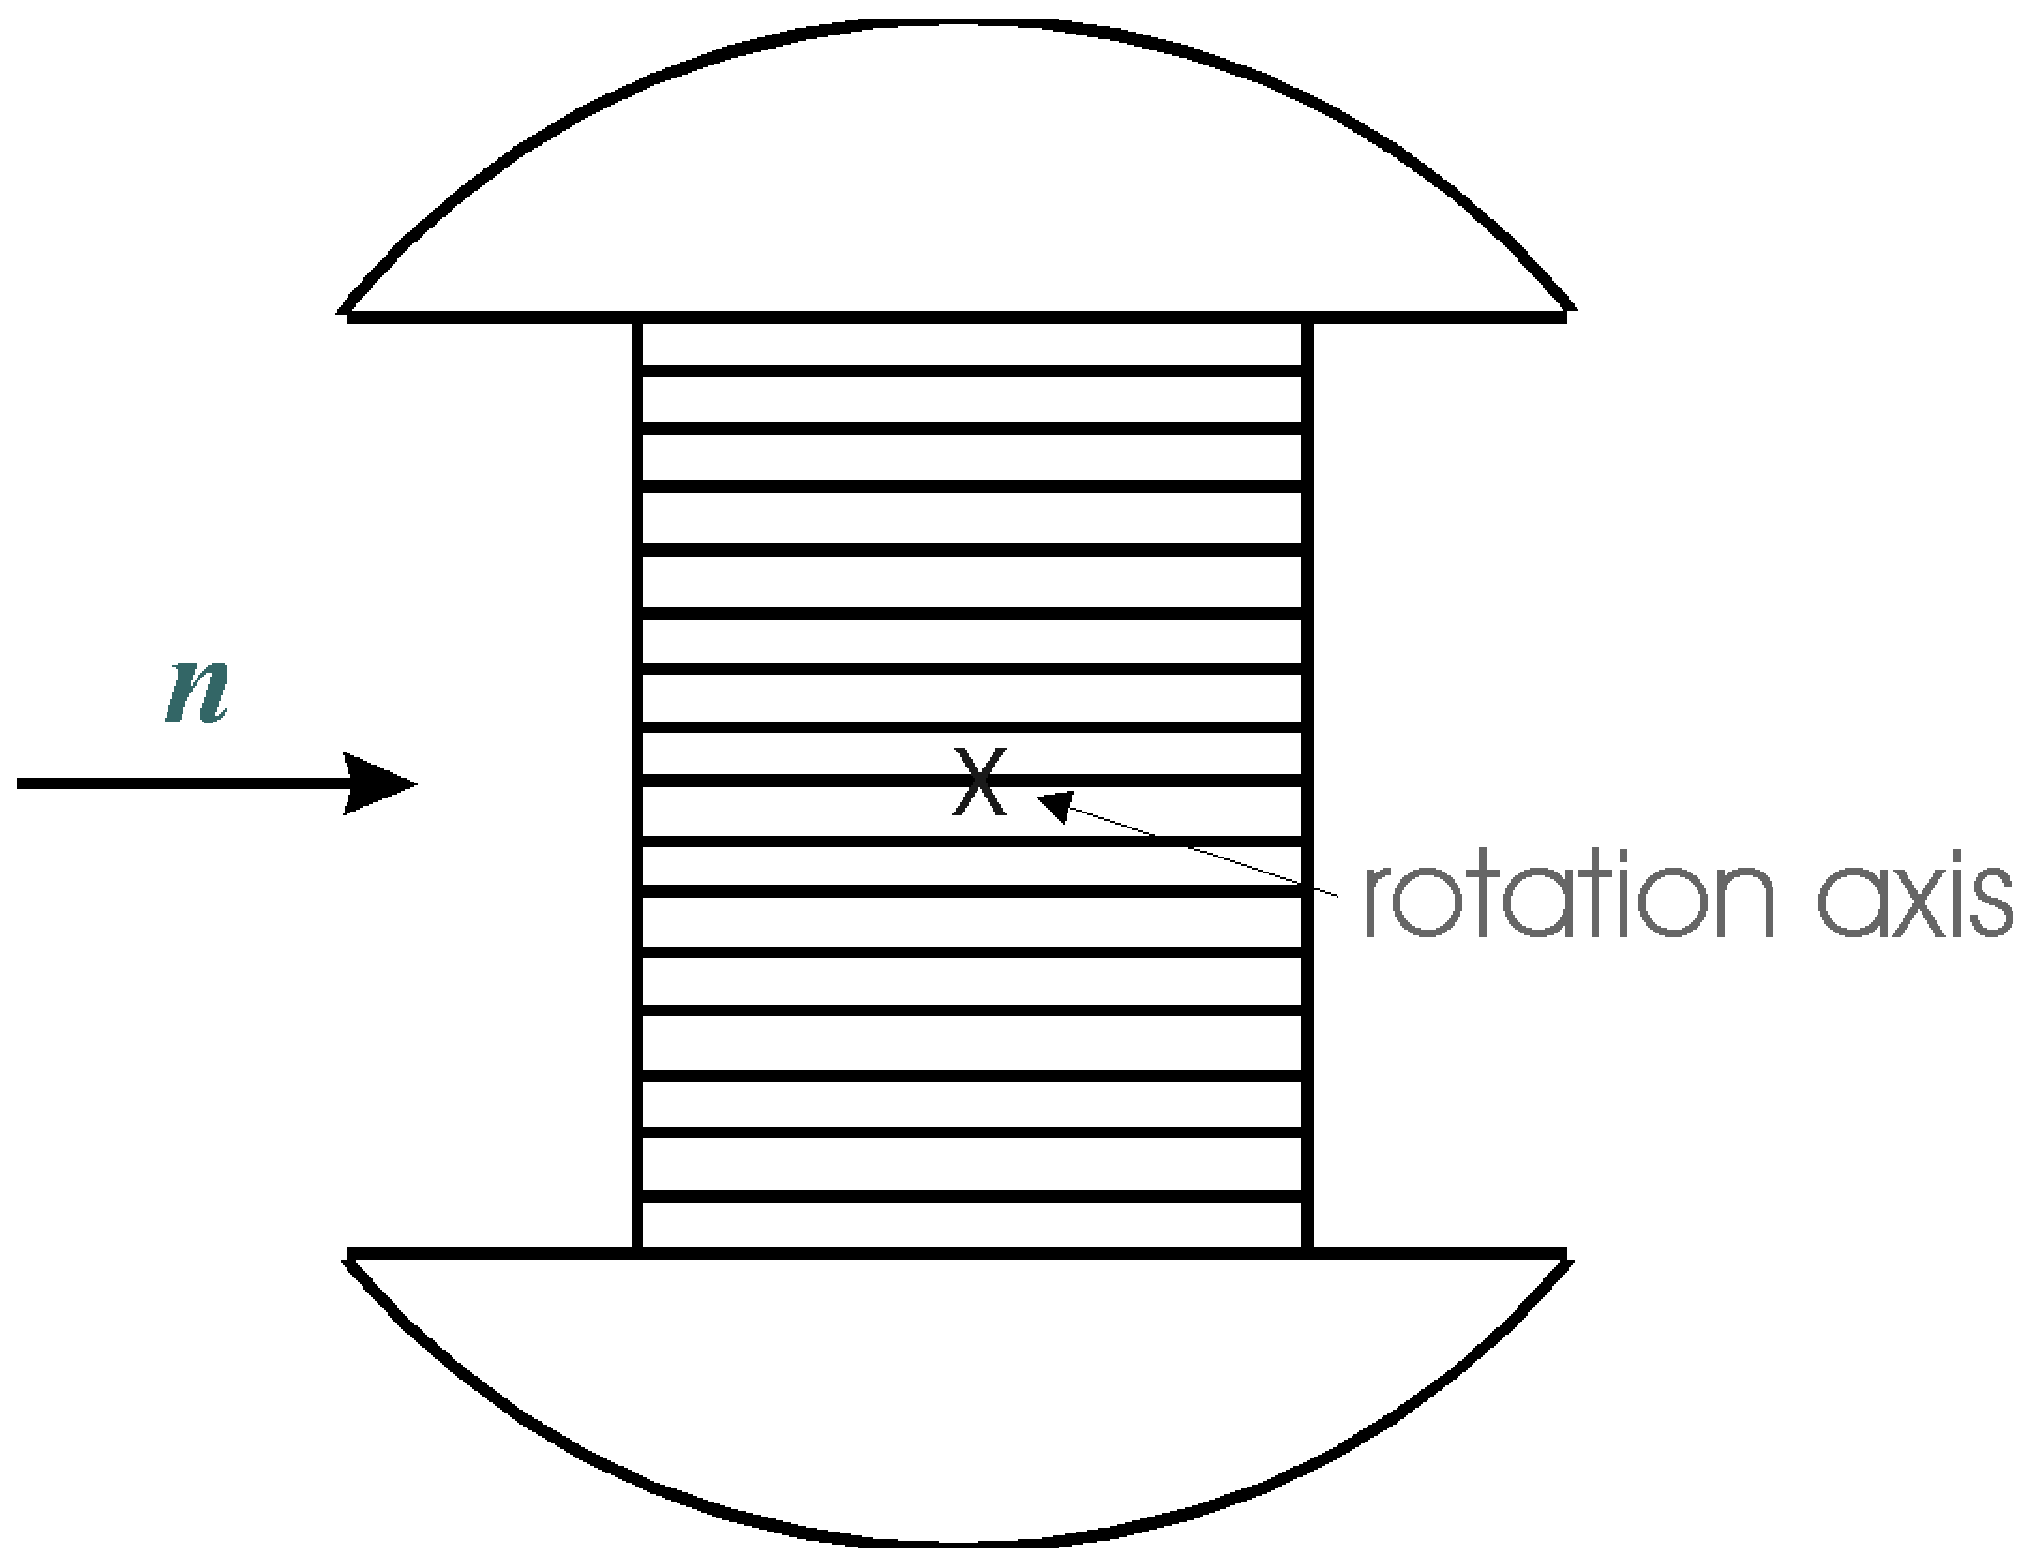
\includegraphics[width=0.45\linewidth]{figures/vitess_fc_str.eps}
\caption{geometry of a staight Fermi chopper\label{f:vit_fc1}}
\end{center}
\end{figure}

Geometry for {\bf parabolic} channels:
In this case, the Fermi chopper is supposed to be a full cylinder, i.e. the central
channels are longer than those on the edges. The other features are the same as for
the other options. (see figure~\ref{f:vit_fc2}).

\begin{figure}[ht]
\begin{center}
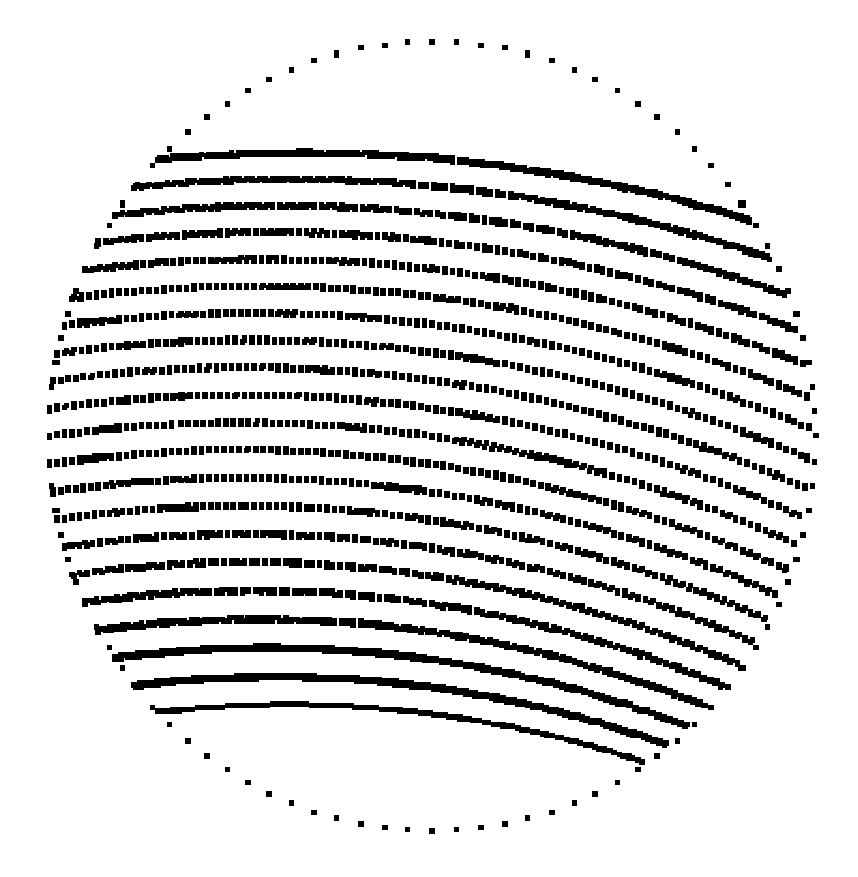
\includegraphics[width=0.4\linewidth]{figures/vitess_fc_parab.eps}
\caption{geometry of a curved Fermi chopper\label{f:vit_fc2}}
\end{center}
\end{figure}

The algorithm works with a rotating chopper framework. Neutrons hitting the channel
walls are absorbed. The channels are approximated by $N_{\rm gates}$ gates. If the trajectory
takes a course through all the gates, the neutron passes the Fermi chopper. There are gates at
the entrance and the exit of the channel. The other gates are situated close to the centre of
the Fermic chopper.
Precision of the simulation increases with the number of gates, but also the computing time needed.
The use of four channels already gives exact transmission shapes for lower wavelengths
($\lambda < 6$ \AA) and good approximation for higher ones. It is recommended to use larger number of
channels only for a check.

The option 'zerotime' may be used to reset the time at the chopper position. The time is
set to a value between -$T_{\rm p}$/2 and +$T_{\rm p}$/2 (with $T_{\rm p}$ being the maximal pulse length),
depending on the phase of the chopper at the moment of passing the chopper centre. The
result is the generation of only 1 pulse instead of several; this is useful for TOF instruments
on continuous sources.


\newpage
\section{V\_selector: A rotating velocity selector}
\label{vselector}
\index{Optics!Velocity selector}

\component{V\_selector}{System}{$L_0$, $L_1$, $\omega$, $r_0$, $\phi$, $N$}{}{validated, position is center of input aperture}

\begin{figure}
  \begin{center}
    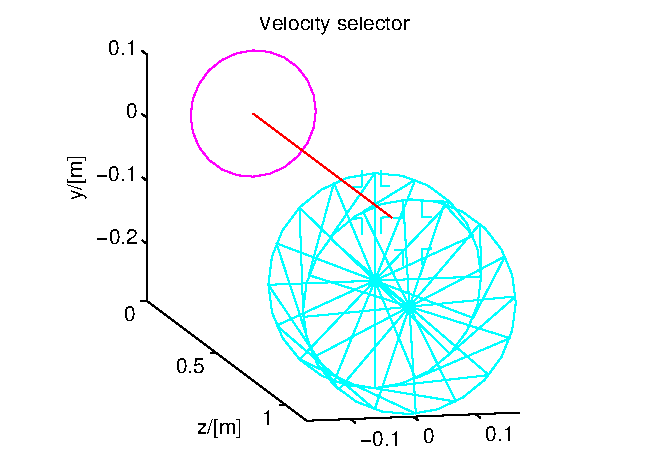
\includegraphics[width=0.9\textwidth]{figures/vselector.eps}
  \end{center}
\caption{A velocity selector}
\label{f:vselector}
\end{figure}

The component {\bf V\_selector} models a rotating velocity
selector constructed from $N$ collimator blades
arranged radially on an axis. Two identical slits ($height \times width$)
at a 12 o'clock position allow
neutron passage at the position of the blades.
The blades are "twisted" on the axis so that a stationary
velocity selector does not transmit neutrons; the total
twist angle is denoted $\phi$ (in degrees).

Further input parameters for {\bf V\_selector} 
the distance between apertures, $L_0$, the length of the
collimator blades, $L_1$, the height from rotation axix to the slit
centre, $r_0$, the rotation speed $\omega$ (in rpm), 
and the blade thickness $t$.

The local coordinate system is centered at the slit centre.

The component {\rm Selector} produces equivalent results.

\subsection{Velocity selector transmission}
By rotating the selector you allow
transmittance of neutrons rays with velocities around a mean value, given by
\begin{equation}
V_0 = \omega L / \phi ,
\end{equation}
which means that the selector has turned the twist angle
$\phi$ during the typical neutron flight time $L/V_0$.

Neutrons having a velocity slightly different from $V_0$
will either be transmitted or absorbed depending on the exact position
of the rotator blades when the neutron enters the selector.
Assuming this position to be unknown and integrating over all possible
positions (assuming zero thickness of blades), we arrive at a transmission factor
\begin{equation}
T = \left\{
 \begin{array}{ll}
 1 - (N/2\pi ) |\phi-\omega L / V| &
        {\rm if}\;   (N/2\pi )|\phi -\omega L / V| < 1 \\
    0  &  {\rm otherwise}
 \end{array} \right.
\end{equation}
where $N$ is the number of collimator blades.

A horisontal divergence changes the above formula because of the
angular difference between the entry and exit points of the neutron.
The resulting transmittance resembles the one above, only with
$V$ replaced by $V_z$ and $\phi$ replaced by $(\phi +\psi )$,
where $\psi$ is the angular difference due to
the divergence. An additional vertical divergence does not change
this formula, but it may contribute to $\psi$.
(We have here ignored the very small non-linearity of $\psi$ along the
neutron path in case of both vertical and horisontal divergence).

Adding the effect of a finite blade thickness, $t$, reduces the transmission
by the overall factor
\begin{equation}
\left( 1-\frac{N t}{2\pi r}  \right),
\end{equation}
where $r$ is the distance from the rotation axis. We ignore the variation
of $r$ along the neutron path and use just the average value.




% there follows a chapter
\newpage
% Emacs settings: -*-mode: latex; TeX-master: "manual.tex"; -*-

\chapter{Monochromators}

In this class of components, we are concerned with elastic Bragg
scattering from monochromators. {\bf Monochromator\_flat} 
models a flat thin mosaic crystal with a single scattering vector
perpendicular to the surface.  
The component {\bf Monochromator\_curved} is similar, 
but models a singly or doubly bend monochromator crystal arrangement.

A much more general model of scattering from a single crystal is 
found in the component {\bf Single\_crystal},
which is presented under Samples, chapter~\ref{c:samples}.

\section{Monochromator\_flat: An infinitely thin, flat mosaic crystal with
a single scattering vector}
\label{s:monochromator_flat}
\index{Optics!Monochromator}

\component{Monochromator\_flat}{System}{$z_{\rm min}$, $z_{\rm max}$, $y_{\rm min}$, $y_{\rm max}$, $\eta_{\rm h}$, $\eta_{\rm v}$, $R_0$, $Q_0$}{$d_{\rm m}$}{In reflecting geometry, non polarized}

This component simulates an infinitely thin single
crystal with a single scattering vector, $Q_0=2\pi / d_m$, perpendicular to the
surface. A typical
use for this component is to simulate a simple monochromator or analyzer.

The monochromator dimensions are given by the length, $z_{\rm w}$, and
the height, $y_{\rm h}$. As the parameter names indicate, the
monochromator is placed in the $z-y$ plane of the local coordinate system.
This definition is made to ensure that the physical monochromator angle
(often denoted \verb+A1+) will equal the \MCX\ rotation angle
of the Monochromator component around the $y$-axis.
$R_0$ is the maximal reflectivity and
$\eta_{\rm h}$ and $\eta_{\rm v}$ are the horizontal and vertical mosaicities,
respectively, see explanation below.

\subsection{Monochromator physics and algorithm}
The physical model used in {\bf Monochromator\_flat} is a rectangular piece of
material composed of a large number of small micro-crystals.
The orientation of the
micro-crystals deviates from the nominal crystal orientation so that the
probability of a given micro-crystal orientation is proportional to a
Gaussian in the angle between the given and the nominal orientation. The
width of the Gaussian is given by the mosaic spread, $\eta$, of the crystal
(given in units of arc minutes).
$\eta$ is assumed to be large compared to the inherent Bragg width of the
scattering vector (often a few arc seconds).
(The mosaicity gives rise to a Gaussian reflectivity profile of width
similar to - but not equal - the intrinsic mosaicity.
In this component, and in real life, the mosaicity given is that of the
reflectivity signal.)

As a further simplification, the crystal is assumed to be infinitely
thin. This means that multiple scattering effects are not simulated. It
also means that the total reflectivity, $r_0$ is used as a parameter for
the model rather than the atomic scattering cross section, implying that
the scattering efficiency does not vary with neutron wavelength.
The variance
of the lattice spacing ($\Delta d/d$) is assumed to be zero, so this
component is not suitable for simulating backscattering instruments (use
the component {\rm Single\_crystal}
in section~\ref{s:Single_crystal} for that).

When a neutron trajectory intersects the crystal, the first step in the
computation is to determine the probability of scattering. This
probability is then used in a Monte Carlo choice deciding whether to
scatter or transmit the neutron. The physical scattering probability is the sum
of the probabilities of first- second-, and higher-order scattering -
up to the highest order possible for the given neutron wavelength.
However, in most cases at most one order will have a
significant scattering probability, and the computation thus considers
only the order that best matches the neutron wavelength.

The scattering of neutrons from a crystal is governed by Bragg's law:
\begin{equation}
n{\bf Q}_0 = 2{\bf k}_i\sin\theta
\end{equation}
The scattering order is specified by the integer $n$. We seek only one
value of $n$, namely the one which makes
$n {\bf Q}_0$ closest to the projection of $2{\bf k}_i$ onto ${\bf Q}_0$
(see figure~\ref{f:mosaic_order}).
%  k=2PI/lambda
%  q=2k sin(theta)
%
%  2 PI n/k = d q/2k
%  q = n 4 PI/d
%
%  n 2PI/k = n 4 PI/q \sin\theta
%  1/k = 2/q\sin\theta
%  n q = 2k\sin\theta
\begin{figure}
  \begin{center}
    \psfrag{theta}[l][l]{$\theta$}
    \psfrag{ki}[r][r]{$2{\bf k}_{\rm i}$}
    \psfrag{Q0}[l][l]{${\bf Q}_0$}
    \psfrag{2Q0}[l][l]{$2{\bf Q}_0$}
    \psfrag{3Q0}[l][l]{$3{\bf Q}_0$}
    \psfrag{4Q0}[l][l]{$4{\bf Q}_0$}
    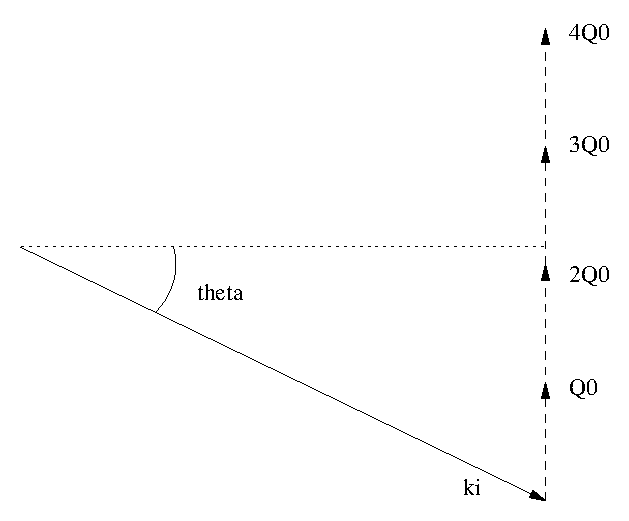
\includegraphics[width=0.5\textwidth]{figures/mosaic_order.eps}
  \end{center}
\caption{Selection of the Bragg order (``2'' in this case).}
\label{f:mosaic_order}
\end{figure}
%

Once $n$ has been determined, the Bragg angle $\theta$ can be
computed. The angle $\alpha$ is the amount one would need to
turn the nominal scattering vector ${\bf Q}_0$ for the monochromator
to be in Bragg scattering condition.
We now use $\alpha$ to compute the probability of reflection from
the mosaic crystal
\begin{equation}
p_{\rm reflect} = R_0 e^{-\alpha^2/2\eta^2},
\end{equation}
The probability $p_{\rm reflect}$ is used
in a Monte Carlo choice to decide whether the neutron is transmitted or
reflected.
%
%\begin{figure}
%  \begin{center}
%    \psfrag{th}[r][r]{$\theta$}
%    \psfrag{ki}[r][r]{$2{\bf k}_{\rm i}$}
%    \psfrag{kf}[l][l]{$2{\bf k}_{\rm f}$}
%    \psfrag{Q0}[l][l]{${\bf Q}_0$}
%    \psfrag{alpha}[c][c]{$\alpha$}
%    \psfrag{q}[l][l]{$\bf q$}
%    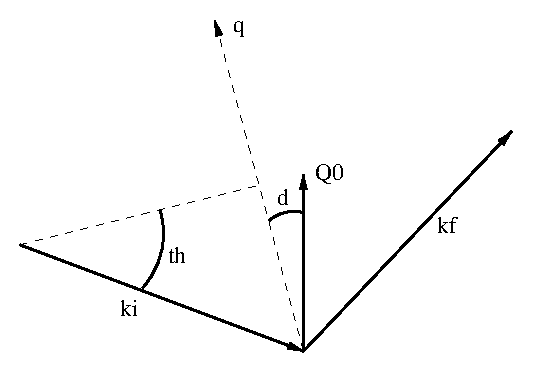
\includegraphics[width=0.5\textwidth]{figures/mosaic_angle.eps}
%  \end{center}
%\caption{Computing the deviation $d$ from the nominal scattering direction.}
%\label{f:mosaic_angle}
%\end{figure}

In the case of reflection, the neutron will be scattered into the
Debye-Scherrer cone, with the probability of each point on the cone
being determined by the mosaic. The Debye-Scherrer cone can be described
by the equation
\begin{equation}
  \label{eq:mosaic_cone}
  {\bf k}_{\rm f} = {\bf k}_{\rm i}\cos2\theta +
      \sin2\theta({\bf c}\cos\varphi + {\bf b}\sin\varphi),
      \qquad\varphi\in[-\pi;\pi],
\end{equation}
where ${\bf b}$ is a vector perpendicular to ${\bf k}_{\rm i}$ and ${\bf
Q}_0$, ${\bf c}$ is perpendicular to ${\bf k}_{\rm i}$ and ${\bf b}$,
and both ${\bf b}$ and ${\bf c}$ have the same length as ${\bf k}_{\rm i}$
(see figure~\ref{f:mosaic_cone}). When choosing $\varphi$ (and
thereby ${\bf k}_{\rm f}$), only a small part of the full $[-\pi; \pi]$
range will have appreciable scattering probability in non-backscattering
configurations. The best statistics is thus obtained by sampling
$\varphi$ only from a suitably narrow range.

The (small) deviation angle $\alpha$ of the nominal
scattering vector $n{\bf Q}_0$ corresponds to a $\Delta q$ of
\begin{equation}
\Delta q \approx \alpha 2k\sin\theta.
\end{equation}
The angle $\varphi$ corresponds to a $\Delta k_{\rm f}$ (and hence
$\Delta q$) of
\begin{equation}
\Delta q \approx \varphi k \sin(2\theta)
\end{equation}
(see figure~\ref{f:mosaic_cone}).
Hence we may sample $\varphi$ from a Gaussian with standard deviation
\begin{equation}
\alpha\frac{2k\sin\theta}{k\sin(2\theta)} =
\alpha\frac{2k\sin\theta}{2k\sin\theta\cos\theta} =
\frac{\alpha}{\cos\theta}
\end{equation}
to get good statistics.
%
\begin{figure}
  \begin{center}
    \psfrag{th}[r][r]{$2\theta$}
    \psfrag{ki}[c][c]{$2{\bf k}_{\rm i}$}
    \psfrag{kf}[r][r]{$2{\bf k}_{\rm f}$}
    \psfrag{nQ0}[l][l]{$n{\bf Q}_0$}
    \psfrag{q}[l][l]{$\bf q$}
    \psfrag{2ksin2t}[l][l]{$2 k \sin(2 \theta)$}
    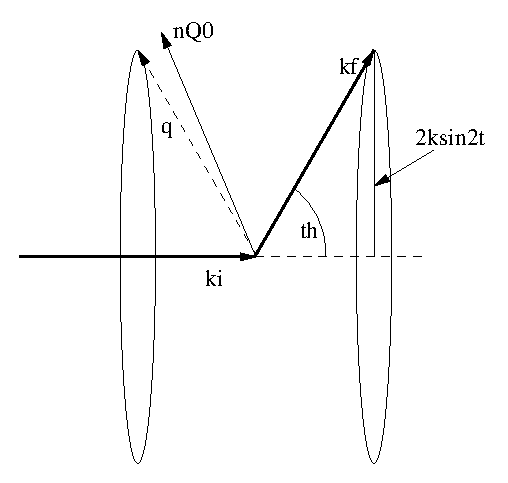
\includegraphics[width=0.5\textwidth]{figures/mosaic_cone.eps}
  \end{center}
\caption{Scattering into the part of the Debye-Scherrer cone covered by
    the mosaic.}
\label{f:mosaic_cone}
\end{figure}

What remains is to determine the neutron weight. The distribution from
which the scattering event is sampled is a Gaussian in $\varphi$ of
width $\frac{\alpha}{\cos\theta}$,
\begin{equation}
    f_{\rm MC}(\varphi) = \frac{1}{\sqrt{2\pi}(\sigma/\cos\theta)}
            e^{-\varphi^2/2(\sigma/\cos\theta)^2}
\end{equation}
In the physical model, the probability of the scattering event is
proportional to a Gaussian in the angle between the nominal scattering
vector ${\bf Q}_0$ and the actual scattering vector ${\bf q}$. The
normalization condition is that the integral over all $\varphi$ should
be 1. Thus the probability of the scattering event in the physical model
is
\begin{equation}
  \label{eq:mosaic_integral}
  \Pi(\varphi) = e^{\frac{-d(\varphi)^2}{2\sigma^2}} /
   \int_{-\pi}^{\pi} e^{\frac{-d(\varphi)^2}{2\sigma^2}} d\varphi
\end{equation}
where $d(\varphi)$ denotes the angle between the nominal scattering
vector and the actual scattering vector corresponding to $\varphi$.
According to equation~(\ref{probrule}), the weight adjustment $\pi_j$ is
then given by
\begin{equation}
\pi_j = \Pi(\varphi) / f_{\rm MC}(\varphi).
\end{equation}
In the implementation, the integral in~(\ref{eq:mosaic_integral}) is computed
using a 15-order Gaussian quadrature formula, with the integral
restricted to an interval of width $5\sigma/\cos\theta$ for the same
reasons discussed above on the sampling of $\varphi$.

\newpage
% Emacs settings: -*-mode: latex; TeX-master: "manual.tex"; -*-

\section{Monochromator\_curved: An infinitely thin, curved mosaic crystal with
a single scattering vector}
\label{s:monochromator_curved}
\index{Optics!Monochromator, curved}

\component{Monochromator\_curved}{(System) Peter Link, FRM-2}{$z_{\rm w}$, $y_{\rm h}$, gap, $\eta_{\rm h}$, $\eta_{\rm v}$, $n_{\rm h}$, $n_{\rm v}$, $R_0$, $Q$, $r_{\rm h}$, $r_{\rm v}$}{$d_{\rm m}$, $\eta$, $h$, $w$, verbose, transmit, reflect}{}

\begin{figure}
  \begin{center}
    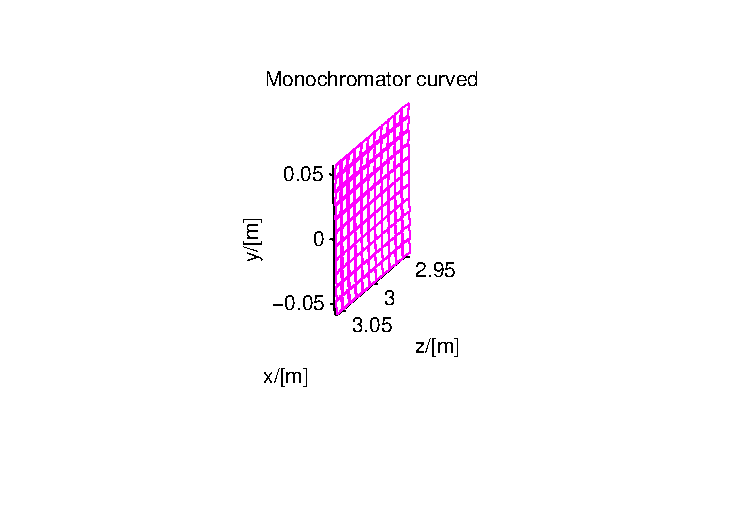
\includegraphics[width=0.9\textwidth]{figures/monochromator_curved.eps}
  \end{center}
\caption{A curved monochromator}
\label{f:monochromator_curved}
\end{figure}


This component simulates an array of infinitely thin single
crystals with a single scattering vector perpendicular to the
surface and a mosaic spread.
This component is used to simulate a singly or doubly
curved monochromator or analyzer, in reflecting geometry.

The component uses  rectangular pieces of monochromator material
as described in {\bf Monochromator\_curved}.
The scattering vector is named $Q$, and as described in
{\bf Monochromator\_flat}, multiples of $Q$ can be applied.
Other important parameters are the piece height and width,
$y_{\rm h}$ and $z_{\rm w}$, respectively, the
horizontal and vertical mosaicities, $\eta_{\rm h}$ and $\eta_{\rm v}$,
respectively. 
If just one mosaicity, $\eta$, is specified, this the same for both directions.

The number of pieces vertically and horizontally are called
$n_{\rm v}$ and $n_{\rm h}$, respectively, and the vertical and horizontal
radii of curvature are named $r_{\rm v}$ and $r_{\rm h}$, respectively.
All single crystals are positioned in the same vertical plane, 
but tilted accordingly to the curvature radius.

The constant monochromator reflectivity, $R_0$ can be replaced by
a file of tabulated reflectivities. In the same sense, the transmission
can be modeled by a tabulated file (for non reflected neutrons).

As for {\bf Monochromator\_flat}, the crystal is assumed to be infinitely
thin, and the varition in lattice spacing, ($\Delta d/d$),
is assumed to be zero. Hence, this
component is not suitable for simulating backscattering instruments or to
investigate multiple scattering effects.

The algorithm for scattering and calculation of the neutron weight for
the individual blades is described under {\bf Monochromator\_flat}.




\chapter{Samples}
\index{Library!Components!samples}
\index{Samples|textbf}
\label{c:samples}

This class of components models the sample of the experiment.
This is by far the most challenging part of a neutron scattering
instrument to model. However, for purpose of simulating
instrument performance, details of the samples are rather unimportant,
allowing for simple approximations. On the contrary, for full
virtual experiments it is of importance to have realistic and
detailed sample descriptions. \MCS\ contains both simple and detailed
samples, although there is still room for much more development.

We first consider incoherent scattering. The simple component {\bf Vanadium}
performs both incoherent scattering and absorption.

An important component class is elastic Bragg scattering from an ideal powder.
The component {\bf PowderN} models a powder scatterer with reflections
given in a LAZY / Crystallographica file.
The component includes absorption and incoherent scattering.

Next type is Bragg scattering from single crystals.
The simplest single crystals are in fact the monochromator components
{\bf Monochromator\_flat} and {\bf Monochromator\_curved},
which were presented in the section on optics.
The monochromators are models of a thin mosaic crystal
with a single scattering vector perpendicular to the surface.
Much more advanced, the component {\bf Single\_crystal}
is a general single crystal sample (with multiple scattering) that allows
the input of an arbitrary unit cell and a list of structure factors, read
from a LAZY / Crystallographica file.
This component also allows anisotropic mosaicity
and $\Delta d/d$ lattice space variation.

Isotropoic small-angle scattering is simulated in {\bf Sans\_Spheres},
which models scattering from a collection of hard spheres. A more general
SANS sample is under development.
In addition, a reflectometry sample will soon be developed.

Inelastic scattering from a dispersion is exemplified by
the component {\bf Phonon\_simple}, which models a single phonon dispersion.

For a more general sample model, the {\bf Isotropic\_Sqw} component
is able to simulate all kinds of isotropic materials:
Liquids, glasses, polymers, powders, etc, with $S(q,\omega)$ table
specified by an input file.
Physical processes include coherent/incoherent scattering,
both elastic and inelastic, with absorption and multiple scattering.
Moreover, this component may be used concentrically,
to model a sample environment.
Thus it may handle most samples except single crystals.

In general, all samples are assumed to be homogeneous. There would also be
potential in developing an inhomogeneous sample, e.g. with
spatially varying lattice constant, relevant for stress/strain scanners.
Inhomogeneously absorbing sample for tomography could also be possible.
Further, no polarization effects are yet taken into account in any
of the samples.

\begin{table}
  \begin{center}
  {\let\my=\\
    \begin{tabular}{|c|cc|cc|c|c|}
    \hline
    Sample        & \multicolumn{2}{c|}{Coherent} & \multicolumn{2}{c|}{Incoherent} &&\\
    Process       & Elastic & Inelastic & Elastic & Inelastic & Absorption & Multi. Scatt.\\
    \hline
    Phonon\_simple&         & X         &         &           & X & \\
    Isotropic\_Sqw&  X      & X         & X       & X         & X & X \\
    PowderN       &  N lines&           &         &           & X & \\
    Sans\_spheres &  colloid&           &         &           & X & \\
    Single\_crystal& X      &           & X       &           & X & X \\
    V\_sample     &         &           & X       &           & X & \\
    \hline
    \end{tabular}
    \caption{Processes implemented in sample components}
    \label{t:sample-process}
  }
  \end{center}
\end{table}

\section{V\_sample: An incoherent scatterer, the V-sample}
\label{s:v_sample}
\index{Samples!Incoherent isotropic scatterer (Vanadium)}
\index{Incoherent elastic scattering}

\component{V\_sample}{System}{$r_{\rm i}$, $r_{\rm o}$, $h$, $r_{\rm foc}$, $x_{\rm target}$, $y_{\rm target}$, $z_{\rm target}$}{$w_x$, $h_y$, $t_z$, $w_{\rm focus}, h_{\rm focus}$, $w_{\rm foc, angle}$, $h_{\rm foc, angle}$, \\ $\sigma_{\rm abs}$, $\sigma_{\rm inc}$, $V_0$, $f_{\rm pack}$, target\_index}{validated}

A sample with incoherent scattering, e.g. vanadium, is frequently used for
calibration purposes, as this gives an isotropic, elastically scattered beam.

The component {\bf V\_sample}
has {\em only} absorption and incoherent scattering.
For the sample geometry, we default use a
hollow cylinder (which has the solid cylinder as a limiting case).
The sample dimensions are: Inner radius $r_{\rm i}$,
outer radius $r_{\rm o}$, and height $h$, see figure \ref{f:v-sample}.
\begin{figure}
  \begin{center}
    \psfrag{ri}{$r_i$}
    \psfrag{ro}{$r_o$}
    \psfrag{h}{$h$}
    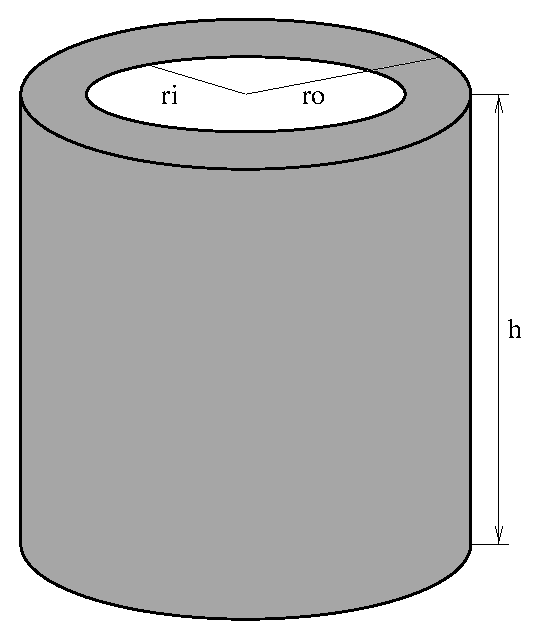
\includegraphics[width=0.3\textwidth]{figures/vsample.eps}
  \end{center}
\caption{The geometry of the hollow-cylinder vanadium sample.}
\label{f:v-sample}
\end{figure}

Alternatively, the sample geometry can be made rectangular
by specifying the width, $w_x$, the height, $h_y$, and the thickness, $t_z$.

The incoherent and absorption cross sections for V are default
for the component. For other choices, the
parameters $\sigma_{\rm inc}$, $\sigma_{\rm abs}$,
and the unit cell volume $V_0$ should be specified.
For a loosely packed sample, also the packing factor, $f_{\rm pack}$
can be specified (default value of 1).

\subsection{Physics and algorithm}

The incoherent scattering gives
a uniform angular distribution of the scattered
neutrons from each nucleus: $\gamma(\Omega) = 1/4\pi$.
For the focusing we choose to have a uniform distribution on
a target sphere of radius $r_{\rm foc}$, at the position
$(x_{\rm target},y_{\rm target},z_{\rm target})$
in the local coordinate system.
This gives an angular distribution (in a small angle approximation)
of
\begin{equation}
g(\Omega) = \frac{1}{4\pi}
  \frac{x_{\rm t}^2+y_{\rm t}^2+z_{\rm t}^2}{(\pi r_{\rm t}^2)}.
\end{equation}

The focusing can alternatively be performed on a rectangle with dimensions
$w_{\rm focus}$, $h_{\rm focus}$, or uniformly in angular space
(in a small-angle approximation),
using $w_{\rm foc, angle}$, $h_{\rm foc, angle}$.
The focusing location can be picked to be a downstream component by
specifying \verb+target_index+.

When calculating the neutron path length within
the cylinder, the kernel function
\verb+cylinder_intersect+
is used twice, once for the outer radius and once
for the inner radius.

Multiple scattering is not inlcuded in this component. To obtain
intensities similar to real measured ones, we therefore do not
take attenuation from scattering into account for the outgoing
neutron ray.

\subsection{Remark on functionality}
When simulating a realistic incoherent hollow cylinder sample
one finds that  the resulting direction dependence
of the scattered intensity is {\em not} isotropic.
This is explained by the variation of attenuation with
scattering angle.
One test result is shown in the instrument example chapter of the \MCS\ User Manual.
         \newpage
% Emacs settings: -*-mode: latex; TeX-master: "manual.tex"; -*-

\section{Powder sample components}
\label{powder}
In this section, we consider elastic coherent and incoherent
scattering from polycrystalline samples. We have chosen to
simulate the correct physical processes within the powder
samples on a quite detailed level.

Within many samples,
the incident beam is attenuated by scattering and absorption,
so that the illumination varies considerably throughout the sample.
For single crystals, this phenomenon is known as
{\em secondary extinction} \cite{bacon}, but the effect is
also important in powders.
In analytical treatments, attenuation is difficult to deal with,
and is thus often ignored, making a {\em thin sample approximation}.
In Monte Carlo simulations, the beam attenuation
is easily taken care of, as will be shown below.
For simplicity we ignore multiple scattering, which will
be implemented in a later version of \MCX .

\subsection{Weight transformation in samples; focusing}
Let us look in detail on how to simulate the physics of the scattering
process within the powder.
The sample has an absorption cross section per unit cell of
$\sigma_c^a$ and a scattering cross section per unit cell
of $\sigma_c^s$. The neutron path length
in the sample before the scattering event is denoted by $l_1$, and
the path length within the sample after the scattering
is denoted by $l_2$, see figure \ref{powderFig}.
We then define the inverse penetration lengths as
$\mu^s = \sigma_c^s / V_c$ and $\mu^a = \sigma_c^a / V_c$, where
$V_c$ is the volume of a unit cell. Physically, the beam
along this path is attenuated according to
\begin{equation}
P(l) = \exp(- l (\mu^s + \mu^a)) ,
\end{equation}
where the normalization is taken to be $P(0)=1$.

\begin{figure}
  \begin{center}
    \psfrag{l1}{$l_1$}
    \psfrag{l2}{$l_2$}
    \psfrag{lfull}{$l_{\rm full}$}
    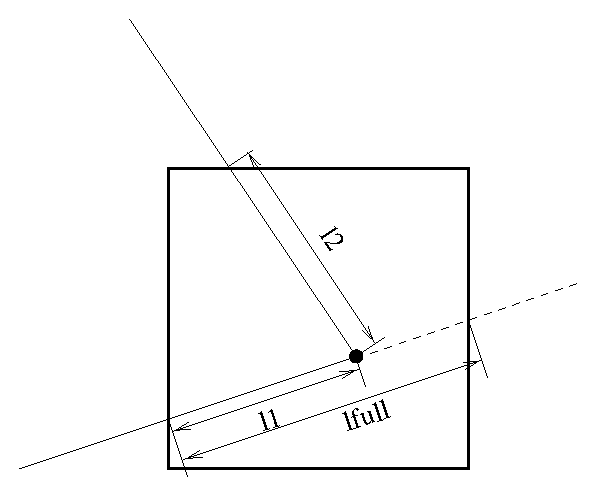
\includegraphics[width=0.6\textwidth]{figures/scatter.eps}
  \end{center}
\caption{The geometry of a scattering event within a powder sample.}
\label{powderFig}
\end{figure}

The probability for a neutron to be scattered from within the interval
$[ l_1 ; l_1+dl ]$ will be
\begin{equation}
\Pi(l_1) dl = \mu^s P(l_1) dl ,
\end{equation}
while the probability for a neutron to be scattered from within
this interval into the solid angle $\Omega$ {\em and}
not being scattered further
or absorbed on the way out of the sample is
\begin{equation}
\Pi(l_1,\Omega) dl d\Omega =
  \mu^s P(l_1) P(l_2) \gamma(\Omega) d\Omega dl ,
\end{equation}
where $\gamma(\Omega)$ is the directional distribution
of the scattered neutrons, and $l_2$ is determined by $l_1$,
$\Omega$, and the sample geometry, see figure \ref{powderFig}.

In our Monte-Carlo simulations, we will often choose the scattering
parameters by making a Monte-Carlo choice of $l_1$ and $\Omega$
from a distribution different from $\Pi(l_1,\Omega)$.
By doing this, we must adjust $\pi_i$ according to
the probability transformation rule (\ref{probrule}).
If we {\em e.g.}\ choose the scattering depth, $l_1$,
from a flat distribution in $[ 0 ; l_{\rm full} ]$,
and choose the directional dependence from $g(\Omega)$,
we have a Monte Carlo probability
\begin{equation}
f(l_1,\Omega) = g(\Omega) / l_{\rm full} ,
\end{equation}
$l_{\rm full}$ is here the path length through the sample
as taken by a non-scattered neutron (although we here
assume that all simulated neutrons are being scattered).
According to (\ref{probrule}), the neutron weight factor
is now adjusted by the amount
\begin{equation}     \label{sampleprob}
\pi_i(l_1,\Omega) =
 \mu^s l_{\rm full} \exp \left[ - (l_1+l_2) (\mu^a + \mu^s) \right]
  \frac{\gamma(\Omega)}{g(\Omega)} .
\end{equation}

In analogy with the source components, it is possible to define
interesting directions for the scattering.
One will then try to focus the scattered neutrons,
choosing a $g(\Omega)$, which peaks around these directions.
To do this, one uses (\ref{sampleprob}), where the
fraction $\gamma(\Omega)/g(\Omega)$ corrects for the focusing.
One must choose a proper distribution so that
$g(\Omega) > 0$ in every interesting direction. If this is not the
case, the Monte Carlo simulation gives incorrect results.

All samples of the powder type have been constructed with a focusing
and a non-focusing option.


\section{Powder1: A general powder sample}
\index{Samples!Powder, single diffraction line}
\index{Diffraction}
\subsection{General considerations}
An ideal powder sample consists of many small
crystallites, although each crystallite is sufficiently
large not to cause size broadening.
The orientation of the crystallites is evenly distributed,
and there is thus always a certain number of
crystallites oriented to fulfill the Bragg condition
\begin{equation}   \label{Bragg}
n \lambda = 2 d \sin \theta ,
\end{equation}
where $n$ is the order of the scattering (an integer), $\lambda$
is the neutron wavelength, $d$ is the lattice spacing of the sample,
and $2 \theta$ is the scattering angle, see figure \ref{coneFig}.
As all crystal orientations
are realised in a powder sample, the neutrons are scattered within a
{\em Debye-Scherrer cone} of opening angle $4 \theta$ \cite{bacon}.

\begin{figure}
  \begin{center}
    \psfrag{2theta}[c][c]{$2\theta$}
    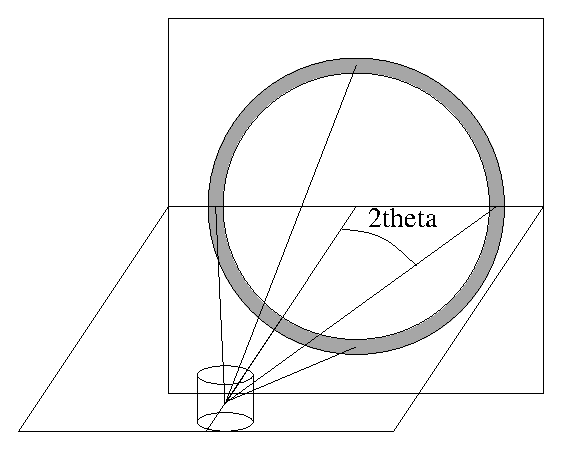
\includegraphics[width=0.6\textwidth]{figures/powder.eps}
  \end{center}
\caption{The scattering geometry of a powder sample showing the
Debye-Scherrer cone and the Debye-Scherrer circle.}
\label{coneFig}
\end{figure}

Equation (\ref{Bragg}) may be cast into the form
\begin{equation}
|{\bf Q}| = 2 |{\bf k}| \sin \theta ,
\end{equation}
where {\bf Q} is a vector of the reciprocal lattice, and {\bf k} is
the wave vector of the neutron. It is seen that only
reciprocal vectors fulfilling $|{\bf Q}| < 2 |{\bf k}|$
contribute to the scattering.
For a complete treatment of the powder sample, one needs to take
into account all these {\bf Q}-values, since each of them contribute
to the attenuation.

The textbook expression for the scattering intensity
from one reflection in a slab-shaped powder sample,
much larger than the beam cross section, reads \cite{bacon}
\begin{eqnarray}
\label{e:slab}
\frac{P}{P_0} &=& \frac{\lambda^3 l_s}{4\pi r} \frac{\rho'}{\rho}
         t j N_c^2 |F({\bf Q})|^2 \exp(-2W)
         \frac{\exp(-\mu^{\rm a} t / cos \theta)}{\sin^2(2\theta)} \\
|F({\bf Q})|^2 &=&
 \left| \sum_j b_j \exp({\bf R}_j \cdot {\bf Q}) \right|^2 ,
\end{eqnarray}
where the sum in the structure factor runs over all atoms in one unit cell.
The meanings and units of the symbols are
%
\begin{quote}\begin{tabular}{ccl}
$P_0$ & s$^{-1}$ & Incoming intensity of neutrons \\
$P$   & s$^{-1}$ & Detected intensity of neutrons \\
$l_s$ & m        & Height of detector \\
$r$   & m        & Distance from sample to detector \\
$\rho'/\rho$ & 1 & Packing factor of the powder \\
$t$   & m        & Slab thickness \\
$j$   & 1        & Multiplicity of the reflection \\
$N_c$ & m$^{-3}$ & Density of unit cells in bulk material\\
$|F({\bf Q})|^2$ & m$^2$  & Structure factor \\
$\exp(-2W)$ & 1  & Debye-Waller factor \\
$\mu^a$ & m$^{-1}$ & Linear attenuation factor due to absorption. \\
\end{tabular}\end{quote}
%
In analogy with this, the textbook expression for a cylinder shaped powder
sample, completely illuminated by the beam, reads \cite{bacon}
\begin{equation}
\frac{P}{\Psi_0} =
 \frac{V \rho'}{\rho} N_c^2 |F({\bf Q})|^2 j \exp(-2W)
                    \frac{A_{hkl}}{\sin(\theta)\sin(2\theta)}
                    \frac{l_s}{2\pi r} \frac{\lambda^3}{4} ,
\end{equation}
where the new symbols are
%
\begin{quote}\begin{tabular}{ccl}
$\Psi_0$  & s$^{-1}$m$^{-2}$ & Incoming beam flux \\
$V$       & m$^3$    & Sample volume \\
$A_{hkl}$ & 1        & Attenuation factor. \\
\end{tabular}\end{quote}
%
Eq.\ (\ref{e:slab}) for a slab shaped sample
may be cast into the form of the cylinder expression above
by using the substitutions
%
\begin{quote}\begin{tabular}{lrcl}
Incoming flux & $P_0 / (w h \cos\theta)$ & $\rightarrow$ & $\Psi_0$ \\
Sample volume & $w h t$ & $\rightarrow$ & $V$ \\
Absorption factor & $\exp(-\mu^a t / \cos\theta)$ & $\rightarrow$ & $A_{hkl}$, \\
\end{tabular}\end{quote}
%
where $h$ and $w$ are the height and width of the sample, respectively.
Often, one defines the {\em scattering power} as
\begin{equation}
Q \equiv N^2 \frac{|F({\bf Q})|^2 \lambda^3}{V \sin(2\theta)}
 = N_c^2 V \frac{\rho'}{\rho} \frac{|F({\bf Q})|^2 \lambda^3}{\sin(2\theta)} ,
\end{equation}
where $N$ is the number of unit cells.

A cut though the Debye-Scherrer cone perpendicular to its axis
is a circle. At the distance $r$ from the sample, the radius of this
circle is $r \sin(2\theta)$. Thus, the detector (in a small angle
approximation) only counts a fraction $f_d = l_s / (2 \pi r \sin(2 \theta))$
of the scattered neutrons.
One may now calculate the
linear attenuation coefficient in the material due to scattering
(from one {\bf Q}-value only):
\begin{equation}
\label{e:attenu}
\mu^s \equiv -\frac{1}{P_0} \frac{d(P/f_d)}{dl}
  = \frac{Q}{V} j \exp(-2W) \cos(\theta) .
\end{equation}
A powder sample will in general have several allowed reflections
${\bf Q}_j$, which will all contribute to the attenuation.
These reflections will have different values of
$|F({\bf Q}_j)|^2$ (and hence of $Q_j$), $j_j$, $\exp(-2W_j)$,
and $\theta_j$.
The total attenuation through the sample due to scattering is given by
$\mu^s = \mu_{\rm inc}^s + \sum_j \mu^s_j $,
where $\mu_{\rm inc}^s$ represents the incoherent scattering.

\subsection{This implementation}
For component {\bf Powder1}, we assume that the sample
has the shape of a solid cylinder.
Further, the incoherent scattering is only taken into account
by the attenuation of the beam, given by (\ref{e:attenu})
and $\sigma_c^a$.
The incoherently scattered neutrons are not
propagated through to the detector, but rather not generated at all.
Focusing is performed by only scattering into one angular
interval, $d\phi$ of the Debye-Scherrer circle. The center of this
interval is located at the point where the Debye-Scherrer circle
intersects the half-plane defined by the initial velocity, ${\bf v}_{\rm i}$,
and a user-specified vector, {\bf f}.
Multiple scattering is not implemented.

The input parameters for this component are
%
\begin{quote}\begin{tabular}{ccl}
$r$ & m & Radius of cylinder \\
$h$ & m & Height of cylinder \\
$\sigma_c^a$ & fm$^2$ & Absorption cross section per unit cell (at 2200 m/s) \\
$\sigma_{i,c}^s$ & (fm)$^2$ & Incoherent scattering cross section per unit cell \\
$\rho'/\rho$ & 1 & Packing factor \\
$V_c$ & \AA$^3$ & Volume of unit cell \\
${\bf Q}$ & \AA$^{-1}$ & The reciprocal lattice vector under consideration \\
$|F({\bf Q}_j)|^2$ & (fm)$^2$ &
 Structure factor \\
$j$ & 1 & Multiplicity of reflection \\
$\exp(-2W)$ & 1 & Debye-Waller factor \\
$d\phi$ & deg & Angular interval of focusing \\
$f_x$ & m & \\
$f_y$ & m & Focusing vector\\
$f_z$ & m & \\
\end{tabular}\end{quote}
%
The source text for the component is shown in Appendix
\ref{c:powder1}.

In a later version, more reciprocal lattice vectors will be
allowed.

          \newpage
\section{Single\_crystal: The single crystal component}
\label{s:Single_crystal}
\index{Samples!Single crystal diffraction}
\index{Diffraction}
\index{Incoherent elastic scattering}
\index{Multiple scattering}

\component{Single\_crystal}{Kristian Nielsen}{$x_{width}, y_{height}, z_{thick}$,$\vec a, \vec b, \vec c, \Delta d/d$, mosaic, reflections}{$\sigma_{abs}, \sigma_{inc}$, ...}{Partially validated, centered. Further validation undergoing. Known BUGS: The component is known not to work as a Bragg monochromator, likely the problem relates to the internal definition of the reciprocal space. Possibly related to this, the model of anistropic mosaic is broken - always use a non-zero isotropic mosaic. Also, always use a non-zero value of the $\Delta d/d$ parameter.}

The {\bf Single\_crystal} component models a thick, flat single crystal
with multiple scattering and absorption with elastic coherent scattering.
An elastic incoherent background may also be simulated.
It may be used to describe samples for diffraction,
but also for accurate monochromator descriptions.
The component is currently under further review. The current documentation is outdated, especially with respect to the model of crystal mosaicity.

The input parameters for the component are \textit{xwidth},
\textit{yheight}, and \textit{zthick} to define the dimensions of the
crystal in meters (area is centered); \textit{delta\_d\_d} to give the
value of $\Delta d/d$ (no unit);
$(\textit{ax}, \textit{ay}, \textit{az})$, $(\textit{bx}, \textit{by},
\textit{bz})$, and $(\textit{cx}, \textit{cy}, \textit{cz})$ to define
the axes of the direct lattice of the crystal (the sides of the unit
cell) in units of {\AA}ngstr{\o}m; and \textit{reflections}, a string
giving the name of the file with the list of structure factors to
consider.
The mosaic is specified \emph{either} isotropically as
\textit{mosaic}, \emph{or} anisotropically as \textit{mosaic\_h}
(rotation around the $Y$ axis), \textit{mosaic\_v} (rotation around the
$Z$ axis), and \textit{mosaic\_n} (rotation around the $X$ axis); in all
cases in units of full-width-half-maximum minutes of arc.

Optionally, the absorption cross-section at 2200 m/s and the incoherent
cross-section may be given as \textit{absorption} and
\textit{incoherent} (in barns), with default of zero; and
\textit{p\_transmit} may be assigned a fixed Monte Carlo probability for
transmission through the crystal without any interaction.

The user must specify a list of reciprocal lattice vectors
$\boldsymbol{\tau}$ to consider along with their structure factors
$|F_{\boldsymbol{\tau}}|^2$. The user must also specify the coordinates
(in direct space) of the unit cell axes $\boldsymbol{a}$,
$\boldsymbol{b}$, and $\boldsymbol{c}$, from which the reciprocal lattice
will be computed. See section \ref{s:Single_crystal_implement} for file format specifications.

In addition to coherent scattering, {\bf Single\_crystal} also
handles incoherent scattering and absorption. The incoherent scattering
cross-section is supplied by the user as a constant
$\sigma_{\rm inc}$. The absorption cross-section is supplied by the user at
2200~m/s, so the actual cross-section for a neutron of velocity $v$ is
$\sigma_{\rm abs} = \sigma_{2200} \frac{\rm 2200~m/s}{v}$.

\subsection{The physical model}

The textbook expression for the scattering cross-section of a crystal
is~\cite[ch.3]{squires}:
\begin{equation}
\label{eq:sigma_coh_el}
\left(\frac{d\sigma}{d\Omega}\right)_{\rm coh.el.} =
        N\frac{(2\pi)^3}{V_0}\sum_{\boldsymbol{\tau}}
        \delta(\boldsymbol{\tau} - \boldsymbol{\kappa})|F_{\boldsymbol{\tau}}|^2
\end{equation}
Here $|F_{\boldsymbol{\tau}}|^2$ is the structure factor
(defined in section~\ref{powder}), $N$ is the
number of unit cells, $V_0$ is the volume of an
individual unit cell, and $\boldsymbol{\kappa} (= {\bf k}_i - {\bf k}_f)$
is the scattering vector. $\delta(\boldsymbol{x})$ is a 3-dimensional delta
function in reciprocal space,
so for given incoming wave vector ${\bf k}_i$ and lattice vector
${\boldsymbol{\tau}}$, only a single final wave vector ${\bf k}_f$ is allowed.
In general, this wavevector will not fulfill the conditions for elastic
scattering $(k_f = k_i)$.
In a real crystal, however, reflections are not perfectly sharp. Because
of imperfection and finite-size effects, there will be a small region
around $\boldsymbol{\tau}$ in reciprocal space of possible scattering vectors.

{\bf Single\_crystal} simulates a crystal with a mosaic spread
$\eta$ and a lattice plane spacing uncertainty $\Delta d/d$. In such
crystals the reflections will not be completely sharp;
there will be a small region around each reciprocal lattice point of the
crystal that contains valid scattering vectors.

We model the mosaicity and $\Delta d/d$ of the crystal with
3-dimensional Gaussian functions in reciprocal space (see
figure~\ref{fig:crystal-reciprocal-space}). Two of the axes of the
Gaussian are perpendicular to the reciprocal lattice vector $\boldsymbol{\tau}$ and model
the mosaicity. The third one is parallel to $\boldsymbol{\tau}$ and models
$\Delta d/d$. We assume that the
mosaicity is small so that the possible directions of the scattering
vector may be approximated with a Gaussian in rectangular
coordinates.
\begin{figure}[t]
  \begin{center}
    \psfrag{ki}[r][r]{$\boldsymbol{k}_{\rm i}$}
    \psfrag{kf}[l][l]{$\boldsymbol{k}_{\rm f}$}
    \psfrag{tau}[r][r]{$\boldsymbol{\tau}$}
    \psfrag{mosaic}[l][l]{$\eta$}
    \psfrag{del-d-d}[l][l]{$\Delta d/d$}
    \psfrag{Ewald}[l][l]{Ewald}
    \psfrag{Sphere}[l][l]{Sphere}
    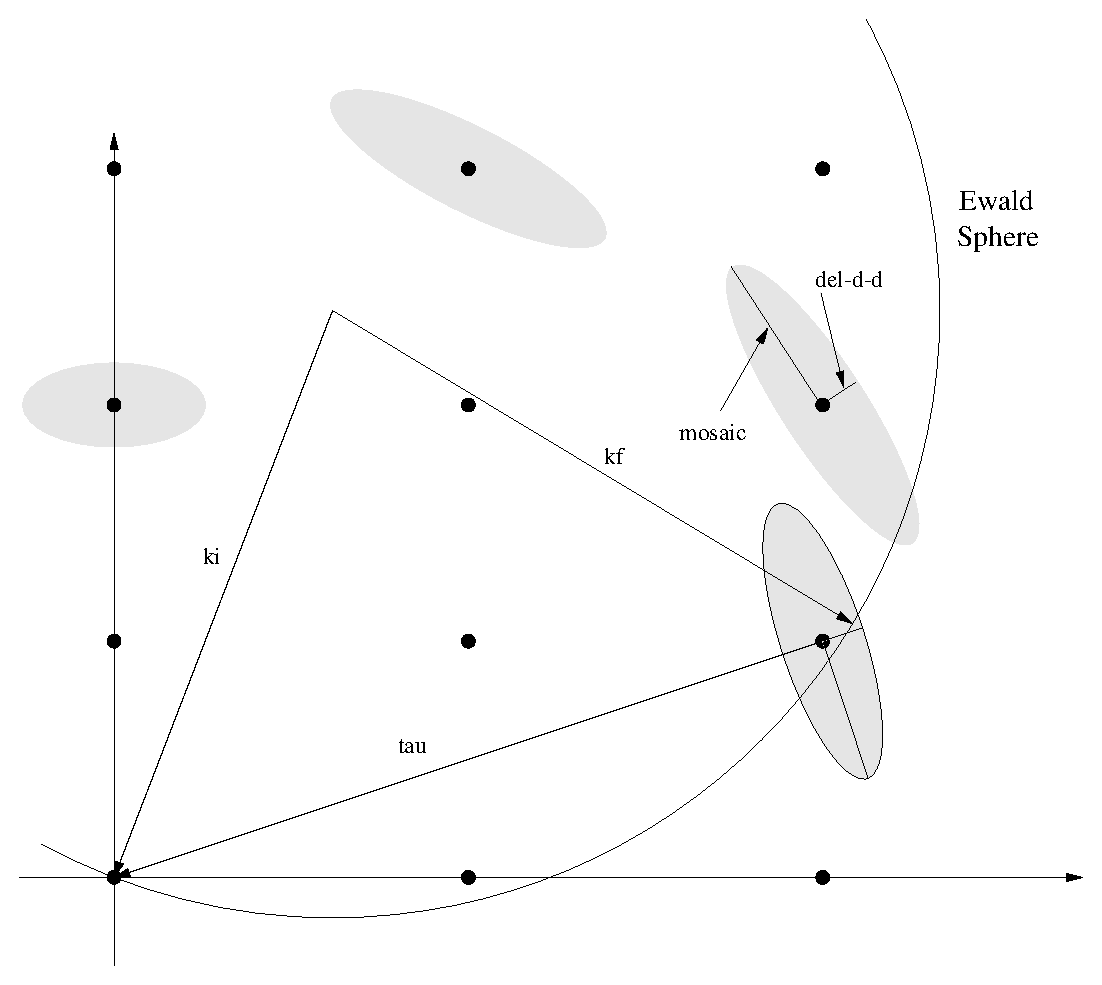
\includegraphics[width=0.7\textwidth]{figures/recip_space3.eps}
  \end{center}
\caption{Ewald sphere construction for a single neutron showing the
    Gaussian broadening of reciprocal lattice points in their local
    coordinate system.}
\label{fig:crystal-reciprocal-space}
\end{figure}

If the mosaic is isotropic (the same in all directions), the two
Gaussian axes perpendicular to $\boldsymbol{\tau}$ are simply arbitrary
normal vectors of equal length given by the mosaic. But if the mosaic
is anisotropic, the two perpendicular axes will in general be different
for each scattering vector. In the absence of anything better,
{\bf Single\_crystal} uses a model which is at least mathematically
plausible and which works as expected in the two common cases:
(1)~isotropic mosaic, and (2)~two mosaic directions (``horizontal and
vertical mosaic'') perpendicular to a scattering vector.

The basis for the model is a three-dimensional Gaussian distribution in
Euler angles giving the orientation probability distribution for the
micro-crystals; that is, the misorientation is given by small rotations
around the $X$, $Y$, and $Z$ axes, with the rotation angles having (in
general different) Gaussian probability distributions. For given
scattering vector $\boldsymbol{\tau}$, a rotation of the micro-crystals
around an axis parallel to $\boldsymbol{\tau}$ has no effect on the
direction of the scattering vector. Suppose we form the intersection
between the three-dimensional Gaussian in Euler angles and a plane
through the origin perpendicular to $\boldsymbol{\tau}$. This gives a
two-dimensional Gaussian, say with axes defined by unit vectors
$\boldsymbol{g}_1$ and $\boldsymbol{g}_2$ and mosaic widths $\eta_1$ and
$\eta_2$.

We now let the mosaic for $\boldsymbol{\tau}$ be defined by rotations
around $\boldsymbol{g}_1$ and $\boldsymbol{g}_2$ with angles having
Gaussian distributions of widths $\eta_1$ and $\eta_2$. Since
$\boldsymbol{g}_1$, $\boldsymbol{g}_2$, and $\boldsymbol{\tau}$ are
perpendicular, a small rotation of $\boldsymbol{\tau}$ around
$\boldsymbol{g}_1$ will change $\boldsymbol{\tau}$ in the direction of
$\boldsymbol{g}_2$. The two axes of the Gaussian mosaic in reciprocal
space that are perpendicular to $\boldsymbol{\tau}$ will thus be given
by $\tau\eta_2\boldsymbol{g}_1$ and $\tau\eta_1\boldsymbol{g}_2$.

We now derive a quantitative expression for the scattering cross-section
of the crystal in the model. For this, we introduce a \emph{local
  coordinate system} for each reciprocal lattice point
$\boldsymbol{\tau}$ and use $\boldsymbol{x}$ for vectors written in local
coordinates. The origin is $\boldsymbol{\tau}$, the first axis
is parallel to $\boldsymbol{\tau}$ and the other two axes are
perpendicular to $\boldsymbol{\tau}$. In the local coordinate system,
the 3-dimensional Gaussian is given by
\begin{equation}
  \label{eq:crystal-gauss-1}
  G(x_1,x_2,x_3) = \frac{1}{(\sqrt{2\pi})^3}\frac{1}{\sigma_1\sigma_2\sigma_3}
  e^{-\frac{1}{2}(\frac{x_1^2}{\sigma_1^2} +
  \frac{x_2^2}{\sigma_2^2} + \frac{x_3^2}{\sigma_3^2})}
\end{equation}
The axes of the Gaussian are $\sigma_1 = \tau\Delta d/d$ and $\sigma_2 =
\sigma_3 = \eta\tau$. Here we used the assumption that $\eta$ is small,
so that $\tan\eta \approx \eta$ (with $\eta$ given in radians).  By
introducing the diagonal matrix
$$
D = \left(
  \begin{array}[c]{ccc}
    \frac{1}{2}\sigma_1^2 & 0 & 0 \\
    0 & \frac{1}{2}\sigma_2^2 & 0 \\
    0 & 0 & \frac{1}{2}\sigma_3^2
  \end{array}\right)
$$
equation~(\ref{eq:crystal-gauss-1}) can be written as
\begin{equation}
  G(\boldsymbol{x}) =
  \frac{1}{(\sqrt{2\pi})^3}\frac{1}{\sigma_1\sigma_2\sigma_3}
  e^{-\boldsymbol{x}^{\rm T} D \boldsymbol{x}}
\end{equation}
again with $\boldsymbol{x}=(x_1,x_2,x_3)$ written in local coordinates.

To get an expression in the coordinates of the reciprocal lattice of the
crystal, we introduce a matrix $U$ such that if $\boldsymbol{y} =
(y_1,y_2,y_3)$ are the global coordinates of a point in the crystal
reciprocal lattice, then $U(\boldsymbol{y} + \boldsymbol{\tau})$ are the
coordinates in the local coordinate system for $\boldsymbol{\tau}$. The
matrix $U$ is given by
$$ U^{\rm T} = (\hat{u}_1, \hat{u}_2, \hat{u}_3), $$
where $\hat{u}_1$, $\hat{u}_2$, and $\hat{u}_3$ are the axes of the
local coordinate system, written in the global coordinates of the
reciprocal lattice. Thus
$\hat{u}_1 = \boldsymbol{\tau}/\tau$,  and $\hat{u}_2$ and $\hat{u}_3$ are
unit vectors perpendicular to $\hat{u}_1$ and to each other.
The matrix $U$ is unitarian, that is
$U^{-1} = U^{\rm T}$. The translation between global and local
coordinates is
$$ \boldsymbol{x} = U(\boldsymbol{y} + \boldsymbol{\tau}) \qquad
   \boldsymbol{y} = U^{\rm T} \boldsymbol{x} - \boldsymbol{\tau} $$

The expression for the 3-dimensional Gaussian in global coordinates is
\begin{equation}
  G(\boldsymbol{y}) =
  \frac{1}{(\sqrt{2\pi})^3}\frac{1}{\sigma_1\sigma_2\sigma_3}
  e^{-(U(\boldsymbol{y}+\boldsymbol{\tau}))^{\rm T} D (U(\boldsymbol{y}+\boldsymbol{\tau}))}
\end{equation}
The elastic coherent cross-section is then given by
\begin{equation}
  \label{eq:crystal-cross-section}
  \left(\frac{d\sigma}{d\Omega}\right)_{\rm coh.el.} =
        N\frac{(2\pi)^3}{V_0}\sum_{\boldsymbol{\tau}}
        G(\boldsymbol{\tau} - \boldsymbol{\kappa})
         |F_{\boldsymbol{\tau}}|^2
\end{equation}

\subsection{The algorithm}

The overview of the algorithm used in the Single\_crystal component is
as follows:
\begin{enumerate}
\item\label{enum:crystal-1} Check if the neutron intersects the
  crystal. If not, no action is taken.
\item\label{enum:crystal-2} Search through a list of reciprocal lattice
  points of interest, selecting those that are close enough to the Ewald
  sphere to have a non-vanishing scattering probability. From these,
  compute the total coherent cross-section $\sigma_{\rm coh}$ (see
  below), the absorption cross-section $\sigma_{\rm abs} = \sigma_{\rm
  2200} \frac{{\rm 2200~m/s}}{v}$, and the total cross-section
  $\sigma_{\rm tot} = \sigma_{\rm coh}+\sigma_{\rm inc}+\sigma_{\rm abs}$.
\item\label{enum:crystal-3} The transmission probability is
  $\exp(- \frac{\sigma_{\rm tot}}{V_0}\ell)$ where $\ell$ is the length of
  the flight path through the crystal. A Monte Carlo choice is
  performed to determine
  whether the neutron is transmitted. Optionally, the user may
  set a fixed Monte Carlo probability for the first scattering event,
  for example to boost the statistics for a weak reflection.
\item\label{enum:crystal-4} For non-transmission, the position at which
  the neutron will interact is selected from an exponential
  distribution. A Monte Carlo choice is made of whether to scatter
  coherently or incoherently. Absorption is treated by weight adjustment
  (see below).
\item\label{enum:crystal-5} For incoherent scattering, the outgoing wave
  vector $\boldsymbol{k}_{\rm f}$ is selected with a random direction.
\item\label{enum:crystal-6} For coherent scattering, a reciprocal
  lattice vector is selected by a Monte Carlo choice, and
  $\boldsymbol{k}_{\rm f}$ is found (see below).
\item\label{enum:crystal-7} Adjust the neutron weight as dictated by the
  Monte Carlo choices made.
\item\label{enum:crystal-8} Repeat from~(\ref{enum:crystal-2}) until the
  neutron is transmitted (to simulate multiple scattering).
\end{enumerate}

For point~\ref{enum:crystal-2}, the distance
\textit{dist} between a reciprocal lattice point and the Ewald sphere is
considered small enough to allow scattering if it is less than five
times the maximum axis of the Gaussian, $\textit{dist} \leq
5\max(\sigma_1,\sigma_2,\sigma_3)$.

\subsection{Choosing the outgoing wave vector}

The final wave vector $\boldsymbol{k}_{\rm f}$ must lie on the
intersection between the Ewald sphere and the Gaussian ellipsoid. Since
$\eta$ and $\Delta d/d$ are assumed small, the intersection can be
approximated with a plane tangential to the sphere, see
figure~\ref{fig:crystal-scattering-tri}. The tangential point is taken
to lie on the line between the center of the Ewald sphere
$-\boldsymbol{k}_{\rm i}$ and the reciprocal lattice point
$\boldsymbol{\tau}$. Since the radius of the Ewald sphere is $k_{\rm
  i}$, this point is
$$ \boldsymbol{o}=(k_{\rm i}/\rho - 1)\boldsymbol{\rho} - \boldsymbol{\tau} $$
where $\boldsymbol{\rho} = \boldsymbol{k}_{\rm i} - \boldsymbol{\tau}$.
\begin{figure}[t]
  \begin{center}
    \psfrag{ki}[r][r]{$\boldsymbol{k}_{\rm i}$}
    \psfrag{kf}[l][l]{$\boldsymbol{k}_{\rm f}$}
    \psfrag{rho}[r][r]{$\boldsymbol{\rho}$}
    \psfrag{tau}[r][r]{$\boldsymbol{\tau}$}
    \psfrag{x}[l][l]{$\boldsymbol{x}$}
    \psfrag{Ewald}[r][r]{Ewald}
    \psfrag{Sphere}[r][r]{Sphere}
    \psfrag{Tangential}[l][l]{Tangential}
    \psfrag{plane}[l][l]{plane}
    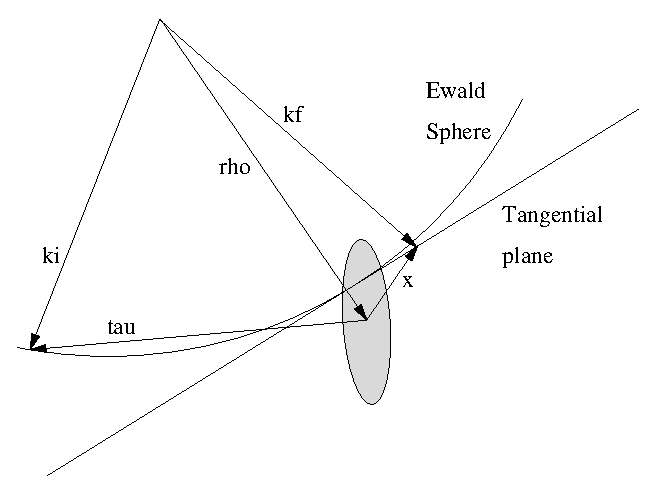
\includegraphics[width=0.7\textwidth]{figures/recip-detail.eps}
  \end{center}
\caption{The scattering triangle in the single crystal.}
\label{fig:crystal-scattering-tri}
\end{figure}

The equation for the plane is
\begin{equation}
  \label{eq:crystal-tangent-plane}
    \boldsymbol{P}(\boldsymbol{t}) = \boldsymbol{o} + B \boldsymbol{t}, \qquad
    \boldsymbol{t} \in \mathbb{R}^2
\end{equation}
Here $B = (\boldsymbol{b}_1, \boldsymbol{b}_2)$ is a $3\times 2$ matrix
with the two generators for the plane $\boldsymbol{b}_1$ and
$\boldsymbol{b}_2$. These are (arbitrary) unit vectors in the plane,
being perpendicular to
each other and to the plane normal $\boldsymbol{n} =
\boldsymbol{\rho}/\rho$.

Each $\boldsymbol{t}$ defines a potential final wave vector
$\boldsymbol{k}_{\rm f}(\boldsymbol{t}) = \boldsymbol{k}_{\rm i} +
\boldsymbol{P}(\boldsymbol{t})$. The value of the 3-dimensional Gaussian
for this $\boldsymbol{k}_{\rm f}$ is
\begin{equation}
  \label{eq:crystal-gauss-t-1}
  G(\boldsymbol{x}(\boldsymbol{t})) =
  \frac{1}{(\sqrt{2\pi})^3}\frac{1}{\sigma_1\sigma_2\sigma_3}
  e^{-\boldsymbol{x}(\boldsymbol{t})^{\rm T} D \boldsymbol{x}(\boldsymbol{t})}
\end{equation}
where $\boldsymbol{x}(\boldsymbol{t}) = \boldsymbol{\tau} -
(\boldsymbol{k}_{\rm i} - \boldsymbol{k}_{\rm f}(\boldsymbol{t}))$ is
given in local coordinates for $\boldsymbol{\tau}$. It can be shown that
equation~(\ref{eq:crystal-gauss-t-1}) can be re-written as
\begin{equation}
  \label{eq:crystal-gauss-2}
  G(\boldsymbol{x}(\boldsymbol{t})) =
  \frac{1}{(\sqrt{2\pi})^3}\frac{1}{\sigma_1\sigma_2\sigma_3} e^{-\alpha}
  e^{-(\boldsymbol{t}-\boldsymbol{t}_0)^{\rm T} M
    (\boldsymbol{t}-\boldsymbol{t}_0)}
\end{equation}
where $M = B^{\rm T} D B$ is a $2 \times 2$ symmetric and positive
definite matrix, $\boldsymbol{t}_0 = -M^{-1}B^{\rm T} D \boldsymbol{o}$
is a 2-vector, and $\alpha = -\boldsymbol{t}_0^{\rm T} M
\boldsymbol{t}_0 + \boldsymbol{o}^{\rm T} D \boldsymbol{o}$ is a real
number.  Note that this is a two-dimensional Gaussian (not necessarily
normalized) in $\boldsymbol{t}$ with center $\boldsymbol{t}_0$ and axis
defined by $M$.

To choose $\boldsymbol{k}_{\rm f}$ we sample $\boldsymbol{t}$ from the
2-dimensional Gaussian distribution~(\ref{eq:crystal-gauss-2}). To do
this, we first construct the Cholesky decomposition of the matrix
$(\frac{1}{2}M^{-1})$. This gives a $2\times 2$ matrix $L$ such that $L
L^{\rm T} = \frac{1}{2}M^{-1}$ and is possible since $M$ is symmetric
and positive definite. It is given by
$$
  L = \left(
  \begin{array}[c]{cc}
    \sqrt{\nu_{11}} & 0 \\
    \frac{\nu_{12}}{\sqrt{\nu_{11}}} & \sqrt{\nu_{22} - \frac{\nu_{12}^2}{\nu_{11}}}
  \end{array}\right)
\qquad\hbox{where }
  \frac{1}{2}M^{-1} = \left(
  \begin{array}[c]{cc}
    \nu_{11} & \nu_{12} \\
    \nu_{12} & \nu_{22}
  \end{array}\right)
$$
Now let $\boldsymbol{g} = (g_1, g_2)$ be two random numbers drawn form a
Gaussian distribution with mean 0 and standard deviation 1, and let
$\boldsymbol{t} = L\boldsymbol{g} + \boldsymbol{t}_0$. The probability
of a particular $\boldsymbol{t}$ is then
\begin{eqnarray}
  P(\boldsymbol{t})d\boldsymbol{t}
    &=& \frac{1}{2\pi}
      e^{-\frac{1}{2}\boldsymbol{g}^{\rm T}\boldsymbol{g}} d\boldsymbol{g} \\
    &=& \frac{1}{2\pi}\frac{1}{\det L}
      e^{-\frac{1}{2}(L^{-1}(\boldsymbol{t}-\boldsymbol{t}_0))^{\rm T}
          (L^{-1}(\boldsymbol{t}-\boldsymbol{t}_0))} d\boldsymbol{t} \\
    &=& \frac{1}{2\pi}\frac{1}{\det L}
      e^{-(\boldsymbol{t}-\boldsymbol{t}_0)^{\rm T}
          M(\boldsymbol{t}-\boldsymbol{t}_0)} d\boldsymbol{t}
  \label{eq:crystal-gauss-prob-1}
\end{eqnarray}
where we used that
$\boldsymbol{g}=L^{-1}(\boldsymbol{t}-\boldsymbol{t}_0)$ so that
$d\boldsymbol{g} = \frac{1}{\det L}d\boldsymbol{t}$. This is just the
normalized form of~(\ref{eq:crystal-gauss-2}). Finally we set
$\boldsymbol{k}'_{\rm f} = \boldsymbol{k}_{\rm i} +
\boldsymbol{P}(\boldsymbol{t})$ and
$\boldsymbol{k}_{\rm f} = (k_{\rm i}/k'_f)\boldsymbol{k}'_{\rm f}$ to
normalize the length of $\boldsymbol{k}_{\rm f}$ to correct for the
(small) error introduced by approximating the Ewald sphere with a plane.

\subsection{Computing the total coherent cross-section}

To determine the total coherent scattering cross-section, the differential
cross-section must be integrated over the Ewald sphere:
$$
\sigma_{\rm coh} = \int_{\rm Ewald}
\left(\frac{d\sigma}{d\Omega}\right)_{\rm coh.el.} d\Omega
$$
For small mosaic we may approximate the sphere with the tangential
plane, and we thus get from~(\ref{eq:crystal-cross-section})
and~(\ref{eq:crystal-gauss-2}):
\begin{eqnarray}
  \label{eq:crystal-coh-cs}
  \sigma_{{\rm coh},\boldsymbol{\tau}} &=& \int N\frac{(2\pi)^3}{V_0}
        G(\boldsymbol{\tau} - \boldsymbol{\kappa})
         |F_{\boldsymbol{\tau}}|^2 d\Omega \\
  &=& \frac{1}{\boldsymbol{k}_i^2} N\frac{(2\pi)^3}{V_0}
         \frac{1}{(\sqrt{2\pi})^3}\frac{e^{-\alpha}}{\sigma_1\sigma_2\sigma_3}
         |F_{\boldsymbol{\tau}}|^2
         \int e^{-(\boldsymbol{t}-\boldsymbol{t}_0)^{\rm T} M
         (\boldsymbol{t}-\boldsymbol{t}_0)}
         d\boldsymbol{t} \\
  &=& \det(L) \frac{1}{\boldsymbol{k}_i^2} N\frac{(2\pi)^{3/2}}{V_0}
         \frac{e^{-\alpha}}{\sigma_1\sigma_2\sigma_3}
         |F_{\boldsymbol{\tau}}|^2
         \int e^{-\frac{1}{2}\boldsymbol{g}^{\rm T}\boldsymbol{g}}
         d\boldsymbol{g} \\
  &=& 2\pi\det(L) \frac{1}{\boldsymbol{k}_i^2} N\frac{(2\pi)^{3/2}}{V_0}
         \frac{e^{-\alpha}}{\sigma_1\sigma_2\sigma_3}
         |F_{\boldsymbol{\tau}}|^2 \\
  &=& \frac{\det(L)}{\boldsymbol{k}_i^2} N\frac{(2\pi)^{5/2}}{V_0}
         \frac{e^{-\alpha}}{\sigma_1\sigma_2\sigma_3}
         |F_{\boldsymbol{\tau}}|^2 \\
  \sigma_{\rm coh} &=& \sum_{\boldsymbol{\tau}} \sigma_{{\rm coh},\boldsymbol{\tau}}
\end{eqnarray}
As before, we let $\boldsymbol{g} = L^{-1}(\boldsymbol{t} -
\boldsymbol{t}_0)$ so that $d\boldsymbol{t} = \det(L) d\boldsymbol{g}$.

\paragraph{Neutron weight factor adjustment}

We now calculate the correct neutron weight adjustment for the Monte
Carlo choices made. In three cases is a Monte Carlo choice made with a
probability different from the probability of the corresponding physical
event: When deciding whether to transmit the neutron or not, when
simulating absorption, and when selecting the reciprocal lattice vector
$\boldsymbol{\tau}$ to scatter from.

If the user has choosen a fixed transmission probability $f({\rm
  transmit}) = p_{\rm transmit}$, the neutron weight must be adjusted by
$$ \pi({\rm transmit}) = \frac{P({\rm transmit})}{f({\rm transmit})}
$$
where $P({\rm transmit}) = \exp(-\frac{\sigma_{\rm tot}}{V_0}\ell)$ is
the physical transmission probability. Likewise, for non-transmission
the adjustment is
$$ \pi({\rm no~transmission}) = \frac{1-P({\rm transmit})}{1-f({\rm transmit})}.
$$

Absorption is never explicitly simulated, so the Monte Carlo probability
of coherent or incoherent scattering is
$f({\rm coh})+f({\rm inc}) = 1$.
The physical probability of coherent or incoherent scattering is
$$ P({\rm coh})+P({\rm inc}) = \frac{\sigma_{\rm coh} + \sigma_{\rm
    inc}}{\sigma_{\rm tot}}, $$
so again a weight adjustment $\pi({\rm coh}|{\rm inc}) = \Pi({\rm
    coh}|{\rm inc})/f({\rm coh}|{\rm inc})$ is needed.

When choosing the reciprocal lattice vector $\boldsymbol{\tau}$ to
scatter from, the relative probability for $\boldsymbol{\tau}$ is
$r_{\boldsymbol{\tau}} = \sigma_{{\rm
    coh},\boldsymbol{\tau}}/|F_{\boldsymbol{\tau}}|^2$. This is done to
get better statistics for weak reflections. The Monte Carlo probability
for the reciprocal lattice vector $\boldsymbol{\tau}$ is thus
$$ f(\boldsymbol{\tau}) =
\frac{r_{\boldsymbol{\tau}}}{\sum_{\boldsymbol{\tau}} r_{\boldsymbol{\tau}}}
$$
whereas the physical probability is $P(\boldsymbol{\tau}) = \sigma_{{\rm
    coh},\boldsymbol{\tau}}/\sigma_{\rm coh}$. A weight adjustment is
thus needed of
$$
\pi(\boldsymbol{\tau}) =
 \frac{P(\boldsymbol{\tau})}{f(\boldsymbol{\tau})} =
 \frac{\sigma_{{\rm coh},\boldsymbol{\tau}}
  \sum_{\boldsymbol{\tau}} r_{\boldsymbol{\tau}}}
 {\sigma_{\rm coh} \; r_{\boldsymbol{\tau}}}.$$

In most cases, however, only one reflection is possible, whence $\pi=1$.

\subsection{Implementation details}
\label{s:Single_crystal_implement}

The equations describing {\bf Single\_crystal} are quite
complex, and consequently the code is fairly sizeable. Most of it is
just the expansion of the vector and matrix equations in individual
coordinates, and should thus be straightforward to follow.

The implementation pre-computes a lot of the necessary values in the
\texttt{INITIALIZE} section. It is thus actually very efficient despite
the complexity. If the list of reciprocal lattice points is big,
however, the search through the list will be slow. The precomputed data
is stored in the structures \texttt{hkl\_info} and in an array of
\texttt{hkl\_data} structures (one for each reciprocal lattice point in
the list). In addition, for every neutron event an array of
\texttt{tau\_data} is computed with one element for each reciprocal
lattice point close to the Ewald sphere. Except for the search for
possible $\boldsymbol{\tau}$ vectors, all computations are done in local
coordinates using the matrix $U$ to do the necessary transformations.

The list of reciprocal lattice points is specified in an ASCII data
file. Each line contains seven numbers, separated by white space. The
first three numbers are the $(h,k,l)$ indices of the reciprocal lattice
point, and the last number is the value of the structure factor
$|F_{\boldsymbol{\tau}}|^2$, in barns. The middle three numbers are not
used and may be omitted; they are nevertheless recommended since this makes
the file format compatible with the output from the Crystallographica
program~\cite{crystallographica}.
Any line beginning with any character of \verb+#;/%+ is considered to be a
comment, and lines which can not be read as vectors/matrices are ignored.

The column signification may also explicitely be set in the data file header using any of the lines:
\begin{verbatim}
  #column_h <index of the Bragg Qh column>
  #column_k <index of the Bragg Qk column>
  #column_l <index of the Bragg Ql column>
  #column_F2 <index of the squared str. factor '|F|^2' column [b]>
  #column_F  <index of the structure factor norm '|F|' column>
\end{verbatim}

Other component parameters may as well be specified in the data file
header with lines e.g.:
\begin{verbatim}
  #sigma_abs <value of Absorption cross section [barns]>
  #sigma_inc <value of Incoherent cross section [barns]>
  #Delta_d/d <value of Detla_d/d width for all lines>
  #lattice_a <value of the a lattice parameter [Angs]>
  #lattice_a <value of the b lattice parameter [Angs]>
  #lattice_a <value of the c lattice parameter [Angs]>
  #lattice_aa <value of the alpha lattice angle [deg]>
  #lattice_bb <value of the beta  lattice angle [deg]>
  #lattice_cc <value of the gamma lattice angle [deg]>
\end{verbatim}

Example data \verb+*.lau+ files are given in directory \verb+MCSTAS/data+.

These files contain an extensive self-documented header defining most the sample parameters, so that only the file name and mosaicity should be given to the component:
\begin{verbatim}
  Single_crystal(xwidth=0.01, yheight=0.01, zthick=0.01,
    mosaic = 5, reflections="YBaCuO.lau")
\end{verbatim}

Powder files from ICSD/LAZY \cite{icsd_ill} and Fullprof \cite{Fullprof}
may also be used (see Table \ref{t:powders-data}, page \pageref{t:powders-data}).
We do not recommend to use these as the equivalent $\vec q$ vectors are superposed, not
all Bragg spots will be simulated, and the intensity will not be scaled by the
multiplicity for each spot.

   \newpage
\section{Sans\_spheres: A sample of hard spheres for small-angle scattering}
\label{sans}
\index{Samples!Dilute colloid medium}
\index{Diffraction}
\index{Small angle scattering}

\component{Sans\_spheres}{(System); Lise Arleth, Veterinary University of Denmark}{$R$, $x_w$, $y_h$, $z_t$, $r$, $\sigma_a$, $\phi$, $\Delta \rho$, $R_{\rm det}$, $d$}{}{}

The component {\bf Sans\_spheres} models a sample of small independent
spheres of radius $R$, which are uniformly distributed
in a rectangular volume $x_w \times y_h \times z_t$ with a volume
fraction $\phi$. The absorption cross section density for the spheres
(or is it from the solution?)
is $\sigma_a$ (in units of m$^{-1}$), specified
for neutrons at 2200 m/s. Absorption and incoherent scattering 
from the medium is neglected.
The difference in scattering length density
(the contrast) between the hard spheres and the medium is called $\Delta \rho$.
$d$ denotes the distance to the (presumed circular) SANS detector of radius $R$.

\subsection{Small-angle scattering cross section}
The neutron intensity scattered into a solid angle $\Delta \Omega$
for a flat isotropic SANS sample in transmission geometry 
is given by \cite{ILLblue}:
\begin{equation}
I_s(q) = \Psi \Delta\Omega T A z_{\rm max} \frac{d\sigma_v}{d\Omega}(q) ,
\end{equation}
where $\Psi$ is the neutron flux, $T$ is the sample transmission,
$A$ is the illuminated sample area, and $z_{\rm max}$ the length of
the neutron path through the sample.

In this component, we consider only scattering from a thin solution
of monodisperse hard spheres of radius $R$, where the volume-specific
scattering cross section is given by \cite{ILLblue}
\begin{equation}
\frac{d\sigma_v}{d\Omega}(q) =
  n (\Delta\rho)^2 V^2 f(q)  ,
\end{equation}
where $f(q) = \left( 3\frac{\sin(qR)-qR\cos(qR)}{(qR)^3} \right)^2$,
$n$ is the number density of spheres, and $V = 4 / 3 \pi R^3$ is the
sphere volume. (The density is thus $n = \phi/V$.)

Multiple scattering is ignored.

\subsection{Algorithm}
All neutrons, which hit the sample volume, are scattered.
(Hence, no direct beam is simulated.)
For scattered neutrons, the following steps are taken:
\begin{enumerate}
\item Choose a value of $q$ uniformly in the interval $[0;q_{\rm max}]$.
\item Choose a polar angle, $\alpha$,
  for the {\bf q}-vector uniformly in $[0;\pi]$.
\item Scatter the neutron according to $(q,\alpha)$.
\item Calculate and apply the correct weight factor correction.
\end{enumerate}

\subsection{Calculating the weight factor}
The scattering position is found by a Monte Carlo choice uniformly
along the whole (unscattered) beam path with the sample, length $l_{\rm full}$, giving 
$f_l = 1/l_{\rm full}$. The direction focusing on the detector gives
(in an small angle approximation) $f_\Omega = d^2 / (\pi R_{\rm det}^2)$.

Hence, the total weight tranformation factor becomes (more explanation to come)
\begin{equation}
\pi_j = l_{\rm full} (\pi R_{\rm det}^2 / d^2)/(4 \pi)
  n (\Delta\rho)^2 V^2 f(q) \exp(-\mu_a l) , 
\end{equation}
where $\mu_a$ is the linear attenuation factor due to absorption
and $l$ is the total neutron path length within the sample.
              \newpage
\section{Phonon\_simple: A simple phonon sample}
\label{s:phonon_simple}
\index{Samples!Phonon scattering}
\index{Inelastic scattering}

\component{Phonon\_simple}{Kim Lefmann, Ris\o\ National Laboratory}{ $r_{\rm o}$, $h$, $r_{\rm foc}$, $x_{\rm target}$, $y_{\rm target}$, $z_{\rm target}$, $\sigma_{\rm abs}$, $\sigma_{\rm inc}$, $a$, $b$, $c$, $M$, $DW$, $T$}{$w_x$, $h_y$, $t_z$, $w_{\rm focus}, h_{\rm focus}$, $w_{\rm foc, angle}$, $h_{\rm foc, angle}$, target\_index}{only validated qualitatively}

This component models a simple phonon signal from a single crystal of
a pure element in an {\em fcc} crystal structure.
Only one isotropic acoustic phonon branch is modelled, and the longitudinal
and transverse dispersions are identical with the velocity of sound being $c$.
Other physical parameters are the atomic mass, $M$, the lattice parameter, $a$,
the scattering length, $b$,
the Debye-Waller factor, \verb+DW+, and the temperature, $T$.
Incoherent scattering and absorption are taken into account by the cross
sections $\sigma_{\rm abs}$ and $\sigma_{\rm inc}$.

The sample can have the form of a cylinder with height $h$ and radius
$r_0$, or a box with dimensions $w_x, h_y, t_z$.

Phonons are emitted into a specific range of solid angles, specified
by the location $(x_t, y_t, z_t)$ and the focusing radius, $r_0$.
Alternatively, the focusing is given by a rectangle,
$w_{\rm focus}$ and $h_{\rm focus}$, and the focus point is given by the
index of a down-stream component, \verb+target_index+.

Multiple scattering is not included in this component.

A usage example of this component can be found in the \verb+Neutron site/tests/Test_Phonon+ instrument from the \verb+mcgui+.

\subsection{The phonon cross section} % This is modified from the paper version %
The inelastic phonon cross section for a Bravais crystal of a pure element
is given by Ref.~\cite[ch.3~]{squires}
\begin{eqnarray}
\frac{d^2\sigma'}{d\Omega dE_{\rm f}} &=&
  b^2 \frac{k_{\rm f}}{k_{\rm i}} \frac{(2\pi)^3}{V_0}\frac{1}{2M} \exp(-2W) \nonumber \\
&\times&
  \sum_{\tau,q,p} \frac{(\mbox{\boldmath $\kappa$} \cdot {\bf e}_{q,p})^2}
                       {\omega_{q,p}}
  \left\langle n_{q,p} + \frac{1}{2} \mp \frac{1}{2} \right\rangle
  \delta(\omega\pm\omega_{q,p}) \delta(\kappa\pm{\bf q}-\tau) ,
\end{eqnarray}
where both annihilation and creation of one phonon is considered
(represented by the plus and minus sign in the dispersion delta functions,
respectively).
In the equation,
$\exp(-2W)$ is the Debye-Waller factor, \verb+DW+ and
$V_0 $ is the volume of the unit cell.
The sum runs over the reciprocal lattice vectors, $\tau$,
over the polarisation index, $p$,
and the $N$ allowed wave vectors {\bf q} within the Brillouin zone
(where $N$ is the number of unit cells in the crystal).
Further, ${\bf e}_{q,p}$ is the
polarization unit vectors, $\omega_{q,p}$ the phonon dispersion,
and the Bose factor is
$\langle n_{q,p} \rangle = (\hbar \exp(|\omega_{q,p}|/k_{\rm B}T)-1)^{-1}$.

We have simplified this expression by assuming no polarization
dependence of the dispersion, giving
$\sum_{p} (\mbox{\boldmath $\kappa$} \cdot {\bf e}_{q,p})^2 = \kappa^2$.
We assume that the inter-atomic interaction is nearest-neighbour-only
so that the phonon dispersion becomes:
\begin{equation}
d_1({\bf q}) = c_1/a \sqrt{z-s_q} ,
\end{equation}
where $z=12$ is the number of nearest neighbours and
$s_q=\sum_{\rm nn} \cos({\bf q} \cdot {\bf r}_{\rm nn})$,
where in turn ${\bf r}_{\rm nn}$ is the lattice positions of the
nearest neighbours.

This dispersion relation may be modified with a small effort,
since it is given as a separate c-function attatched to the component.

To calculate $d\sigma/d\Omega$ we need to transform the
{\bf q} sum into an integral over the Brillouin zone by
$\sum_q \rightarrow N V_{\rm c} (2\pi)^{-3} \int_{\rm BZ} d^3{\bf q}$.
The $\mbox{\boldmath $\kappa$}$ sum can now be removed by
expanding the {\bf q} integral to infinity.
All in all, the partial differential cross section reads
\begin{eqnarray}
\frac{d^2\sigma'}{d\Omega dE_{\rm f}}
  (\mbox{\boldmath $\kappa$},\omega) &=&
  N b^2 \frac{k_{\rm f}}{k_{\rm i}} \frac{1}{2M}
  \int \frac{\hbar \kappa^2}{\hbar \omega_q}
  \left\langle n_{q}+\frac{1}{2}\mp\frac{1}{2} \right\rangle
  \delta(\omega\pm\omega_{q}) \delta(\mbox{\boldmath $\kappa$}\pm{\bf q})
   d^3{\bf q} \nonumber \\
 &=& N b^2 \frac{k_{\rm f}}{k_{\rm i}}
          \frac{\hbar^2 \kappa^2}{2M \hbar \omega_q}
  \left\langle n_{\kappa}+\frac12\pm\frac12 \right\rangle
  \delta(\hbar\omega\pm d_1(\kappa)) . \label{e:phonon-pdcross}
\end{eqnarray}

\subsection{The algorithm}
All neutrons, which hit the sample volume, are scattered
into a particular range of solid angle, $\Delta \Omega$,
like many other components. One of the difficult things in
scattering from a dispersion is to take care to fulfill the
dispersion criteria and to find the correct weight transformation.

In {\bf Phonon\_simple}, the following steps are taken:
\begin{enumerate}
\item If the sample is hit, calculate the total path length inside the
sample, otherwise leave the neutron ray unchanged.
\item Choose a scattering point inside the sample
\item Choose a direction for the final wave vector, $\hat{\bf k}_{\rm f}$
within $\Delta\Omega$.
\item Calculate possible values of $k_{\rm f}$ so that the
dispersion relation is fulfilled for the corresponding value
of ${\bf k}_{\rm f}$. (There is always at least one possible $k_{\rm f}$
value \cite{bacon}.)
\item Choose one of the calculated $k_{\rm f}$ values.
\item Propagate the neutron to the scattering point and adjust the
neutron velocity according to $k_{\rm f}$.
\item Calculate and apply the correct weight factor correction, see below.
\end{enumerate}

\subsection{The weight transformation}
Before making the weight transformation, we need to calculate the
probability for scattering along one certain direction $\Omega$
from one phonon mode. To do this, we must integrate out the delta
functions in the cross section (\ref{e:phonon-pdcross}).
We here use that $\hbar \omega_q = \hbar^2 (k_i^2 - k_f^2) / (2 m_{\rm N})$,
$\kappa = {\bf k}_{\rm i} - k_{\rm f}\hat{\bf k}_f$, and
the integration rule $\int \delta(f(x)) = (df/dx)(0)^{-1}$.
Now, we reach
\begin{equation} \label{eq:phononcross}
\left(\frac{d\sigma'}{d\Omega}\right)_j = \int \frac{d^2\sigma'}{d\Omega dE_{\rm f}} dE_{\rm f}
 = N b^2 \frac{k_{\rm f}}{k_{\rm i}}
\frac{\hbar^2 \kappa^2}{2M d_1(\kappa_j) J(k_{{\rm f},j})}
\left\langle n_{\kappa}+\frac12\pm\frac12 \right\rangle .
\end{equation}

where the Jacobian reads
\begin{equation}
J = 1 - \frac{m_{\rm N}}{k_{\rm f} \hbar^2}
    \frac{\partial}{\partial k_{\rm f}} \left( d_1(\kappa) \right) .
\end{equation}

A rough order-of-magnitude consideration gives
$\frac{k_{{\rm f},j}}{k_{\rm i}}\approx 1$,
$J \approx 1$,
$\langle n_{\kappa}+\frac12\pm\frac12 \rangle \approx 1$,
$\frac{\hbar^2\kappa^2}{2M d_1(\kappa)}
\approx \frac{m}{M}$.
Hence, $\left(\frac{d\sigma}{d\Omega}\right)_j \approx N b^2 \frac{m}{M}$, and
the phonon cross section becomes a fraction of
the total scattering cross section $4 \pi N b^2$, as it must be.
The differential cross section per unit volume is found from
(\ref{eq:phononcross}) by replacing $N$ with $1/V_0$.

The total weight transformation now becomes
\begin{equation} \label{eq:phonon_mult}
\pi_i = a_{\rm lin} l_{\rm max} n_{\rm s} \Delta \Omega
 b^2 \frac{k_{{\rm f},j}}{k_{\rm i}}
 \frac{\hbar^2 \kappa}{2 V_0 M d_1(\kappa) J(k_{{\rm f},j})}
 \left\langle n_{\kappa}+\frac12 \pm\frac12 \right\rangle ,
\end{equation}
where $n_s$ is the number of possible dispersion values in the chosen direction.

The \verb+Test_Phonon+ test/example instrument exists in the distribution for this component.
           \newpage
%\input{LSCO.tex}            \newpage
\section{Isotropic\_Sqw: A general $S(q,\omega)$ coherent and incoherent scatterer}
\label{s:isotropic-sqw}
\index{Samples!Coherent and incoherent isotropic scatterer}
\index{Coherent and incoherent isotropic scatterer}
\index{Inelastic scattering}

\component{Isotropic\_Sqw}{V. Hugouvieux, E. Farhi}{Sqw$\_{coh}$, $\sigma_{coh}$, Sqw$\_{inc}$, $\sigma_{inc}, V_\rho, \sigma_{abs}, T$}{$q_{min}, q_{max}, \omega_{min}, \omega_{max}, d\phi$, order}{not fully validated}

\begin{figure}
  \begin{center}
    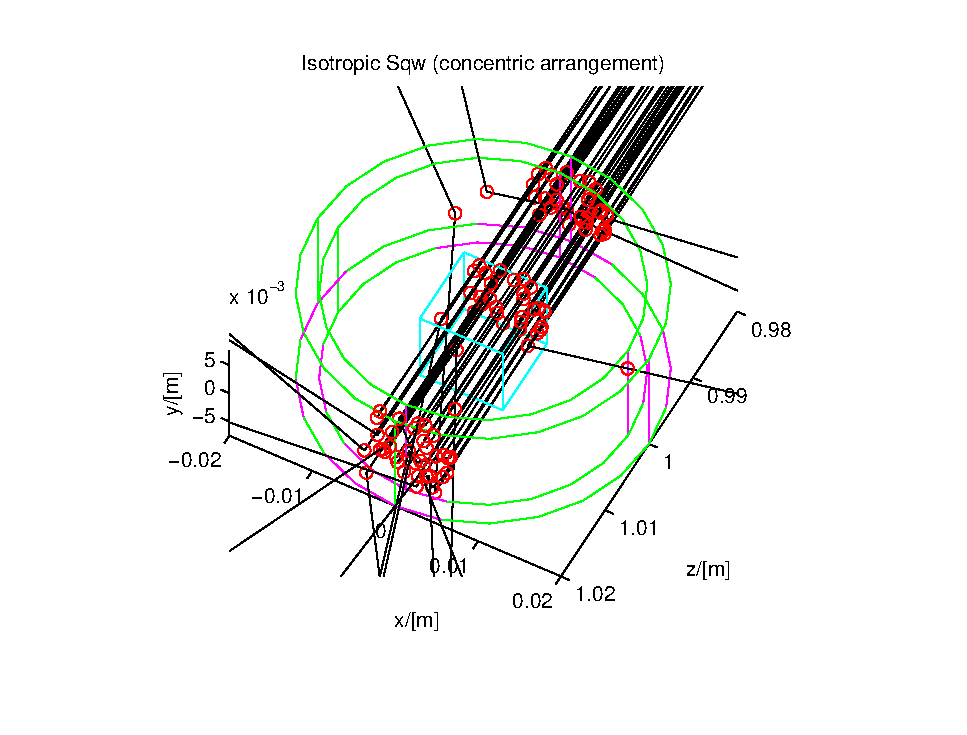
\includegraphics[width=0.9\textwidth]{figures/sqw.eps}
  \end{center}
\caption{An $l-^4$He sample in a cryostat, simulated with the Isotropic\_Sqw component in concentric geometry.}
\label{f:isotropic-sqw}
\end{figure}

The component assumes that the sample has the structure of an isotropic material. This stands for liquids, glasses (amorphous systems), polymers, gaz, and may be extended to powders.

\subsection{Neutron interaction with matter}

When a neutron enters a material, according to usual models and letting the absorption aside to begin with, it 'sees' atoms as disks with a surface equal to the total scattering cross section of material $\sigma$. Each coherent and incoherent process is associated with a given probability to hit these cross-sections, according to $\sigma_{coh}$ or $\sigma_{inc}$. We may choose randomly a scattering position along the path, using e.g. an expeonential decay probability. If the scattering condition is not satisfied, the neutron is transmitted, and leaves the sample. In any case, the absorption lowers the intensity according to an $e^{-\rho \sigma_abs} d$ absorption law along the propagation path. In this process, the neutron is considered to be a particule.

Once the neutron 'knows' that something (terrible) is going to occur, it looks for a possible excitation to interact with. Then we turn to the wave description of the neutron, which interacts with the whole volume. The distribution of excitations, from which derives their relative intensity in the scattered beam, is simply the dynamic structre factor - or scattering law - $S(q,\omega)$. According to the definition of the density of states, we may use $g(\omega)$ as the probability law to scatter at a given energy transfert.

The neutron leaves the scattering point when a suitable $(q, \omega)$ choice has been found to satisfy the conservation laws. The process is iterated until the neutron leaves the volume of the material, eventually producing multiple scattering contributions.

\subsection{Theoretical side}

Following Squires (\cite{squires}, p63), the neutron differential scattering cross section for both coherent and incoherent processes is
\begin{equation}
\frac{d^2\sigma}{d\Omega dE_f} = \frac{\sigma}{4\pi}\frac{k_f}{k_i} N S(q, \omega)
\end{equation}
with usual notations: $N=\rho V$ is the number of atoms in the scattering volume $V$ with density $\rho$, $E_f, E_i, k_f, k_i$ are the energy and wavevectors of final and initial states respectively, and $\sigma$ is the total scattering cross-section. The unit of the dynamical structure factor $S(q,\omega)$ is an inverse energy.

Some easely measureable quantities in a liquid are the \emph{static pair correlation function} $g(r)$ and the \emph{structure factor} $S(q)$, defined as:
\begin{eqnarray}
\rho g(\vec{r}) &=& \frac{1}{N} \sum_{i=1}^N \sum_{j \neq i} \langle \delta(\vec{r}+\vec{r}_i-\vec{r}_j) \rangle \\
S(\vec{q}) &=&\int S(\vec q,\omega) d\omega \\
           &=&1 + \rho \int_V [g(\vec{r})-1] e^{i\vec{q}.\vec{r}} d\vec{r} \\
           &=&1 + \rho \int_{0}^{\infty} [g(r)-1] \frac{\sin(qr)}{qr} 4 \pi r^2 dr {\rm\ in\ isotropic\ materials.}
\end{eqnarray}
Both $g(r)$ and $S(q)$ converge to unity for large $r$ and $q$ values respectively, and they are representative of the atoms spatial distribution. Moreover in a liquid $\lim_{q \rightarrow 0} S(q) = \rho k_B T \chi_T$ where $\chi_T=\frac{\partial \rho}{\partial P}_{V,T}$ is the compressibility \cite{Egelstaff67}. These quantities are obtained experimentaly from diffractometers.

On the other hand, we may measure, usually with time-of-flight instruments, the \emph{density of states} $g(\omega)$  which is the fraction of modes whose energy lie between $\omega$ and $\omega+d\omega$ \cite{lovesey84}
\begin{equation}
g(\omega) = \frac{\int S(q,\omega) dq}{\iint S(q,w) dq, d\omega} .
\end{equation}
This function is normalized to unity, $\int (gh(\omega) d\omega = 1$ and is a probability distribution of mode energies in the material.

The main idea to implement the scattering from $S(q, \omega)$ is to basically make two consecutive Monte Carlo choices, applying the well known \emph{joint probability} theorem:
\begin{equation}
P(q \cap \omega) = P(\omega).P(q \mid \omega) .
\end{equation}

Thus we define $P(\omega)$ as the cumulated distribution of the density of states $g(\omega)$.  $P(\omega)$ is the probability for an excitation to have an energy lower than $\omega$.

Similarly, we define the conditional probability $P((q \mid \omega)$ to be, for each energy lying between $\omega$ and $\omega+d\omega$, the cumulated distribution of the probability
\begin{equation}
\hat g(q,\omega) = \frac{S(q, \omega)}{\int S(q,\omega) dq} .
\end{equation}
$P(q \mid \omega)$ is the probability for an excitation to have a wavevector lower than $q$, for a given energy transfert $\omega$.

\begin{figure}
  \begin{center}
    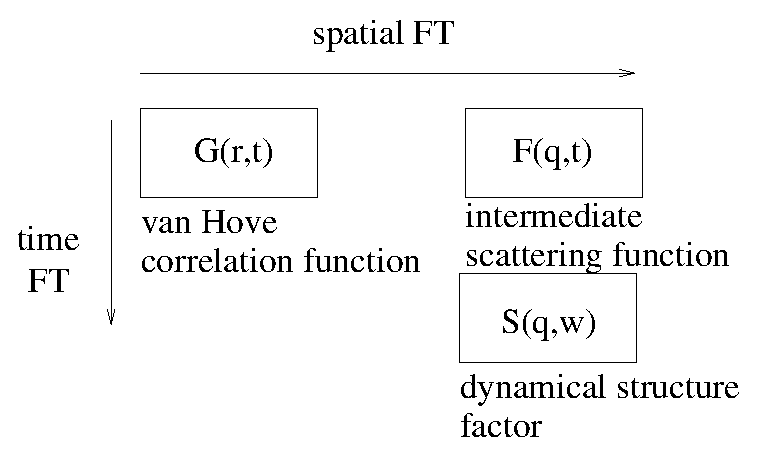
\includegraphics[width=0.9\textwidth]{figures/GFS.eps}
  \end{center}
\caption{The probability functions extracted from $S(q,\omega)$. The energy transfert is first selected from the density of states, then the wavevector is obtained from $\hat g$.}
\label{f:isotropic-sqw}
\end{figure}


\subsection{The implementation}
\subsubsection{Choosing the interaction position}

The probability that the neutron scatters between two positions $x$ and $x+dx$ is given by $\mu e^{-\mu x}dx$, where $\mu = \rho\sigma$ is the linear attenuation. If the straight path to the sample volume exit is $d_{out}$, the probability that the neutron scatters before exiting the sample at a distance $d_{scatt}$ is:
\begin{equation}
P(d_{scatt} < d_{out}) = \int_0^{d_{out}} \mu e^{-\mu x}dx = 1 - e^{-\mu d_{out}}. \\
\end{equation}
Form that law, we may compute the cumulated distribution, which gives the probability for scattering to occur at a distance lower than $d_{scatt}$. This law may be analytically inverted so that the path length $d_{scatt}$ may be obtained directly from a uniform distribution random number $\xi$
\begin{equation}
d_{scatt} = -\frac{1}{\mu} \ln(1 - \xi[1 -e^{-\mu d_{out}}]).
\end{equation}
Then we scale the neutron weight by $1 - e^{-\mu d_{out}}$, in order to account for the fraction of neutrons scattering before exiting the sample.

A similar method is used in the \verb+Single_crystal+ component (section \ref{s:Single_crystal}).


\subsubsection{Choosing the type of interaction}
\subsubsection{Choosing the $q$ and $\omega$ transfert}

% Emacs settings: -*-mode: latex; TeX-master: "manual.tex"; -*-

\chapter{Monitors and detectors}
\index{Library!Components!monitors}

In real neutron experiments, detectors and monitors play quite
different roles. One wants the detectors to be as efficient as
possible, counting all neutrons (absorbing them in the process),
while the monitors measure the intensity of the incoming beam, and must
as such be almost transparent, interacting only with (roughly) 0.1-1\%
of the neutrons passing by. In computer simulations, it is
of course possible to detect every neutron without
absorbing it or disturbing any of its parameters. Hence, the two components
have very similar functions in the simulations, and we do
not distinguish between them. For simplicity, they are from here on
just called monitors, since they do not absorb neutrons.

Another important difference between computer simulations
and real experiments is
that one may allow the monitor to be sensitive to any neutron property,
as {\em e.g.} direction, energy, and divergence, in addition to what
is found in advanced existing monitors (space and time). One may, in
fact, let the monitor have several of these properties at the same time,
as seen for example in the energy sensitive monitor in
section~\ref{s:e_monitor}.

When a monitor detects a neutron ray,
a number counting variable is incremented: $n_i = n_{i-1}+1$
In addition, the neutron
weight $p_i$ is added to the weight counting variable:
$I_i = I_{i-1} + p_i$,
and the second moment of the weight is
updated: $M_{2,i} = M_{2,i-1} + p_i^2$.
As also discussed in the System Manual, after a simulation of $N$ rays
the detected intensity (in units of neutrons/sec.) is $I_N$,
while the estimated errorbar is $\sqrt{M_{2,i}^2}$.


Many different monitor components have been developed for
\MCS , but we have selected to support only the most important ones.
One example of the monitors we have omitted is the single monitor,
{\bf Monitor},
that measures just one number (with errorbars) per simulation.
This effect is mirrored by any of the 1- or 2-dimensional detectors
we support, e.g. the {\rm PSD\_monitor}.
In case additional functionality of monitors is required,
the existing monitors can easily be modified.

However, the ultimate solution is the use of the
``Swiss army knife'' of monitors, {\rm Monitor\_nD}, that can face
almost any simulation challenge.

\newpage
\section{TOF\_monitor: The time-of-flight monitor}
\component{TOF\_monitor}{System}{$x_{\rm min}$, $x_{\rm max}$, $y_{\rm min}$, $y_{\rm max}$, $n_{\rm chan}$, $t_0$, $t_1$, filename}{$\Delta t$}{}
\index{Monitors!Time-of-flight monitor}

The component {\bf TOF\_monitor} has a rectangular opening
in the $(x,y)$ plane, given by the $x$ and $y$ parameters,
like for {\bf Slit}.
The neutron ray is propagated to the plane of the monitor
by the kernel call PROP\_Z0.
A neutron ray is counted if it passes within the rectangular opening
given by the $x$ and $y$ limits.

Special about {\bf TOF\_monitor} is that it is sensitive to
the arrival time, $t$, of the neutron ray.
Like in a real time-of-flight detector, the time dimension is
binned into small time intervals.
Hence this monitor maintains a one-dimensional histogram of counts.
The $n_{\rm chan}$ time intervals begin at $t_0$ and
end at $t_1$ (alternatively, the interval length is specified by $\Delta t$).
As usual in time-of-flight analysis, all times are given in units of $\mu$s.

The output parameters from {\bf TOF\_monitor} are the three count numbers,
$N, I$, and $M_2$ for the total counts in the monitor.
In addition, a file, \verb+filename+, is produced with a list of
the same three data divided in different TOF bins.
This file can be read and plotted by the {\rm mcplot} tool; see the
System Manual.



\newpage
% Emacs settings: -*-mode: latex; TeX-master: "manual.tex"; -*-

\section{E\_monitor: The energy-sensitive monitor}
\index{Monitors!Energy monitor}
\component{E\_monitor}{System}{$x_{\rm min}$, $x_{\rm max}$, $y_{\rm min}$, $y_{\rm max}$, $n_{\rm chan}$, $E_{\rm min}$, $E_{\rm max}$, filename}{}{}

The component {\bf E\_monitor} resembles {\bf TOF\_monitor}
to a very large extent. Only this monitor is sensitive to
the neutron energy, which in binned in \textit{nchan} bins between
$E_{\rm min}$ and $E_{\rm max}$.

The output parameters from {\bf E\_monitor} are the total counts,
and a file with 1-dimensional data: counts vs. $E$ as for {\bf TOF\_monitor}.




\newpage
% Emacs settings: -*-mode: latex; TeX-master: "manual.tex"; -*-


\section{L\_monitor: The wavelength sensitive monitor}
\label{s:L_monitor}

\component{L\_monitor}{System}{$x_{\rm min}$, $x_{\rm max}$, $y_{\rm min}$, $y_{\rm max}$, $n_{\rm chan}$, $\lambda_{\rm min}$, $\lambda_{\rm max}$, filename}{}{}


The component {\bf L\_monitor} is very similar to
{\bf TOF\_monitor} and {\bf E\_monitor}.
Only is this component sensitive to the neutron wavelength.
The wavelength spectrum is output in a one-dimensional histogram.
between $\lambda_{\rm min}$ and $\lambda_{\rm max}$ (measured in \AA ).

As for the two other 1-dimensional monitors, this component outputs
the total counts and a file with the histogram.



\newpage
% Emacs settings: -*-mode: latex; TeX-master: "manual.tex"; -*-

\section{PSD\_monitor: The PSD monitor}
\component{PSD\_monitor}{System}{$x_{\rm min}$, $x_{\rm max}$, $y_{\rm min}$, $y_{\rm max}$, $n_x$, $n_y$, filename}{}{}


The component {\bf PSD\_monitor} resembles other monitors, e.g.
{\bf E\_Monitor}, and also propagates the neutron to the detector
surface in the $(x,y)$-plane, where the detector window is set
by the $x$ and $y$ input coordinates.
The PSD monitor, though, is not sensitive to the neutron energy, but
rather its position. the rectangular monitor window is divided
into $n_x \times n_y$ pixels, each of which acts like a single
counter.

The output from {\bf PSD\_monitor} is the integrated counts, $n, I, M_2$,
as well as
three two-dimensional arrays of counts: $n(x,y), I(x,y), M_2(x,y)$.
The arrays are written to a file and can be read e.g. by the tool
{\bf MC\_plot}, see the system manual.

{\bf Burde man ikke kunne specificere en radius,
og s\aa\ blev den en 2D cylinder detektor??}

\newpage
% Emacs settings: -*-mode: latex; TeX-master: "manual.tex"; -*-

\section{Divergence\_monitor: A divergence sensitive monitor}
\label{s:div-monitor}
\index{Monitors!Divergence monitor}
\component{Divergence\_monitor}{System}{$x_{\rm min}$, $x_{\rm max}$, $y_{\rm min}$, $y_{\rm max}$, $n_{\rm v}$, $n_{\rm h}$, $\eta_{\rm v,max}$, $\eta_{\rm h,max}$, filename}{}{}


The component {\bf Divergence\_monitor} is a two-dimensional monitor,
which resembles {\bf PSD\_Monitor}. As for this component,
the detector window is set
by the $x$ and $y$ input coordinates.
{\bf Divergence\_ monitor} is sensitive to the neutron divergence,
defined by
$\eta_{\rm h} = \tan^{-1}(v_x/v_z)$ and $\eta_{\rm v} = \tan^{-1}(v_y/v_z)$.
The neutron counts are being histogrammed
into $n_{\rm v} \times n_{\rm h}$ pixels. 
The divergence range accepted is in the vertical direction
$[-\eta_{\rm v,max}; \eta_{\rm v,max}]$, and similar for the horizontal
direction.

The output from {\bf PSD\_monitor} is the integrated counts, $n, I, M_2$,
as well as
three two-dimensional arrays of counts: $n(\eta_{\rm v},\eta_{\rm h}),
I(\eta_{\rm v},\eta_{\rm h}), M_2(\eta_{\rm v},\eta_{\rm h})$.
The arrays are written to a file, \verb+filename+, 
and can be read e.g. by the tool {\bf MC\_plot}, see the system manual.


\newpage
\section{DivPos\_monitor: A divergence and position sensitive monitor}
\label{s:divpos-monitor}
\index{Monitors!Divergence/position monitor}
\component{DivPos\_monitor}{System}{$x_{\rm min}$, $x_{\rm max}$, $y_{\rm min}$, $y_{\rm max}$, $n_x$, $n_{\rm h}$, $\eta_{\rm h,max}$, filename}{}{}

{\bf DivPos\_monitor} is a two-dimensional monitor component,
which is sensitive to both horizontal position ($x$) and horizontal divergence
defined by $\eta_{\rm h} = \tan^{-1}(v_x/v_z)$.
The detector window is set
by the $x$ and $y$ input coordinates.

The neutron counts are being histogrammed
into $n_x \times n_{\rm h}$ pixels. The horizontal divergence range accepted is
$[-\eta_{\rm h,max}; \eta_{\rm h,max}]$, and the horizontal position
range is the size of the detector.

The output from {\bf PSD\_monitor} is the integrated counts, $n, I, M_2$,
as well as
three two-dimensional arrays of counts: $n(x,\eta_{\rm h}),
I(x,\eta_{\rm h}), M_2(x,\eta_{\rm h})$.
The arrays are written to a file and can be read e.g. by the tool
{\bf mcplot}, see the system manual.

This component can be used for measuring acceptance diagrams \cite{Cussen03}.
{\bf PSD\_monitor} can easily be changed into being sensitive
to $y$ and vertical divergence by a 90 degree rotation around the $z$-axis.


\newpage
\section{Monitor\_nD: A general Monitor for 0D/1D/2D records}
\label{s:monitornd}
\index{Monitors!The All-in-One monitor (Monitor\_nD)}

\component{Monitor\_nD}{System, E. Farhi}{$x_{\rm min}$, $x_{\rm max}$, $y_{\rm min}$, $y_{\rm max}$, options}{$file$, $x_{width}, y_{height}, z_{depth}$, $bins$, $min$, $max$}{}

The component {\bf Monitor\_nD} is a general Monitor that may output any
set of physical parameters regarding the passing neutrons. The
generated files are either a set of 1D signals ([Intensity] {\it vs.}
[Variable]), or a single 2D signal ([Intensity] {\it vs.} [Variable 1]
{\it vs.} [Variable 1]), and possibly a simple long list of selected
physical parameters for each neutron.

The input parameters for {\bf Monitor\_nD} are its dimensions $x_{\rm
  min}, x_{\rm max}, y_{\rm min}$, $y_{\rm max}$ (in meters) and an {\it
  options} string describing what to detect, and what to do with the
signals, in clear language. The $x_{width}, y_{height}, z_{depth}$ may also be used to enter dimensions.

Eventhough the possibilities of Monitor\_nD are numerous, its usage remains as simple as possible, specially in the \verb+options+ parameter, which 'understands' normal language.
The formatting of the {\it options}
parameter is free, as long as it contains some specific keywords, that
can be sometimes followed by values. The {\it no} or {\it not} option
modifier will revert next option. The {\it all} option can also affect a
set of monitor configuration parameters (see below).

As the usage of this component enables to monitor virtually anything, and thus the combinations of options and parameters is infinite, we shall only present the most basic configuration. The reader should refer to the on-line component help, using e.g. \verb+mcdoc Monitor_nD.comp+.

\subsection{The Monitor\_nD geometry}

The monitor shape can be selected among seven geometries:
\begin{enumerate}
\item{({\it square}) The default geometry is flat rectangular in ($xy$)
    plane with dimensions $x_{\rm min}, x_{\rm max}, y_{\rm min}$,
    $y_{\rm max}$, or $x_{width}, y_{height}$.}
\item{({\it box}) A rectangular box with dimensions $x_{width}, y_{height}, z_{depth}$.}
\item{({\it disk}) When choosing this geometry, the detector is a flat
    disk in ($xy$) plane. The radius is then
    \begin{equation}
      \mbox{radius} = \max ( \mbox{abs } [ x_{\rm min}, x_{\rm max}, y_{\rm
        min}, y_{\rm max}, x_{width}/2, y_{height}/2 ] ).
    \end{equation}
    }
\item{({\it sphere}) The detector is a sphere with the same radius as
    for the {\it disk} geometry.}
\item{({\it cylinder}) The detector is a cylinder with revolution axis
    along $y$ (vertical). The radius in ($xz$) plane is
    \begin{equation}
      \mbox{radius} =  \max ( \mbox{abs } [ x_{\rm min}, x_{\rm max}, x_{width}/2 ] ),
    \end{equation}
    and the height along $y$ is
    \begin{equation}
      \mbox{height} =  | y_{\rm max} - y_{\rm max} | {\rm or} y_{height}.
    \end{equation}
    }
\item{({\it banana}) The same as the cylinder, but without the top/bottom caps, and on a restricted angular range. The angular range is specified using a \verb+theta+ variable limit specification in the \verb+options+.}
\item{({\it previous}) The detector has the shape of the previous component. This may be a surface or a volume. In this case, the neutron is detected on previous component, and there is not neutron propagation.}
\end{enumerate}

By default, the monitor is flat, rectangular. Of course, you can choose
the orientation of the {\bf Monitor\_nD} in the instrument description
file with the usual \texttt{ROTATED} modifier.

For the {\it box}, {\it sphere} and {\it cylinder}, the outgoing neutrons are
monitored by default, but you can choose to monitor incoming neutron
with the {\it incoming} option.

At last, the {\it slit} or {\it absorb} option will ask the component to
absorb the neutrons that do not intersect the monitor. The {\it exclusive} option word removes neutrons which are similarly outside the monitor limits (that may be other than geometrical).

The {\it parallel} option keyword is of common use in the case where the {\bf Monitor\_nD} is superposed with other components. It ensures that neutrons are detected independently of other geometrical constrains. This is generally the case when you need e.g. to place more than one monitor at the same place.

\subsection{The neutron parameters that can be monitored}

There are many different variables that can be monitored at the same time
and position. Some can have more than one name (e.g. \texttt{energy} or
\texttt{omega}).


\begin{verbatim}
    kx ky kz k wavevector [Angs-1] (    usually axis are
    vx vy vz v            [m/s]         x=horz., y=vert., z=on axis)
    x y z                 [m]      Distance, Position
    kxy vxy xy radius     [m]      Radial wavevector, velocity and position
    t time                [s]      Time of Flight
    energy omega          [meV]
    lambda wavelength     [Angs]
    p intensity flux      [n/s] or [n/cm^2/s]
    ncounts               [1]
    sx sy sz              [1]      Spin
    vdiv ydiv dy          [deg]    vertical divergence (y)
    hdiv divergence xdiv  [deg]    horizontal divergence (x)
    angle                 [deg]    divergence from  direction
    theta longitude       [deg]    longitude (x/z) [for sphere and cylinder]
    phi   lattitude       [deg]    lattitude (y/z) [for sphere and cylinder]
\end{verbatim}
as well as two other special variables
\begin{verbatim}
    user user1            will monitor the [Mon_Name]_Vars.UserVariable{1|2}
    user2 user3           to be assigned in an other component (see below)
\end{verbatim}

To tell the component what you want to monitor, just add the variable
names in the {\it options} parameter. The data will be sorted into {\it
  bins} cells (default is 20), between some default {\it limits}, that
can also be set by user. The {\it auto} option will automatically
determine what limits should be used to have a good sampling of signals.

\subsection{Important options}

Each monitoring records the flux (sum of weights $p$) versus the
given variables, except if the \verb+signal=<variable>+ word is used in the \verb+options+.
The {\it cm2} option will ask to normalize the flux to the monitor section surface, and the \verb+capture+ option uses the gold foil integrated 'capture' flux weightening (up to the cadmium cut-off):\index{Monitors!Capture flux}
\begin{equation}
\Phi_c = \int_0^{0.5 eV}{\frac{d\Phi}{d\lambda} \frac{\lambda}{\lambda_{2200 m/s}} d\lambda}
\end{equation}

The \verb+auto+ option is probably the most useful one: it asks the monitor to determine automatically the best limits for each variable, in order to obtain the most significant monitored histogram. This option should preceed each variable, or be located after all variables in which case they are all affected.
On the other hand, one may manually set the limits with the \verb+limits=[min max]+ option.

The \verb+log+ and \verb+abs+ options should be positioned before each variable to specify logarithmic binning and absolute value respectively.

The {\it borders} option will monitor variables that are outside
the limits. These values are then accumulated on the 'borders' of the
signal.

\subsection{The output files}

By default, the file names will be the component name, followed by a time stamp and
automatic extensions showing what was monitored (such as
\texttt{MyMonitor.x}). You can also set the filename in {\it options}
with the {\it file} keyword followed by the file name that you want. The
extension will then be added if the name does not contain a dot (.).
Finally, the $filename$ parameter may also be used.

The output files format are standard 1D or 2D McStas detector files.
The {\it no file} option will {\it unactivate} monitor, and make it a
single 0D monitor detecting integrated flux and counts.
The {\it verbose} option will display the nature of the monitor, and the
names of the generated files.

\subsubsection{The 2D output}

When you ask the {\bf Monitor\_nD} to monitor only two variables (e.g.
{\it options} = "x y"), a single 2D file of intensity versus these two
correlated variables will be created.

\subsubsection{The 1D output}

The {\bf Monitor\_nD} can produce a set of 1D files, one for each
monitored variable, when using 1 or more than 2 variables, or when
specifying the {\it multiple} keyword option.

\subsubsection{The List output}

The {\bf Monitor\_nD} can additionally produce a {\it list} of variable
values for neutrons that pass into the monitor. This feature is additive
to the 1D or 2D output. By default only 1000 events will be recorded in
the file, but you can specify for instance "{\it list} 3000 neutrons" or
"{\it list all} neutrons". This last option might require a lot of
memory and generate huge files.

\subsection{Monitor equivalences}

In the following table \ref{t:monitor-nd-equiv}, we show how the Monitor\_nD may substitute any other \MCS monitor.

\begin{table}
  \begin{center}
    {\let\my=\\
    \begin{tabular}{|p{0.24\textwidth}|p{0.7\textwidth}|}
\hline
\MCS monitor & Monitor\_nD equivalent \\
\hline
Divergence\_monitor & {\it options}="dx bins=$ndiv$ limits=[$-\alpha/2 \alpha/2$],
                                lambda bins=$nlam$ limits=[$\lambda_0$ $\lambda_1$] file=$file$"\\
DivLambda\_monitor  & {\it options}="dx bins=$nh$   limits=[$-h_{max}/2 h_{max}/2$],
                                    dy bins=$nv$   limits=[$-v_{max}/2 v_{max}/2$]" {\it filename}=$file$\\
DivPos\_monitor     & {\it options}="dx bins=$ndiv$ limits=[$-\alpha/2 \alpha/2$],
                                     x bins=$npos$" {\it xmin}=$x_{min}$ {\it xmax}=$x_{max}$ \\
E\_monitor          & {\it options}="energy bins=$nchan$ limits=[$E_{min} E_{max}$]" \\
EPSD\_monitor       & {\it options}="energy bins=$n_E$ limits=[$E_{min} E_{max}$], x bins=$nx$"
                              {\it xmin}=$x_{min}$ {\it xmax}=$x_{max}$ \\
Hdiv\_monitor       & {\it options}="dx bins=$nh$ limits=[$-h_{max}/2 h_{max}/2$]" {\it filename}=$file$ \\
L\_monitor          & {\it options}="lambda bins=$nh$ limits=[$-\lambda_{max}/2 \lambda_{max}/2$]" {\it filename}=$file$ \\
Monitor\_4PI        & {\it options}="sphere" \\
Monitor            & {\it options}="unactivate" \\
PSDcyl\_monitor     & {\it options}="theta bins=$nr$,y bins=$ny$, cylinder"
{\it filename}=$file$ {\it yheight}=$height$ {\it xwidth}=2*radius\\
PSDlin\_monitor     & {\it options}="x bins=$nx$" {\it xmin}=$x_{min}$ {\it xmax}=$x_{max}$ {\it ymin}=$y_{min}$ {\it ymax}=$y_{max}$ {\it filename}=$file$\\
PSD\_monitor\_4PI    & {\it options}="theta y, sphere" \\
PSD\_monitor        & {\it options}="x bins=$nx$, y bins=$ny$" {\it xmin}=$x_{min}$ {\it xmax}=$x_{max}$ {\it ymin}=$y_{min}$ {\it ymax}=$y_{max}$ {\it filename}=$file$\\
TOF\_cylPSD\_monitor & {\it options}="theta bins=$n_\phi$, time bins=$nt$ limits=[$t_0, t_1$], cylinder" {\it filename}=$file$ {\it yheight}=$height$ {\it xwidth}=2*radius\\
TOFLambda\_monitor  & {\it options}="lambda bins=$n_\lambda$ limits=[$\lambda_0$ $\lambda_1$], time bins=$nt$ limits=[$t_0, t_1$]" {\it filename}=$file$\\
TOFlog\_mon         & {\it options}="log time bins=$nt$ limits=[$t_0, t_1$]" \\
TOF\_monitor        & {\it options}="time bins=$nt$ limits=[$t_0, t_1$]" \\
\hline
    \end{tabular}
    \caption{Using Monitor\_nD in place of other components. All limits specifications may be advantageously replaced by an {\it auto} word preceeding each monitored variable. Not all file and dimension specifications are indicated (e.g. filename, xmin, xmax, ymin, ymax).}
    \label{t:monitor-nd-equiv}
    }
  \end{center}
\end{table}

\subsection{Usage examples}

\begin{itemize}
\item{
\begin{verbatim}
COMPONENT MyMonitor = Monitor_nD(
    xmin = -0.1, xmax = 0.1,
    ymin = -0.1, ymax = 0.1,
    options = "energy auto limits")
\end{verbatim}
will monitor the neutron energy in a single 1D file (a kind of E\_monitor)}
\item{\texttt{options = "banana, theta limits=[10,130], bins=120, y bins=30"} \\
    is a theta/height banana detector.\index{Monitors!Banana shape}}
\item{\texttt{options = "banana, theta limits=[10,130], auto time"} \\
    is a theta/time-of-flight banana detector.}

\item{\texttt{options="x bins=30 limits=[-0.05 0.05] ; y"} \\
    will set the monitor to look at $x$ and $y$. For $y$, default bins (20)
    and limits values (monitor dimensions) are used.}

\item{\texttt{options="x y, auto, all bins=30"} \\
    will determine itself the required limits for $x$ and $y$.}

\item{\texttt{options="multiple x bins=30, y limits=[-0.05 0.05], all auto"} \\
will monitor the neutron $x$ and $y$ in two 1D files.}
\item{\texttt{options="x y z kx ky kz, all auto"} \\
will monitor each of theses variables in six 1D files.}
\item{\texttt{options="x y z kx ky kz, list all, all auto"} \\
will monitor all theses neutron variables in one long list, one row per neutron event.}
\item{\texttt{options="multiple x y z kx ky kz, and list 2000, all auto"} \\
    will monitor all theses neutron variables in one list of 2000 events
    and in six 1D files.}
\item{\texttt{options="signal=energy, x y"} \\
    is a PSD monitor recording the mean energy of the beam as a function of $x$ and $y$.\index{Monitors!Position sensitive monitor recording mean energy}}
\end{itemize}

\subsection{Monitoring user variables}
\label{s:monnd:user}
\index{Monitors!Custom monitoring (user variables, Monitor\_nD)}

There are two ways to monitor any quantity with Monitor\_nD. This may be e.g. the number of neutron bounces in a guide, or the wavevector and energy transfer at a sample. The only requirement is to define the \verb+user1+ (and optionally \verb+user2,user3+) variables of a given Monitor\_nD instance.

\subsubsection{Setting directly the user variables (simple)}

The first method uses directly the \verb+user1+ and \verb+username1+ component parameters to transfert directly the value and label, such as in the following example:
\begin{verbatim}
TRACE
(...)
COMPONENT UserMonitor = Monitor_nD(
  user1    = log(t), username1="Log(time)",
  options  ="auto user1")
\end{verbatim}
The values to assign to \verb+user2+ and \verb+user3+ must be global instrument variables, or a component output variables as in \verb+user1=MC_GETPAR(some_comp, outpar)+.
Similarly, the \verb+user2,user3+ and \verb+username2,username3+ parameters may be used to control the second and third user variable, to produce eventually 2D/3D user variable correlation data and custom event lists.

\subsubsection{Setting indirectly the user variables (only for professionals)}

It is possible to control the user variables of a given Monitor\_nD instance anywhere in the instrument description. This method requires more coding, but has the advantage that a variable may be defined to store the result of a computation locally, and then transfert it into the UserMonitor, all fitting in an EXTEND block.

This is performed in a 4 steps process:
\begin{enumerate}
\item Declare that you intend to monitor user variables in a Monitor\_nD instance (defined in TRACE):
\begin{verbatim}
DECLARE
%{ (...)
  %include "monitor_nd-lib"
  MONND_DECLARE(UserMonitor); // will monitor custom things in UserMonitor
%}
\end{verbatim}
\item Initialize the label of the user variable (optional):
\begin{verbatim}
INITIALIZE
%{
  (...)
  MONND_USER_TITLE(UserMonitor, 1, "Log(time)");
%}
\end{verbatim}
The value '1' could be '2' or '3' for the \verb+user2,user3+ variable.
\item Set the user variable value in a TRACE component EXTEND block:\index{Keyword!EXTEND}
\begin{verbatim}
TRACE
(...)
COMPONENT blah = blah_comp(...)
EXTEND
%{  // attach a value to user1 in UserMonitor, could be much more comlex here.
  MONND_USER_VALUE(UserMonitor, 1, log(t));
%}
(...)
\end{verbatim}
\item Tell the Monitor\_nD instance to record user variables:
\begin{verbatim}
TRACE
(...)
COMPONENT UserMonitor = Monitor_nD(options="auto user1")
(...)
\end{verbatim}
\end{enumerate}
Setting the user variable values may either make use of the neutron parameters (x,y,z, vx,vy,vz, t, sx,sy,sz, p), access the internal variables of the component that sets the user variables (in this example, those from the \verb+blah+ instance), access any component OUTPUT parameter \index{Keyword!OUTPUT PARAMETERS} using the \verb+MC_GETPAR+ C macro(see chapter \ref{c:kernelcalls}), or simply use a global instrument variable. Instrument parameters can not be used directly.
\index{Library!Run-time!MC\_GETPAR}

\subsubsection{Example: Number of neutron bounces in a guide}

\index{Monitors!Number of neutron bounces in a guide}
In the following example, we show how the number of bounces in a polygonal guide may be monitored. Let us have a guide made of many Guide\_gravity instances. We declare a global simulation variable \verb+nbounces+, set it to 0 for each neutron entering the guide, and sum-up all bounces from each section, accessing the \verb+Gvars+ OUTPUT variable of component Guide\_gravity. Then we ask Monitor\_nD to look at that value.
\begin{verbatim}
DECLARE
%{
  double nbounces;
%}
TRACE
(...)
COMPONENT Guide_in = Arm() AT (...)
EXTEND
%{
  nbounces = 0;
%}

COMPONENT Guide1 = Guide_gravity(...) AT (...) RELATIVE PREVIOUS
EXTEND
%{
  if (SCATTERED) nbounces += GVars.N_reflection[0];
%}
(... many guide instances, copy/paste and change names automatically ...)
COMPONENT COPY(Guide1) = COPY(Guide1) AT (...) RELATIVE PREVIOUS
EXTEND
%{
  if (SCATTERED) nbounces += GVars.N_reflection[0];
%}

// monitor nbounces
COMPONENT UserMonitor = Monitor_nD(
  user1=nbounces, username1="Number of bounces",
  options="auto user1") AT (...)
(...)
\end{verbatim}

\subsection{Monitoring neutron parameter correlations, PreMonitor\_nD}

The first imediate usage of the Monitor\_nD component is when one requires to identify cross-correlations between some neutron parameters, e.g. position and divergence ({\it aka} phase-space diagram). This latter monitor would be merely obtained with:\index{Monitors!Neutron parameter correlations, PreMonitor\_nD}
\begin{verbatim}
options="x dx, auto", bins=30
\end{verbatim}
This example records the correlation between position and divergence of neutrons at a given instrument location.

\component{PreMonitor\_nD}{System, E. Farhi}{comp}{}{}

But it is also possible to search for cross-correlation between two part of the instrument simulation. One example is the acceptance phase-diagram, which shows the neutron caracteristics at the input required to reach the end of the simulation. This \emph{spatial} correlation may be revealed using the {\bf PreMonitor\_nD} component. This latter stores the neutron parameters at a given instrument location, to be used at an other Monitor\_nD location for monitoring.

The only parameter of {\bf PreMonitor\_nD} is the name of the associated Monitor\_nD instance, which should use the \verb+premonitor+ option, as in the following example:
\begin{verbatim}
COMPONENT CorrelationLocation = PreMonitor_nD(comp = CorrelationMonitor)
AT (...)

  (... e.g. a guide system )

COMPONENT CorrelationMonitor  = Monitor_nD(
   options="x dx, auto, all bins=30, premonitor")
AT (...)
\end{verbatim}
which performs the same monitoring as the previous example, but with a spatial correlation constrain. Indeed, it records the position {\it vs} the divergence of neutrons at the correlation location, but only if they reach the monitoring position. All usual Monitor\_nD variables may be used, except the user variables. These latter may be defined as described in section \ref{s:monnd:user} in an EXTEND block.


%\newpage
%\input{monitor_nd}
\chapter{Special-purpose components}
\index{Library!Components!misc}

The chapter deals with components that are not easily included
in any of the other chapters because of their special nature,
but which are still part of the \MCS\ system.

One part of these components deals with splitting simulations
into two (or more) stages. For example, a guide system is often
not changed much, and a long simulation of neutron rays
``surviving'' through the guide system could be reused
for several simulations of the instrument back-end, speeding up
the simulations by (typically) one or two orders of magnitude.
The components for doing this trick is {\bf Virtual\_input} and
{\bf Virtual\_output}, which stores and reads neutron rays, respectively.

Another pair of components performs the simulation of the instrument
resolution functions. This is {\bf Res\_sample} and {\bf TOF\_Res\_sample}, 
which are to be
placed at the sample position, and {\bf Res\_monitor}, that should
be localized at the position of the instrument detector.

{\bf Progress\_bar} is a simulation utility that displays the simulation
status, but assumes the form of a component.

\newpage
\section{Vitual\_output: Saving the first part of a split simulation}
\label{virtual_output}
\index{Sources!Virtual source, recording neutron events}

\component{Virtual\_output}{System}{filename}{buffer-size, type}{}

The component {\bf Virtual\_output} stores the neutron ray parameters
at the end of the first part of a split simulation. The idea is to let the
next part of the split simulation be performed by another instrument file,
which reads the stored neutron ray
parameters by the component {\bf Virtual\_input}.

All neutron ray parameters are saved to the output file, which is by default
of ``text'' type, but can also assume the binary formats
``float'' or ``double''. The storing of neutron rays continue until the
specified number of simulations have been performed.

\verb+buffer-size+ may be used to limit the size of the output file, but 
absolute intentities are then likely to be wrong. 
We recommend to use the default value of zero, saving all neutron rays. 
The size of the file is then controlled indirectly with 
the general $ncounts$ parameter.


\newpage
\section{Vitual\_input: Starting the second part of a split simulation}
\label{virtual_input}
\index{Sources!Virtual source from stored neutron events}

\component{Virtual\_input}{System}{filename}{repeat-count, type}{}

The component {\bf Virtual\_input} resumes a split simulation where the
first part has been performed by another instrument and the neutron ray
parameters have been stored by the component {\bf Virtual\_output}.

All neutron ray parameters are read from the input file, which is by default
of ``text'' type, but can also assume the binary formats
``float'' and ``double''. The reading of neutron rays continue until the
specified number of rays have been simulated or
till the file has been exhausted. If desirable, the input file
can be reused a number of times, determined by the optional parameter
``repeat-count''. This is only useful if the present simulation makes use of
MC choices, otherwise the same outcome will result for each repetition of the
simulation (see Appendix \ref{s:MCtechniques}).

Care should be taken when dealing with
absolute intensities, which will be correct only
when the input file has been exhausted at least once.

The simulation ends with either the end of the repeated file counts,
or with the normal end with $ncount$ \MCS\ simulation events. We recommand to
control the simulation on \verb+repeat-count+ by using
a very larger ncount value.


\newpage
\section{Res\_sample: A sample-like component for resolution calculation}
\label{s:res_sample}
\index{Samples!Resolution function, sample for}

\component{Res\_sample}{(System); Alan Tennant, HMI}{$r$, $r$, $h$, $r_{\rm focus}$, $x_{\rm target}$, $y_{\rm target}$, $z_{\rm target}$, $E_0$, $\Delta E$ }{$x_w$, $y_h$, $z_d$, $x_{\rm focus}$, $y_{\rm focus}$, $a_{\rm v, focus}$, $a_{\rm h, focus}$, target index}{}

The component \textbf{Res\_sample} scatters neutron rays isotropically
in direction and uniformly in energy.
Regardless of the state of the incoming neutron ray,
all directions and energies for the scattered ray have the same probability,
within specified intervals.

The component is meant
for computation of the resolution function, but may also be used
for test and debugging purposes. For actual calculations of the resolution
function, {\bf Res\_sample} should be used
together with \textbf{Res\_monitor}, described in
section~\ref{s:res_monitor}.

The shape of {\rm Res\_sample} is either a hollow cylinder
or a rectangular box.
The hollow cylinder shape is
specified with the outer radius, $r$ and thickness,
respectively, and the height, $h$.
If these parameters are unspecified,
the shape is instead a box of dimensions $x_w$, $y_h$, and $z_d$.
%
%\begin{figure}[htbp]
%  \begin{center}
%        \psfrag{ri}[c][c]{\textit{radius\_i}}
%        \psfrag{ro}[c][c]{\textit{radius\_o}}
%        \psfrag{h}[c][c]{\textit{h}}
%        \psfrag{bri}[c][c]{\textit{radius\_i}}
%        \psfrag{bro}[c][c]{$-\textit{radius\_o}$}
%        \psfrag{bh}[c][c]{\textit{h}}
%        \psfrag{X}[c][c]{\textit{X}}
%        \psfrag{Y}[c][c]{\textit{Y}}
%        \psfrag{Z}[c][c]{\textit{Z}}
%        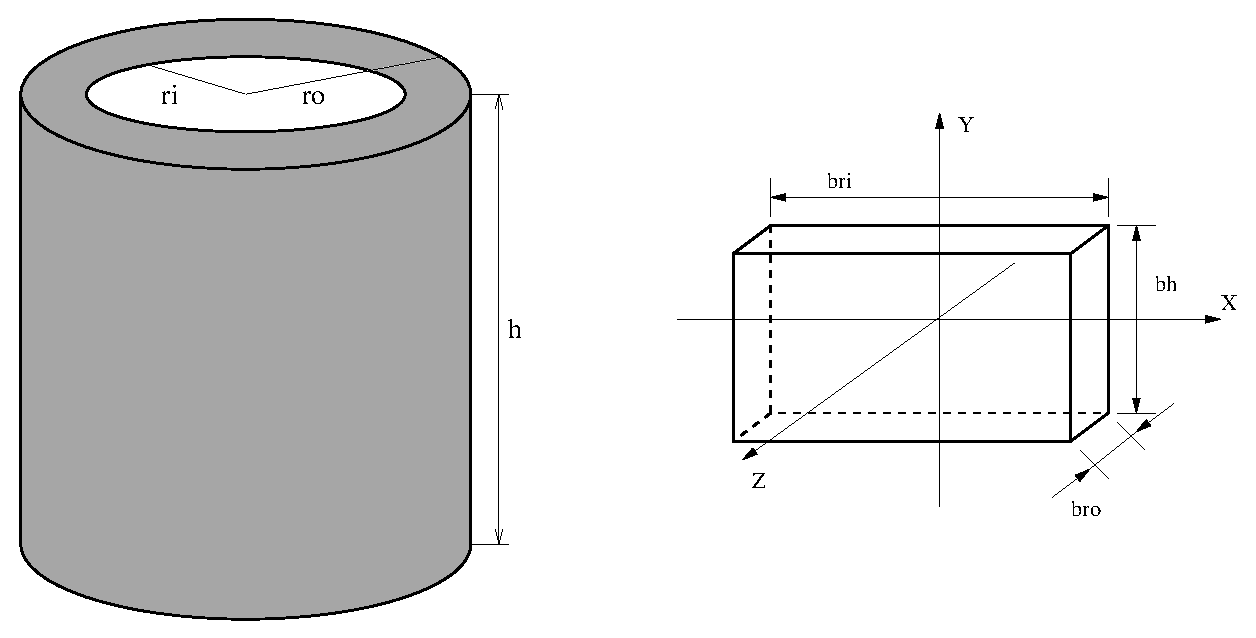
\includegraphics[width=0.9\textwidth]{figures/res_sample.eps}
%    \caption{The two possible shapes of the \textbf{Res\_sample} component.}
%    \label{f:res_sample}
%  \end{center}
%\end{figure}
%
The component only propagates neutron rays that are scattered;
other rays are absorbed. The scattering probability is proportional to the neutron
flight path length inside the sample, to make a true volume weighting
of the sample. The reason for this is that the resolution
function of an instrument is independent of any sample properties
such as scattering and absorbtion cross sections but will in general
depend on sample size and shape.

The point of scattering inside the sample is chosen uniformly
along the neutron flight path inside the sample, and the scattered
neutron ray is given a random energy and direction. This energy is selected in
the interval $[E_0-\Delta E; E_0+\Delta E]$ which hence must be
chosen large enough to cover all interesting neutron energies.
Similarly, the scattered
direction is chosen in a user-specified range,
either within a sphere of radius $r_{\rm focus}$, within a rectangular
target with measures $(x_{\rm focus}, y_{\rm focus})$
or in the specified angular range. This target is positioned at the $x_{target}$, $y_{target}$, $z_{target}$ point in space, or using the target\_index for which e.g. 1 is the further component, -1 is the previous, etc...

A special feature, used when computing resolution functions, is that the
component stores complete information about the scattering event in the
output parameter \textit{res\_struct}. The information includes initial
and final wave vectors, the coordinates of the scattering point, and the
neutron weight after the scattering event. From this information the
scattering parameters $({\bf Q}, \omega)$ can be recorded
for every scattering event and used to compute the resolution function.
For an example of using the
information in the output parameter, see the description of the
\textbf{Res\_monitor} component in section~\ref{s:res_monitor}.



\newpage
% Emacs settings: -*-mode: latex; TeX-master: "manual.tex"; -*-

\section{TOF\_Res\_sample: A sample-like component for TOF resolution calculation}
\label{s:tof_res_sample}

\component{TOF\_Res\_sample}{System}{$r_{\rm i}$, $r_{\rm o}$, $h$, $r_{\rm focus}$, $x_{\rm target}$, $y_{\rm target}$, $z_{\rm target}$, $t_0$, $\Delta t$ }{$x_w$, $y_h$, $z_t$, $x_{\rm focus}$, $y_{\rm focus}$, $a_{\rm v, focus}$, $a_{\rm h, focus}$, target index}{}

The component \textbf{TOF\_Res\_sample} scatters neutron rays isotropically
in position within a specified angular range. 
As for {\bf Res\_sample}, this component is meant
for computation of the resolution function, but in this case for one time bin in a
time-of-flight (TOF) instrument. The component selects uniformly the neutron 
energy so that neutron arrival time at the TOF detector lies within one time bin,
specified by $t_0$ and $\Delta t$.
For actual calculations of the resolution
function, {\bf TOF\_Res\_sample} should be used
together with the \textbf{Res\_monitor} component, described in
section~\ref{s:res_monitor}.

The shape of {\rm TOF\_Res\_sample} is either a hollow cylinder
or a rectangular box. 
The hollow cylinder shape is
specified with the inner and outer radius, $r_{\rm i}$ and $r_{\rm o}$,
respectively, and the height, $h$.
If these parameters are unspecified,
the shape is instead a box of dimensions $x_w$, $y_h$, and $z_t$.
See figure~\ref{f:res_sample}.\par

The component only propagates neutron rays that are scattered; 
other rays are absorbed. 
As for {\bf Res\_sample}, the scattering probability is proportional to the neutron
flight path length inside the sample.
The point of scattering in the sample is chosen uniformly
along the neutron flight path inside the sample, and the scattered
direction is chosen in a user-specified range,
either within a sphere of radius $r_{\rm foc}$, within a rectangular
target with measures $(x_{\rm focus}, y_{\rm focus})$
or in the specified angular range. 
This target is positioned at the $x_{target}$, $y_{target}$, $z_{target}$ 
point in space, or using target\_index.

This component stores complete information about the scattering event in the
output parameter \textit{res\_struct}, see {\bf Res\_Sample}. 


\newpage
% Emacs settings: -*-mode: latex; TeX-master: "manual.tex"; -*-

\section{Res\_monitor: The monitor for resolution calculation}
\label{s:res_monitor}
\index{Monitors!Resolution monitor|see{Samples/Resolution function}}

\component{Res\_monitor}{(System); Alan Tennant, HMI}{$x_{\rm min}$, $x_{\rm max}$, $y_{\rm min}$, $y_{\rm max}$, filename, res\_sample, buffer size}{$x_w$, $y_h$, $z_t$, options}{}

The component {\bf Res\_monitor} is used for calculating the
resolution function of a particular instrument with detector of the
shape, size, and position as {\bf Res\_monitor}.
The shape of {\rm Res\_monitor} is by default rectangular,
but can be a box, a sphere, a disk, or a cylinder,
depending on the parameter ``options''.
The component works like a normal single detector, but
also records all scattering events and stores
them to a file that can later be read by 
the \MCS\ frontend tool \verb+mcresplot+.

For time-of-flight (TOF) instruments, {Res\_monitor} should be understood 
as giving the resolution of one time bin of the TOF-detector only; 
the bin properties being specified in the preceding {\bf TOF\_Res\_sample}.

As described in section~\ref{s:res_sample},
the {\bf Res\_monitor} should be used in connection with one of the
components {\bf Res\_sample} or {\bf TOF\_Res\_sample}, 
the name of which should be passed as an
input parameter to \textbf{Res\_monitor}. For example
\begin{verbatim}
    COMPONENT mysample = Res_sample( ... )
    ...
    COMPONENT det = Res_monitor(res_sample_comp = mysample, ...)
    ...
\end{verbatim}

The output file is in ASCII format, one line per scattering event, with
the following columns:
\begin{enumerate}
\item ${\bf k}_{\rm i}$, the three components of the initial wave vector.
\item ${\bf k}_{\rm f}$, the three components of the final wave vector.
\item ${\bf r}$, the three components of the position of the scattering
  event in the sample.
\item $p_{\rm i}$, the neutron weight just after the scattering event.
\item $p_{\rm f}$, the relative neutron weight adjustment from sample to
  detector (so the total weight in the detector is $p_{\rm i}p_{\rm f}$).
\end{enumerate}
From ${\bf k}_{\rm i}$ and ${\bf k}_{\rm f}$, we may compute ${\bf Q} =
{\bf k}_{\rm i} - {\bf k}_{\rm f}$ and $\omega 
= \hbar^2/(2 m_{\rm n})({\bf k}_{\rm i}^2 - {\bf k}_{\rm f}^2)$.
The vectors are given in the local coordinate system of the resolution
sample component. The wave vectors are in units of $\mbox{\AA}^{-1}$, the
energy transfer in meV.

The output parameters from {\bf Res\_monitor}
are the three count numbers, \textit{Nsum}, \textit{psum},
and \textit{p2sum}, and the handle \textit{file} of the output file.


\newpage
\section{Progress\_bar: Simulation progress and automatic saving}
\component{Progress\_bar}{System}{percent, flag\_save}{}{}
\label{s:progress-bar}
\index{Simulation progress bar}

This component displays the simulation progress and status
but does not affect the neutron parameters. 
The display is updated in regular intervals of the full simulation;
the default step size is 10 \%, but it may be changed using 
the \verb+percent+ parameter (from 0 to 100). 
The estimated computation time is displayed at the begining 
and actual simulation time is shown at the end.

Additionally, setting the \verb+flag_save+ to 1 results in 
a regular save of the data files during the simulation. 
This means that is is possible to view the data before the end 
of the computation, and have also a trace of it in case of 
computer crash. The advancement level is stored in these temporary 
data files. Technically, this save is equivalent to sending regularly 
a USR2 signal to the running simulation.


\appendix
% Emacs settings: -*-mode: latex; TeX-master: "manual.tex"; -*-

\chapter{Libraries and conversion constants}
\label{c:kernelcalls}
\index{Library|textbf}
\index{Library!Shared|see{Library/Components/share}}
\index{Library!mcstas-r|see{Library/Run-time}}

The \MCS\ Library contains a number of built-in functions
and conversion constants which are useful when constructing
components. These are stored in the \verb+share+ directory of
the \verb+MCSTAS+ library. \index{Library!Components!share}
\index{Environment variable!MCSTAS}

Within these functions, the 'Run-time' part is available for all
component/instrument descriptions. The other parts
% (see table~\ref{t:comp-share})
are dynamic, that is they are not
pre-loaded, but only imported once when a component requests it
using the \verb+%include+ \MCS\ keyword. For instance, within a
component C code block, (usually SHARE or DECLARE):
\index{Keyword!\%include}
\begin{verbatim}
    %include "read_table-lib"
\end{verbatim}
will include the 'read\_table-lib.h' file, and the 'read\_table-lib.c'
(unless the \verb+--no-runtime+ option is used with \verb+mcstas+).
Similarly,
\begin{verbatim}
    %include "read_table-lib.h"
\end{verbatim}
will \emph{only} include the 'read\_table-lib.h'.
The library embedding is done only once for all components (like the
 SHARE section). \index{Keyword!SHARE} For an example
of implementation, see {\bf Res\_monitor}.

In this Appendix, we present a short list of both each of the library contents
and the run-time features.

\section{Run-time calls and functions (\texttt{mcstas-r})}
\label{s:calls:run-time}
\index{Library!Run-time|textbf}
\index{Library!mcstas-r|see{Library/Run-time}}
Here we list a number of preprogrammed macros
which may ease the task of writing component and instrument definitions.

\subsection{Neutron propagation}
\index{Library!Run-time!SCATTER}
\index{Library!Run-time!ABSORB}
\index{Library!Run-time!PROP\_Z0}
\index{Library!Run-time!PROP\_DT}
\index{Library!Run-time!PROP\_GRAV\_DT}
\index{Library!Run-time!ALLOW\_BACKPROP}
Propagation routines perform all necessary operations to transport neutron rays
from one point to an other. Except when using the special
\verb+ALLOW_BACKPROP;+ call prior to exectuting any \verb+PROP_*+ propagation,
the neutron rays which have negative propagation times are removed automatically.
\begin{itemize}
\item {\bf ABSORB}. This macro issues an order to the overall
  \MCS\ simulator to interrupt the simulation of the current neutron
  history and to start a new one.
\item {\bf PROP\_Z0}. Propagates the neutron to the $z=0$ plane,
  by adjusting $(x,y,z)$ and $t$ accordingly from knowledge of the
  neutron velocity $(vx,vy,vz)$.
  If the propagation time is negative, the neutron ray is absorbed.

  For components that are centered along the $z$-axis,
  use the \verb+_intersect+ functions to determine intersection time(s),
  and then a \verb+PROP_DT+ call.
\item {\bf PROP\_DT}$(dt)$. Propagates the neutron through the
  time interval $dt$, adjusting $(x,y,z)$ and $t$ accordingly
  from knowledge of the neutron velocity.
\item {\bf PROP\_GRAV\_DT}$(dt,Ax,Ay,Az)$. Like {\bf PROP\_DT}, but it also
  includes gravity using the acceleration $(Ax,Ay,Az)$. In addition
  to adjusting $(x,y,z)$ and $t$, also $(vx,vy,vz)$ is modified.
\item {\bf ALLOW\_BACKPROP}. Indicates that the next propagation routine
  will not remove the neutron ray, even if negative propagation times
  are found. Further propagations are not affected.\index{Removed neutron events}
\item {\bf SCATTER}. This macro is used to denote a scattering event
  inside a component.
%, see section~\ref{s:comp-trace}.
  It should be used e.g
  to indicate that a component has interacted with the neutron ray
  (e.g. scattered or detected).
  This does not affect the simulation (see, however, {\bf Beamstop}),
  and it is mainly used by the
  \verb+MCDISPLAY+ section and the \verb+GROUP+ modifier
%(see~\ref{s:trace} and \ref{s:comp-mcdisplay}).
  See also the SCATTERED variable (below).
  \index{Keyword!GROUP} \index{Keyword!MCDISPLAY} \index{Keyword!EXTEND}
\end{itemize}

\subsection{Coordinate and component variable retrieval}
\index{Library!Run-time!MC\_GETPAR}
\index{Library!Run-time!NAME\_CURRENT\_COMP}
\index{Library!Run-time!POS\_A\_CURRENT\_COMP}
\index{Library!Run-time!ROT\_A\_CURRENT\_COMP}
\index{Library!Run-time!POS\_A\_COMP}
\index{Library!Run-time!ROT\_A\_COMP}
\index{Library!Run-time!STORE\_NEUTRON}
\index{Library!Run-time!RESTORE\_NEUTRON}
\index{Library!Run-time!SCATTERED}
\begin{itemize}
\item {\bf MC\_GETPAR}$(comp, outpar)$. This may be used in e.g. the FINALLY section of an
  instrument definition to reference the output parameters of a
  component.
% See page~\pageref{mcgetpar} for details.
\item {\bf NAME\_CURRENT\_COMP} gives the name of the current component as a string.
\item {\bf POS\_A\_CURRENT\_COMP} gives the absolute position of the
  current component. A component of the vector is referred to as
  POS\_A\_CURRENT\_COMP.$i$ where $i$ is $x$, $y$ or $z$.
\item {\bf ROT\_A\_CURRENT\_COMP} and
  {\bf ROT\_R\_CURRENT\_COMP} give the orientation
  of the current component as rotation matrices
  (absolute orientation and the orientation relative to
  the previous component, respectively). A
  component of a rotation matrix is referred to as
  ROT\_A\_CURRENT\_COMP$[m][n]$, where $m$ and
  $n$ are 0, 1, or 2 standing for $x,y$ and $z$ coordinates respectively.
\item {\bf POS\_A\_COMP}$(comp)$ gives the absolute position
  of the component with the name {\em comp}. Note that
  {\em comp} is not given as a string. A component of the
  vector is referred to as POS\_A\_COMP$(comp).i$
  where $i$ is $x$, $y$ or $z$.
\item {\bf ROT\_A\_COMP}$(comp)$ and
  {\bf ROT\_R\_COMP}$(comp)$ give the orientation of the
  component {\em comp} as rotation matrices (absolute
  orientation and the orientation relative to its
  previous component, respectively). Note that {\em comp}
  is not given as a string. A component of  a rotation
  matrice is referred to as
  ROT\_A\_COMP$(comp)[m][n]$, where $m$ and $n$ are
  0, 1, or 2.
\item {\bf INDEX\_CURRENT\_COMP} is the number (index) of the
       current component  (starting from 1).
\item {\bf POS\_A\_COMP\_INDEX}$(index)$ is the absolute position of
  component $index$. \\
  POS\_A\_COMP\_INDEX (INDEX\_CURRENT\_COMP) is the same as \\
  POS\_A\_CURRENT\_COMP. You may use \\
  POS\_A\_COMP\_INDEX  (INDEX\_CURRENT\_COMP+1) \\
  to make, for instance, your
  component access the position of the next component (this is usefull for
  automatic targeting).  A component of the vector is referred to as
  POS\_A\_COMP\_INDEX$(index).i$ where $i$ is $x$, $y$ or $z$.
\item {\bf POS\_R\_COMP\_INDEX} works the same as above,
  but with relative coordinates.
\item {\bf STORE\_NEUTRON}$(index, x, y, z, vx, vy, vz, t$, $sx, sy,
sz, p)$ stores the current neutron state in the trace-history table,
in local coordinate system. $index$ is usually INDEX\_CURRENT\_COMP.
This is automatically done when entering each component of an
instrument.
\item {\bf RESTORE\_NEUTRON}$(index, x, y, z, vx, vy, vz, t, sx, sy,
sz, p)$ restores the neutron state to the one at the input of the
component $index$. To ignore a component effect, use
RESTORE\_NEUTRON (INDEX\_CURRENT\_COMP, \\
$x, y, z, vx, vy, vz, t,
sx, sy, sz, p$) at the end of its TRACE section, or in its EXTEND
section. These neutron states are in the local component coordinate
systems.
\item {\bf SCATTERED} is a variable set to 0 when entering
  a component, which is incremented each time a SCATTER event occurs.
  This may be used in the \verb+EXTEND+ sections to determine whether
  the component interacted with the current neutron ray.
\item {\bf extend\_list}($n$, \&\textit{arr}, \&\textit{len},
  \textit{elemsize}). Given an array \textit{arr} with \textit{len}
  elements each of size \textit{elemsize}, make sure that the array is
  big enough to hold at least $n$ elements, by extending \textit{arr}
  and \textit{len} if necessary. Typically used when reading a list of
  numbers from a data file when the length of the file is not known in advance.
\item {\bf mcset\_ncount}$(n)$. Sets the number of neutron histories to simulate to $n$.
\item {\bf mcget\_ncount}(). Returns the number of neutron histories to simulate (usually set by option \verb+-n+).
\item {\bf mcget\_run\_num}(). Returns the number of neutron histories that have been simulated until now.
\end{itemize}

\subsection{Coordinate transformations}
\begin{itemize}
\item {\bf coords\_set}$(x,y,z)$ returns a Coord structure (like POS\_A\_CURRENT\_COMP) with $x$, $y$ and $z$ members.
\item {\bf  coords\_get}$(P,$ \&$x$, \&$y$, \&$z)$ copies the $x$, $y$ and
$z$ members of the Coord structure $P$ into $x,y,z$ variables.
\item {\bf coords\_add}$(a,b)$, {\bf coords\_sub}$(a,b)$, {\bf
coords\_neg}$(a)$ enable to  operate on coordinates, and return the
resulting Coord structure.
\item {\bf rot\_set\_rotation}({\it Rotation t}, $\phi_x, \phi_y, \phi_z$)
  Get transformation matrix for rotation
  first $\phi_x$ around x axis, then $\phi_y$ around y,
  and last $\phi_z$ around z. $t$ should be a 'Rotation' ([3][3] 'double' matrix).
\item {\bf rot\_mul}{\it (Rotation t1, Rotation t2, Rotation t3)} performs $t3 = t1 . t2$.
\item {\bf rot\_copy}{\it (Rotation dest, Rotation src)} performs $dest = src$ for Rotation arrays.
\item {\bf rot\_transpose}{\it (Rotation src, Rotation dest)} performs $dest = src^t$.
\item {\bf rot\_apply}{\it (Rotation t, Coords a)} returns a Coord structure which is $t.a$
\end{itemize}

\subsection{Mathematical routines}
\begin{itemize}
\item {\bf NORM}$(x,y,z)$. Normalizes the vector $(x,y,z)$ to have
  length 1.
\item {\bf scalar\_prod}$(a_x,a_y,a_z,b_x,b_y,b_z)$. Returns the scalar
  product of the two vectors $(a_x,a_y,a_z)$ and $(b_x,b_y,b_z)$.
\item {\bf vec\_prod}$(a_x,a_y,a_z,b_x,b_y,b_z, c_x,c_y,c_z)$. Sets
  $(a_x,a_y,a_z)$ equal to the vector product $(b_x,b_y,b_z) \times (c_x,c_y,c_z)$.
\item {\bf rotate}$(x,y,z,v_x,v_y,v_z,\varphi,a_x,a_y,a_z)$. Set
  $(x,y,z)$ to the result of rotating the vector $(v_x,v_y,v_z)$
  the angle $\varphi$ (in radians) around the vector $(a_x,a_y,a_z)$.
\item {\bf normal\_vec}(\&$n_x$, \&$n_y$, \&$n_z$, $x$, $y$, $z$).
  Computes a unit vector $(n_x, n_y, n_z)$ normal to the vector
  $(x,y,z)$.
\item {\bf solve\_2nd\_order}(*$t$, $A$,  $B$,  $C$).
  Solves the 2$^{nd}$ order equation $At^2 + Bt + C = 0$ and returns
  the smallest positive solution into pointer *$t$.
\end{itemize}

\subsection{Output from detectors}
Details about using these functions are given in the \MCS\ User Manual.
\begin{itemize}
\item {\bf DETECTOR\_OUT\_0D}$(...)$. Used to output the results from a
  single detector. The name of the detector is output together
  with the simulated intensity and estimated statistical error. The
  output is produced in a format that can be read by \MCS\ front-end
  programs.
%See section~\ref{s:comp-finally} ??? for details.
\item {\bf DETECTOR\_OUT\_1D}$(...)$. Used to output the results from a
  one-dimentional detector.
%See section~\ref{s:comp-finally} for details.
\item {\bf DETECTOR\_OUT\_2D}$(...)$. Used to output the results from a
  two-dimentional detector.
%See section~\ref{s:comp-finally} for details.
\item {\bf DETECTOR\_OUT\_3D}$(...)$. Used to output
  the results from a three-dimentional detector. Arguments are the same as
  in DETECTOR\_OUT\_2D, but with the additional $z$ axis (the signal).
  Resulting data files are treated as 2D data, but the 3rd dimension is
  specified in the $type$ field.
\item {\bf mcinfo\_simulation}{\it (FILE *f, mcformat,
  char *pre, char *name)} is used to append the simulation parameters into file $f$
  (see for instance {\bf Res\_monitor}).
  Internal variable $mcformat$ should be used as specified.
  Please contact the authors for further information.
\end{itemize}

\subsection{Ray-geometry intersections}
\begin{itemize}
\item {\bf inside\_rectangle}(\&$x$, \&$y$, $x$, $xw$, $yh$). 
  Return 1 if $-xw/2 \leq x \leq xw/2$ AND $-yh/2 \leq y \leq yh/2$. 
  Else return 0.
\item {\bf box\_intersect}(\&$t_1$, \&$t_2$, $x$, $y$, $z$, $v_x$, $v_y$, $v_z$,
  $d_x$, $d_y$, $d_z$). Calculates the (0, 1, or 2) intersections between
  the neutron path and a box of dimensions $d_x$, $d_y$, and $d_z$,
  centered at the origin for a neutron with the parameters
  $(x,y,z,v_x,v_y,v_z)$. The times of intersection are returned
  in the variables $t_1$ and $t_2$, with $t_1 < t_2$. In the case
  of less than two intersections, $t_1$ (and possibly $t_2$) are set to
  zero. The function returns true if the neutron intersects the box,
  false otherwise.
\item {\bf cylinder\_intersect}(\&$t_1$, \&$t_2$, $x$, $y$, $z$, $v_x$, $v_y$, $v_z$,
  $r$, $h$).  Similar to {\bf box\_intersect}, but using a cylinder of height $h$ and radius $r$,
  centered at the origin.
\item {\bf sphere\_intersect}(\&$t_1$, \&$t_2$, $x$, $y$, $z$, $v_x$, $v_y$, $v_z$,
  $r$). Similar to {\bf box\_intersect}, but using a sphere
  of radius $r$.
\end{itemize}

\subsection{Random numbers}
\begin{itemize}
\item {\bf rand01}(). Returns a random number distributed uniformly between 0 and 1.
\item {\bf randnorm}(). Returns a random number from a normal
  distribution centered around 0 and with $\sigma=1$. The algorithm used to
  get the normal distribution is explained in Ref.~\cite[ch.7]{num_rep}.
\item {\bf randpm1}(). Returns a random number distributed uniformly between -1 and 1.
\item {\bf randvec\_target\_circle}(\&$v_x$, \&$v_y$, \&$v_z$, \&$d\Omega$,
  aim$_x$, aim$_y$, aim$_z$, $r_f$). Generates a random vector $(v_x, v_y,
  v_z)$, of the same length as (aim$_x$, aim$_y$, aim$_z$), which is
  targeted at a \emph{disk} centered at (aim$_x$, aim$_y$, aim$_z$) with
  radius $r_f$ (in meters), and perpendicular to the \emph{aim} vector.. All directions
  that intersect the circle are chosen with equal probability. The solid
  angle of the circle as seen from the position of the neutron is returned
  in $d\Omega$. This routine was previously called {\bf randvec\_target\_sphere}
  (which still works).
\item {\bf randvec\_target\_rect\_angular}(\&$v_x$, \&$v_y$, \&$v_z$,
  \&$d\Omega$, aim$_x$, aim$_y$, aim$_z$,$h, w, Rot$) does the same as
  randvec\_target\_circle but targetting at a rectangle with angular dimensions
  $h$ and $w$ (in {\bf radians}, not in degrees as other angles). The
  rotation matrix $Rot$ is the coordinate system orientation in the absolute
  frame, usually ROT\_A\_CURRENT\_COMP.
\item {\bf randvec\_target\_rect}(\&$v_x$, \&$v_y$, \&$v_z$,
  \&$d\Omega$, aim$_x$, aim$_y$, aim$_z$,$height, width, Rot$) is the same as
  randvec\_target\_rect\_angular but $height$ and $width$ dimensions are given
  in meters. This function is useful to e.g. target at a guide entry window
  or analyzer blade.
\end{itemize}

\section{Reading a data file into a vector/matrix (Table input, \texttt{read\_table-lib})}
\label{s:read-table}
\index{Library!read\_table-lib (Read\_Table)|textbf}
  The \verb+read_table-lib+ provides functionalities for reading text
  (and binary) data files. To use this library,
  add a \verb+%include "read_table-lib"+ in your component definition
  DECLARE or SHARE section. Tables are structures of type $t_{\rm Table}$
  (see \verb+read_table-lib.h+ file for details):
\begin{verbatim}
    /* t_Table structure (most important members) */
    double *data;     /* Use Table_Index(Table, i j) to extract [i,j] element */
    long    rows;     /* number of rows */
    long    columns;  /* number of columns */
    char   *header;   /* the header with comments */
    char   *filename; /* file name or title */
    double  min_x;    /* minimum value of 1st column/vector */
    double  max_x;    /* maximum value of 1st column/vector */
\end{verbatim}

Available functions to read \emph{a single} vector/matrix are:
\begin{itemize}
\item {\bf Table\_Init}(\&$Table$, $rows$, $columns$) returns an allocated
  Table structure. Use $rows=columns=0$ not to allocate memory and return an empty table.
  Calls to Table\_Init are \emph{optional}, since initialization is being
  performed by other functions already.
\item {\bf Table\_Read}(\&$Table$, $filename$, $block$)
  reads numerical block number
  $block$ (0 to catenate all) data from \emph{text} file $filename$ into $Table$,
  which is as well initialized in the process.
  The block number changes when the numerical data changes its size,
  or a comment is encoutered (lines starting
  by '\verb+# ; % /+'). If the data could not be read,
  then $Table.data$ is NULL and $Table.rows = 0$.
  You may then try to read it using Table\_Read\_Offset\_Binary.
  Return value is the number of elements read.
\item {\bf Table\_Read\_Offset}(\&$Table$, $filename$, $block$, \&\textit{offset}, $n_{rows}$)
  does the same as Table\_Read except that it starts at offset \textit{offset}
  (0 means begining of file) and reads $n_{rows}$ lines (0 for all).
  The \textit{offset} is returned as the final offset reached after
  reading the $n_{rows}$ lines.
\item {\bf Table\_Read\_Offset\_Binary}(\&$Table$, $filename$, $type$,
  $block$, \&\textit{offset}, $n_{rows}$, $n_{columns}$) does the same as
  Table\_Read\_Offset, but also specifies the $type$ of the file (may
  be "float" or "double"), the number $n_{rows}$ of rows to read, each
  of them having $n_{columns}$ elements. No text header should be present
  in the file.
\item {\bf Table\_Rebin}(\&$Table$) rebins all $Table$ rows with increasing, evenly spaced first column (index 0), e.g. before using Table\_Value. Linear interpolation is performed for all other columns. The number of bins for the rebinned table is determined from the smallest first column step.
\item {\bf Table\_Info}$(Table)$ print information about the table $Table$.
\item {\bf Table\_Index}($Table, m, n$) reads the $Table[m][n]$ element.
\item {\bf Table\_Value}($Table, x, n$) looks for the closest $x$
  value in the first column (index 0), and extracts in this row the
  $n$-th element (starting from 0). The first column is thus the 'x' axis for the data. It does not contain any interpolation method.
\item {\bf Table\_Free}(\&$Table$) free allocated memory blocks.
\end{itemize}

Available functions to read \emph{an array} of vectors/matrices in a \emph{text} file are:
\begin{itemize}
\item {\bf Table\_Read\_Array}($File$, \&$n$) read and split $file$
into as many blocks as necessary and return a $t_{\rm Table}$ array.
Each block contains a single vector/matrix. This only works for text files.
The number of blocks in put into $n$.
\item {\bf Table\_Free\_Array}(\&$Table$) free the $Table$ array.
\item {\bf Table\_Info\_Array}(\&$Table$) display information about all data blocks.
\end{itemize}

The format of text files is free. Lines starting by '\verb+# ; % /+' characters are considered to be comments, and stored in $Table.header$. Data blocks are vectors and matrices. Block numbers are counted starting from 1, and changing when a comment is found, or the column number changes. For instance, the file 'MCSTAS/data/BeO.trm' (Transmission of a Berylium filter) looks like:
\begin{verbatim}
  # BeO transmission, as measured on IN12
  # Thickness: 0.05 [m]
  # [ k(Angs-1) Transmission (0-1) ]
  # wavevector multiply
  1.0500  0.74441
  1.0750  0.76727
  1.1000  0.80680
  ...
\end{verbatim}
Binary files should be of type "float" (i.e. REAL*32) and "double" (i.e. REAL*64),
and should \emph{not} contain text header lines. These files are platform
dependent (little or big endian).

The $filename$ is first searched into the current directory (and all user additional locations specified using the \verb+-I+ option, see the 'Running \MCS\ ' chapter in the User Manual), and if not found, in the \verb+data+ sub-directory of the \verb+MCSTAS+ library location. \index{Library!Components!data}
\index{Environment variable!MCSTAS} This way, you do not need to have local copies of the \MCS\ Library Data files (see table~\ref{t:comp-data}).

A usage example for this library part may be:
\begin{verbatim}
  t_Table Table;       // declare a t_Table structure
  char file[]="BeO.trm";  // a file name
  double x,y;

  Table_Read(&Table, file, 1);  // initialize and read the first numerical block
  Table_Info(Table);            // display table informations
  ...
  x = Table_Index(Table, 2,5);  // read the 3rd row, 6th column element
                                // of the table. Indexes start at zero in C.
  y = Table_Value(Table, 1.45,1);  // look for value 1.45 in 1st column (x axis)
                                // and extract 2nd column value of that row
  Table_Free(&Table);           // free allocated memory for table
\end{verbatim}
Additionally, if the block number (3rd) argument of  {\bf Table\_Read} is 0, all blocks will be catenated.
The {\bf Table\_Value} function assumes that the 'x' axis is the first column (index 0).
Other functions are used the same way with a few additional parameters, e.g. specifying an offset for reading files, or reading binary data.

This other example for text files shows how to read many data blocks:
\begin{verbatim}
  t_Table *Table;       // declare a t_Table structure array
  long     n;
  double y;

  Table = Table_Read_Array("file.dat", &n); // initialize and read the all numerical block
  n = Table_Info_Array(Table);     // display informations for all blocks (also returns n)

  y = Table_Index(Table[0], 2,5);  // read in 1st block the 3rd row, 6th column element
                                   // ONLY use Table[i] with i < n !
  Table_Free_Array(Table);         // free allocated memory for Table
\end{verbatim}

You may look into, for instance, the source files for
{\bf Monochromator\_curved} or {\bf Virtual\_input}
for other implementation examples.

\section{Monitor\_nD Library}
\index{Library!monitor\_nd-lib}

This library gathers a few functions used by a set of monitors e.g. Monitor\_nD, Res\_monitor, Virtual\_output, etc.
It may monitor any kind of data, create the data files, and may display many geometries (for \verb+mcdisplay+).
Refer to these components for implementation examples, and ask the authors for more details.

\section{Adaptative importance sampling Library}
\index{Library!adapt\_tree-lib}

This library is currently only used by the components {\bf Source\_adapt}
and {\bf Adapt\_check}. It performs adaptative importance sampling of neutrons for simulation efficiency optimization.
Refer to these components for implementation examples, and ask the authors for more details.

\section{Vitess import/export Library}
\index{Library!vitess-lib}

This library is used by the components
{\bf Vitess\_input} and {\bf Vitess\_output},
as well as the \verb+mcstas2vitess+ utility.
% (see section~\ref{s:mcstas2vitess}).
\index{Tools!mcstas2vitess}
Refer to these components for implementation examples, and ask the authors for more details.

\section{Constants for unit conversion etc.}
The following predefined constants are useful for conversion
between units
\def\textvb{\textbf}
\begin{center}
\begin{tabular}{|l|c|p{0.29\textwidth}|p{0.252\textwidth}|}
\hline
Name & Value & Conversion from & Conversion to \\ \hline
\textvb{DEG2RAD} & $2 \pi / 360$ & Degrees & Radians \\
\textvb{RAD2DEG} & $360 / (2 \pi)$ & Radians & Degrees \\
\textvb{MIN2RAD} & $2 \pi / (360 \cdot 60)$
  & Minutes of arc & Radians \\
\textvb{RAD2MIN} & $(360\cdot 60) / (2 \pi)$
  & Radians & Minutes of arc \\
\textvb{V2K} & $10^{10} \cdot m_{\rm N}/\hbar$
  & Velocity (m/s) & {\bf k}-vector (\AA$^{-1}$) \\
\textvb{K2V} & $10^{-10} \cdot \hbar / m_{\rm N}$
  & {\bf k}-vector (\AA$^{-1}$) & Velocity (m/s) \\
\textvb{VS2E} & $m_{\rm N} / (2 e)$
  & Velocity squared (m$^2$ s$^{-2}$) & Neutron energy (meV) \\
\textvb{SE2V} & $\sqrt{2 e/m_{\rm N}}$
  & Square root of neutron energy (meV$^{1/2}$) & Velocity (m/s) \\
\textvb{FWHM2RMS} & $1/\sqrt{8\log(2)}$
  & Full width half maximum & Root mean square (standard deviation) \\
\textvb{RMS2FWHM} & $\sqrt{8\log(2)}$
  & Root mean square (standard deviation) & Full width half maximum \\
\textvb{MNEUTRON} & $1.67492 \cdot 10^{-27}$~kg
  & Neutron mass, $m_{\rm n}$ & \\
\textvb{HBAR} & $1.05459 \cdot 10^{-34}$~Js
  & Planck constant, $\hbar$ & \\
\textvb{PI} & $3.14159265...$
  & $\pi$ & \\
\textvb{FLT\_MAX} & 3.40282347E+38F
  & a big float value & \\
\hline
\end{tabular}
\end{center}
 % as in manual
%% Emacs settings: -*-mode: latex; TeX-master: "manual.tex"; -*-

\chapter{\MCS\ source code for the component library}
\label{compcode}

\section*{List of component input and output parameters}

Before listing the source code for the components, we
bring a list of the components with their input and output parameters.

\begin{center}
\begin{tabular}{|ll|}
\hline
Source\_flat & \textbf{Input:} (radius, dist, xw, yh, E0, dE) \\
 & \textbf{Output:} (hdiv, vdiv, p\_in) \\
\hline
Source\_flat\_lambda & \textbf{Input:} (radius, dist, xw, yh, lambda\_0, d\_lambda) \\
 & \textbf{Output:} (hdiv, vdiv, p\_in) \\
\hline
Source\_flux\_lambda & \textbf{Input:} (radius, dist, xw, yh, lambda\_0,
    d\_lambda, flux) \\
 & \textbf{Output:} (hdiv, vdiv, p\_in) \\
\hline
Source\_div & \textbf{Input:} (width, height, hdiv, vdiv, E0, dE) \\
\hline
Moderator & \textbf{Input:} (radius, E0, E1, dist, xw, yh, t0, Ec, gam) \\
\hline
Source\_adapt & \textbf{Input:} (xmin, xmax, ymin, ymax, dist, xw, yh, E0, dE, flux) \\
     & \phantom{\textbf{Input:}\ }(n\_E, N\_xpos, N\_xdiv, alpha, beta, filename) \\
\hline
Arm & \textbf{Input:} () \\
\hline
Slit & \textbf{Input:} (xmin, xmax, ymin, ymax) \\
\hline
Circular\_slit & \textbf{Input:} (radius) \\
\hline
Beamstop\_rectangular & \textbf{Input:} (xmin, xmax, ymin, ymax) \\
\hline
Beamstop\_circular & \textbf{Input:} (radius) \\
\hline
Soller & \textbf{Input:} (xmin, xmax, ymin, ymax, len, divergence) \\
\hline
Filter & \textbf{Input:} (xmin, xmax, ymin, ymax, len, T0, T1, Emin, Emax) \\
\hline
Mirror & \textbf{Input:} (xlength, yheight, R0, Qc, alpha, m, W) \\
\hline
Guide & \textbf{Input:} (w1, h1, w2, h2, l, R0, Qc, alpha, m, W) \\
\hline
Channeled\_Guide & \textbf{Input:} (w1, h1, w2, h2, l, d, k) \\
                 & \phantom{\textbf{Input:}\ }(R0, Qcx, Qcy, alphax, alphay, mx, my, W) \\
\hline
\end{tabular}
\end{center}
\vfill
\begin{center}
\begin{tabular}{|ll|}
\hline
V\_selector & \textbf{Input:} (width, height, l0, r0, phi, l1, tb, rot, nb) \\
\hline
Chopper & \textbf{Input:} (w, R, f, n, pha) \\
 & \textbf{Output:} (Tg, To) \\
\hline
First\_Chopper & \textbf{Input:} (w, R, f, n, pha, a) \\
 & \textbf{Output:} (Tg, To) \\
\hline
Monitor & \textbf{Input:} (xmin, xmax, ymin, ymax) \\
 & \textbf{Output:} (Nsum, psum, p2sum) \\
\hline
Monitor\_4PI & \textbf{Output:} (Nsum, psum, p2sum) \\
\hline
PSD\_monitor & \textbf{Input:} (xmin, xmax, ymin, ymax, nx, ny, filename) \\
 & \textbf{Output:} (PSD\_N, PSD\_p, PSD\_p2) \\
\hline
PSD\_monitor\_4PI & \textbf{Input:} (radius, nx, ny, filename) \\
 & \textbf{Output:} (PSD\_N, PSD\_p, PSD\_p2) \\
\hline
PSD\_monitor\_4PI\_log & \textbf{Input:} (radius, nx, ny, filename) \\
 & \textbf{Output:} (PSD\_N, PSD\_p, PSD\_p2) \\
\hline
TOF\_monitor & \textbf{Input:} (xmin, xmax, ymin, ymax, nchan, dt, filename) \\
 & \textbf{Output:} (TOF\_N, TOF\_p, TOF\_p2) \\
\hline
E\_monitor & \textbf{Input:} (xmin, xmax, ymin, ymax, Emin, Emax, nchan, filename) \\
 & \textbf{Output:} (E\_N, E\_p, E\_p2) \\
\hline
L\_monitor & \textbf{Input:} (xmin, xmax, ymin, ymax, Lmin, Lmax, nchan, filename) \\
 & \textbf{Output:} (L\_N, L\_p, L\_p2) \\
\hline
Divergence\_monitor & \textbf{Input:} (xmin, xmax, ymin, ymax, nh, nv) \\
           & \phantom{\textbf{Input:}\ }(h\_maxdiv, v\_maxdiv, filename) \\
 & \textbf{Output:} (Div\_N, Div\_p, Div\_p2) \\
\hline
DivPos\_monitor & \textbf{Input:} (xmin, xmax, ymin, ymax, 
                       npos, ndiv, maxdiv, filename) \\
 & \textbf{Output:} (Div\_N, Div\_p, Div\_p2) \\
\hline
DivLambda\_monitor & \textbf{Input:} (xmin, xmax, ymin, ymax, nlam, ndiv, maxdiv) \\
          & \phantom{\textbf{Input:}\ }(lambda\_0, lambda\_1, filename) \\
 & \textbf{Output:} (Div\_N, Div\_p, Div\_p2) \\
\hline
Res\_monitor & \textbf{Input:} (xmin, xmax, ymin, ymax, filename, res\_sample\_comp) \\
 & \textbf{Output:} (Nsum, psum, p2sum, file) \\
\hline
Adapt\_check & \textbf{Input:} (source\_comp) \\
\hline
Mosaic\_simple & \textbf{Input:} (zmin, zmax, ymin, ymax, mosaic, R0, Qx, Qy, Qz) \\
\hline
Mosaic\_anisotropic & \textbf{Input:} (zmin, zmax, ymin, ymax, mosaich, mosaicv, r0, Q) \\
\hline
Single\_crystal & \textbf{Input:} (xwidth, yheight, zthick, delta\_d\_d, mosaic) \\
 & \phantom{\textbf{Input:}\ }(ax, ay, az, bx, by, bz, cx, cy, cz, reflections) \\
\hline
V\_sample & \textbf{Input:} (radius\_i,radius\_o,h,pack,focus\_r) \\
 & \phantom{\textbf{Input:}\ }(target\_x, target\_y, target\_z) \\
\hline
Powder1 & \textbf{Input:} (d\_phi0, radius, h, pack, Vc, sigma\_a, j, q, F2, DW) \\
 & \phantom{\textbf{Input:}\ }(target\_x, target\_y, target\_z) \\
 & \textbf{Output:} (my\_s\_v2, my\_a\_v, q\_v) \\
\hline
Res\_sample & \textbf{Input:} (radius\_i, radius\_o, h, focus\_r, E0, dE) \\
 & \phantom{\textbf{Input:}\ }(target\_x, target\_y, target\_z) \\
 & \textbf{Output:} (res\_struct) \\
\hline
\end{tabular}
\end{center}

\newpage

\section{Source components}

\subsection{Source\_flat}
\smallverbatimfile{../components/Source_flat.comp}
\newpage

\addtocounter{subsection}{1}    % Skip Source_flat_lambda

\subsection{Source\_flux\_lambda}
\smallverbatimfile{../components/Source_flux_lambda.comp}
\newpage

\subsection{Source\_div}
\smallverbatimfile{../components/Source_div.comp}
\newpage

\subsection{Moderator}
\smallverbatimfile{../components/Moderator.comp}
\newpage

\subsection{Source\_adapt}
\smallverbatimfile{../components/Source_adapt.comp}
\newpage

\addtocounter{subsection}{1}    % Skip Source_optimizer

\section{Simple components}

\subsection{Arm}
\label{code:arm}
\smallverbatimfile{../components/Arm.comp}
\newpage

\subsection{Slit}
\smallverbatimfile{../components/Slit.comp}
\newpage

\addtocounter{subsection}{1}    % Skip Circular_slit
%\subsection{Circular\_slit}
%\smallverbatimfile{../components/Circular_slit.comp}
%\newpage

\addtocounter{subsection}{1}    % Skip Beamstop_rectangular
\addtocounter{subsection}{1}    % Skip Beamstop_circular

\subsection{Soller}
\smallverbatimfile{../components/Soller.comp}
\newpage

\subsection{Filter}
\smallverbatimfile{../components/Filter.comp}
\newpage

\section{Beam optical components}
\addtocounter{subsection}{1}    % Skip mirror reflectivity

\addtocounter{subsection}{1}    % Skip Mirror
%\subsection{Mirror}
%\smallverbatimfile{../components/Mirror.comp}
%\newpage

\subsection{Guide}
\smallverbatimfile{../components/Guide.comp}
\newpage

\subsection{Channeled\_Guide}
\smallverbatimfile{../components/Channeled_guide.comp}
\newpage

\section{Chopper-like components}
\subsection{V\_selector.comp}
\smallverbatimfile{../components/V_selector.comp}
\newpage

\subsection{Chopper.comp}
\smallverbatimfile{../components/Chopper.comp}
\newpage

\addtocounter{subsection}{1}    % Skip First_Chopper
%\subsection{First\_Chopper.comp}
%\smallverbatimfile{../components/First_Chopper.comp}
%\newpage

\section{Detectors and monitors}
\subsection{Monitor}
\smallverbatimfile{../components/Monitor.comp}
\newpage

\addtocounter{subsection}{1}    % Skip Monitor_4PI
%\subsection{Monitor\_4PI}
%\smallverbatimfile{../components/Monitor_4PI.comp}
%\newpage

\subsection{PSD\_monitor}
\label{app:psd_monitor}
\smallverbatimfile{../components/PSD_monitor.comp}
\newpage

\subsection{PSD\_monitor\_4PI}
\smallverbatimfile{../components/PSD_monitor_4PI.comp}
\newpage

\addtocounter{subsection}{1}    % Skip PSD_monitor_4PI_log

\subsection{TOF\_monitor}
\smallverbatimfile{../components/TOF_monitor.comp}
\newpage

\subsection{E\_monitor}
\smallverbatimfile{../components/E_monitor.comp}
\newpage

\addtocounter{subsection}{1}    % Skip L_monitor
\addtocounter{subsection}{1}    % Skip Divergence_monitor
%\subsection{Divergence\_monitor}
%\smallverbatimfile{../components/Divergence_monitor.comp}
%\newpage
\addtocounter{subsection}{1}    % Skip DivPos_monitor
\addtocounter{subsection}{1}    % Skip DivLambda_monitor
\addtocounter{subsection}{1}    % Skip Monitor_nD

\subsection{Res\_monitor}
\smallverbatimfile{../components/Res_monitor.comp}
\newpage

\subsection{Adapt\_check}
\smallverbatimfile{../components/Adapt_check.comp}
\newpage

\addtocounter{subsection}{1}    % Skip Monitor_optimizer

\section{Crystals}
\subsection{Mosaic\_simple}
\smallverbatimfile{../components/Mosaic_simple.comp}
\newpage

\addtocounter{subsection}{1}    % Skip Mosaic_anisotropic
%\subsection{Mosaic\_anisotropic}
%\smallverbatimfile{../components/Mosaic_anisotropic.comp}
%\newpage

\subsection{Single\_crystal}
\smallverbatimfile{../components/Single_crystal.comp}
\newpage

\addtocounter{subsection}{1}    % Skip Monochromator
%\subsection{Monochromator}
%\smallverbatimfile{../components/Monochromator.comp}
%\newpage

\section{Powder-like samples}
\addtocounter{subsection}{1}    % Skip intro section
\subsection{V\_sample}
\label{c:v-sample}
\smallverbatimfile{../components/V_sample.comp}
\newpage

\subsection{Powder1}
\label{c:powder1}
\smallverbatimfile{../components/Powder1.comp}
\newpage

\section{Inelastic samples}
\subsection{Res\_sample}
\label{c:res-sample}
\smallverbatimfile{../components/Res_sample.comp}
\newpage
   % removed: too heavy !!
%\chapter{\MCS\ instrument definitions}
\label{instcode}

In this appendix is listed the source code for the instrument
definitions presented in section~\ref{s:instrument}.


\section{Code for the instrument \texttt{vanadium\_example.instr}}
\label{a:vanadium_example.instr}
\smallverbatimfile{../examples/vanadium_example.instr}
\newpage


\section{Code for the instrument \texttt{linup-7.instr}}
\smallverbatimfile{../examples/linup-7.instr}
\newpage


\section{Code for the instrument \texttt{prisma2}}
\smallverbatimfile{../examples/prisma2.instr}
\newpage


%% Emacs settings: -*-mode: latex; TeX-master: "manual.tex"; -*-

\chapter{Test results}
\label{testresults}

In this Appendix, we present a few illustrative
results from the three instruments presented in 
section \ref{s:instrument}. A more thorough presentation
may be found on the \MCS\ home page \cite{mcstas_webpage}.

\section{Scattering from the V-sample test instrument}
\label{s:vanadium-result}

In figure \ref{f:V-results}, we present the radial distribution 
of the scatting from an evenly illuminated V-sample,
as seen by a spherical PSD.
It is interesting to note that the variation in the
scattering intensity is as large as 10\%. This is an effect
of attenuation of the beam in the cylindrical sample.

\begin{figure}
  \begin{center}
    \includegraphics[width=0.6\textwidth]{vanadium-surf-2.eps}
  \end{center}
\caption{Scattering from a V-sample, measured by a spherical
  PSD. The sphere has been transformed onto a plane and the intensity is
  plotted as the third dimension. A colour version of this picture is
  found on the title page of this manual.}
\label{f:V-results}
\end{figure}

\section{Simulated and measured resolution of TAS1}
\label{data:TAS1}

In order to test the \MCS\ package on a qualitative level,
we have performed a very detailed simulation of the conventional
triple axis spectrometer TAS1, Ris\o . The measurement series
constitutes a complete alignment of the spectrometer,
using the direct beam and scattering from V and Al$_2$O$_3$
samples at an incoming energy of 20.0~meV, using the second order
scattering from the monochromator. 
In the instrument definitions, we have used all available
information about the spectrometer. However, the
mosaicities of the monochromator and analyser are set
to 45' in stead of the quoted 30', since we from our
analysis believe this to be much closer to the truth.

In these simulations, we have tried to reproduce
every alignment scan with respect to position and width
of the peaks, whereas we have not tried to compare
absolute intensities. Below, we show a few comparisons 
of the simulations and the measurements. 

Figure \ref{f:2t_direct} shows a scan of 
$2\theta_s$ on the collimated direct beam in two-axis mode.
A 1 mm slit is placed on the sample position.
Both the measured width and non-Gaussian peak shape
are well reproduced by the \MCS\ simulations.

\begin{figure}
  \begin{center}
    \includegraphics[width=0.6\textwidth]{tas1-2T.eps}
  \end{center}
\caption{Scans of $2\theta_s$ in the direct beam with 1 mm slit on the
  sample position.
"$\times$": measurements, "o": simulations  
Collimations: open-30'-open-open.}
\label{f:2t_direct}
\end{figure}

In contrast, a simulated $2\theta_a$ scan in triple-axis 
mode on a V-sample showed a surprising offset from zero, see
Figure \ref{f:v_2ta_offset}. However, a simulation with a PSD
on the sample position showed that the beam center was 1.5~mm
off from the center of the sample, and this was important
since the beam was no wider than the sample itself.
A subsequent centering of the beam resulted in a nice
agreement between simulation and measurements. 
For a comparison on a slightly different instrument
(analyser-detector collimator inserted), 
see Figure~\ref{f:v_2ta_zero}.

\begin{figure}
  \begin{center}
    \includegraphics[width=0.6\textwidth]{vanadium-plot-1.eps}
  \end{center}
\caption{First simulated $2\theta_a$ scan on a vanadium sample.
Collimations: open-30'-28'-open.}
\label{f:v_2ta_offset}
\end{figure}

\begin{figure}
  \begin{center}
    \includegraphics[width=0.6\textwidth]{vanadium-plot-2.eps}
  \end{center}
\caption{Corrected $2\theta_a$ scan on a V-sample.
Collimations: open-30'-28'-67'.
"$\times$": measurements, "o": simulations.}
\label{f:v_2ta_zero}
\end{figure}

The result of a $2\theta_s$ scan on an Al$_2$O$_3$
powder sample in two-axis mode is shown in Figure \ref{f:al2o3}.
Both for the scan in focusing mode (+ $-$ +)
and for the one in defocusing mode (+ + +) (not shown),
the agreement between simulation and experiment is excellent.

\begin{figure}
  \begin{center}
    \includegraphics[width=0.6\textwidth]{al2o3-focus.eps}
  \end{center}
\caption{$2\theta_s$ scans on Al$_2$O$_3$ in two-axis, focusing mode.
Collimations: open-30'-28'-67'.
"$\times$": measurements, "o": simulations.  
A constant background is added to the simulated data.}
\label{f:al2o3}
\end{figure}

As a final result, we present a scan of the energy
transfer $E_a = \hbar \omega$ on a V-sample.
The data are shown in Figure \ref{f:v_ea}.

\begin{figure}
  \begin{center}
    \includegraphics[width=0.6\textwidth]{ea-scan.eps}
  \end{center}
\caption{Scans of the analyser energy on a V-sample.
Collimations: open-30'-28'-67'.
"$\times$": measurements, "o": simulations.}
\label{f:v_ea}
\end{figure}


\section{Simple spectra from the PRISMA instrument}
\label{data:PRISMA}

A plot from the detector in the PRISMA simulation is shown in Figure
\ref{f:PRISMAdata}. These results were obtained with each analyser blade
rotated one degree relative to the previous one. The separation of the
spectra of the different analyser blades is caused by different energy
of scattered neutrons and different flight path length from source to
detector.  We have not performed any quantitative analysis of the data at this
time.

\begin{figure}
  \begin{center}
    \includegraphics[width=0.6\textwidth]{prisma2-a.eps}
  \end{center}
\caption{Test result from PRISMA instrument using ``coloured
  neutrons''. Each graph shows the neutrons scattered from one analyser blade.}
\label{f:PRISMAdata}
\end{figure}

       % contained instr_examples
\chapter{Random numbers in \MCS}
\label{s:random}
\index{Monte Carlo method}

\section{Transformation of random numbers}
In order to perform the Monte Carlo choices, one needs to be able to
pick a random number from a given distribution. However, most
random number generators only give
uniform distributions over a certain interval.
We thus need to be able to transform between probability distributions,
and we here give a short explanation on how to do this.

Assume that we pick a random number, $x$, from a distribution $\phi(x)$.
We are now interested in the shape of the distribution, $\Psi(y)$, of the
transformed $y=f(x)$, assuming $f(x)$ is monotonous.
All random numbers lying in the interval $[x; x+dx]$
are transformed to lie within the interval $[y; y+f'(x)dx]$, so the
resulting distribution must be $\Psi(y) = \phi(x) / f'(x)$.

If the random number generator selects numbers uniformly in the interval
$[0; 1]$, we have $\phi(x) = 1$ (inside the interval; zero outside), and
we reach
\begin{equation}
\Psi(y) = \frac{1}{f'(x)} = \frac{d}{dy} f^{-1}(y) .
\end{equation}
By indefinite integration we reach
\begin{equation}
\label{e:randtrans}
\int \Psi(y) dy = f^{-1}(y) = x ,
\end{equation}
which is the essential formula for random number transformation, since we
in general know $\Psi(y)$ and like to determine the relation $y=f(x)$.
Let us illustrate with a few examples of transformations relevant for the
\MCS\ components.

\paragraph{The circle}
For finding a random point within the
circle of radius $R$, one would like to choose the polar angle, $\phi$,
from a uniform
distribution in $[0; 2\pi]$, giving $\Psi_\phi = 1/(2\pi)$.
and the radius from the (normalised) distribution $\Psi_r=2r/R^2$.

For the radial part,
eq.~(\ref{e:randtrans}) becomes $y/(2 \pi) = x$, whence
$\phi$ is found simply by multiplying a random number ($x$)
with $2\pi$.

For the radial part, the left side of eq.~(\ref{e:randtrans}), gives
$\int \Psi(r) dr = \int 2 r/R^2 dr = r^2/R^2$,
which from (\ref{e:randtrans}) should equal $x$.
Hence we reach the wanted transformation $r = R\sqrt{x}$.

\paragraph{The sphere}
For finding a random point on the surface of the unit sphere,
we need to determine the two angles, $(\theta, \phi)$.

$\Psi_\phi$ is chosen from a uniform distribution
in $[0; 2\pi]$, giving $\phi = 2\pi x$ as for the circle.

The probability distribution of $\theta$ should be
$\Psi_\theta=\sin(\theta)$ (for $\theta \in [0; \pi ]$),
whence by eq.~(\ref{e:randtrans}) $\theta=\cos^{-1}(x)$.

\paragraph{Exponential decay}
In a simple time-of-flight source, the neutron flux decays exponentially
after the initial activation at $t=0$. We thus want to pick an initial
neutron emission time from the normalised distribution
$\Psi(t) = \exp(-t/\tau) / \tau$.
Use of Eq.~(\ref{e:randtrans}) gives
$x = 1 - \exp(-t/\tau)$. For convenience we now use the random variable
$x_1 = 1-x$ (with the same distributions as $x$),
giving the simple expression $t = - \tau \ln (x_1)$.

\paragraph{Normal distributions}
The important normal distribution can not be reached as a simple
transformation of a uniform distribution.
In stead, we rely on a specific algorithm for selecting random
numbers with this distribution.

\section{Random generators}
\index{Monte Carlo method!Random number, Mersenne Twister}
Eventhough there is the possibility to use the system random generator, as well as the initial \MCS\ version 1.1 random generator, the default algorithm is the so-called "Mersenne Twister", by Makoto Matsumoto and Takuji Nishimura. See \verb+http://www.math.sci.hiroshima-u.ac.jp/~m-mat/MT/emt.html+ for original source.

It is considered today to be by far the best random generator, which means that both its period is extremely large $2^{19937}-1$, and cross-correlations are negligible, i.e distributions are homogeneous and independent up to 623 dimensions. It is also extremely fast.

% Emacs settings: -*-mode: latex; TeX-master: "manual.tex"; -*-

\chapter{The \MCS\ terminology}
\label{s:terminology}

This is a short explanation of phrases and terms which have a specific
meaning within \MCS. We have tried to keep the list as short
as possible with the risk that the reader may occasionally miss
an explanation. In this case, you are more than welcome to contact
the \MCS\ core team.

\noindent
\begin{itemize}
\item{\bf Arm}  A generic \MCS\ component which defines a frame of reference
      for other components. 
\item{\bf Component} One unit ({\em e.g.} optical element) in a neutron
      spectrometer.
\item{\bf Definition parameter} An input parameter for a component. For
  example the radius of a sample component or the divergence of a collimator.
\item{\bf Input parameter} For a component, either a definition parameter
or a setting parameter. These parameters are supplied by the user to
define the characteristics of the particular instance of the component
definition. For an instrument, a parameter that can be changed at
simulation run-time.
\item{\bf Instrument} An assembly of \MCS\ components defining
      a neutron spectrometer.
\item{\bf \MCS} Monte Carlo Simulation of Triple Axis Spectrometers
       (the name of this package).
\item{\bf Output parameter} An output parameter for a component.
  For example the counts in a monitor. An output parameter may be
  accessed from the instrument in which the component is used using
  \verb`MC_GETPAR`.
\item{\bf Run-time} C code, contained in the files
  \verb+mcstas-r.c+ and \verb+mcstas-r.h+ included in the \MCS\
  distribution, that declare functions and variables used by the
  generated simulations.
\item{\bf Setting parameter} Similar to a definition parameter, but with the
  restriction that the value of the parameter must be a number.
\end{itemize}
       % as in manual

\addcontentsline{toc}{chapter}{\protect\numberline{}{Bibliography}}
\bibliography{mcstas}
\bibliographystyle{jacs}

\addcontentsline{toc}{chapter}{\protect\numberline{}{Index and keywords}}
\printindex
\newcommand{\titel}[1]{{\egtrm Title and author(s)}
 \rm\\[3dd]#1\\[\baselineskip]}
\newcommand{\forfatter}[1]{{\egtrm}
 \rm #1\\\underline{\makebox[\textwidth]{\mbox{}}}\\[-3dd]}
\newcommand{\isbn}[1]{\parbox[t]{0.75\textwidth}{{\footnotesize ISBN}
 \normalsize\rm\\[3dd]#1\mbox{}}}
\newcommand{\issn}[1]{\parbox[t]{0.25\textwidth}{{\footnotesize ISSN}
 \normalsize\rm\\[3dd] #1\mbox{}}\\[0.5\baselineskip]
 \underline{\makebox[\textwidth]{\mbox{}}}\\[-3dd]}
\newcommand{\afdeling}[1]{\parbox[t]{0.75\textwidth}{{\egtrm Dept. or group}
 \rm\\[3dd]#1\mbox{}}}
\newcommand{\dato}[1]{\parbox[t]{0.25\textwidth}{{\egtrm Date}
 \rm\\[3dd] #1\mbox{}}\\[0.5\baselineskip]
 \underline{\makebox[\textwidth]{\mbox{}}}\\[-3dd]}
\newcommand{\regnummer}[1]{\parbox[t]{0.5\textwidth}{{\egtrm
 Groups own reg. number(s)}\rm\\[3dd] #1\mbox{}}}
\newcommand{\projektnummer}[1]{\parbox[t]{0.5\textwidth}{{\egtrm
 Project/contract No.}\rm\\[3dd] #1\mbox{}}\\[0.5\baselineskip]
 \underline{\makebox[\textwidth]{\mbox{}}}\\[-3dd]}
\newcommand{\sider}[1]{\parbox[t]{0.25\textwidth}{{\egtrm Pages}
 \rm\\[3dd]\mbox{}#1\mbox{}}}
\newcommand{\tabeller}[1]{\parbox[t]{0.25\textwidth}{{\egtrm Tables}
 \rm\\[3dd]\mbox{}#1\mbox{}}}
\newcommand{\figurer}[1]{\parbox[t]{0.25\textwidth}{{\egtrm Illustrations}
 \rm\\[3dd]\mbox{}#1\mbox{}}}
\newcommand{\referencer}[1]{\parbox[t]{0.25\textwidth}{{\egtrm References}
 \rm\\[3dd]\mbox{}#1\mbox{}}\\[0.5\baselineskip]
 \underline{\makebox[\textwidth]{\mbox{}}}\\[-3dd]}
\newcommand{\resume}[1]{{\egtrm Abstract (Max. 2000 char.)}
 \rm\\[3dd]#1\mbox{}\\\underline{\makebox[\textwidth]{\mbox{}}}\\[-3dd]}
\newcommand{\deskriptorer}[1]{{\egtrm Descriptors}
 \rm\\[3dd]#1\mbox{}\\
 \underline{\makebox[\textwidth]{\mbox{}}}\\[-3dd]}
\newenvironment{datablad}{\parindent 0pt\parskip 0pt\clearpage
 \frenchspacing\thispagestyle{empty}\normalsize
 \underline{\makebox[\textwidth]{\bf Bibliographic Data Sheet
 \rule[-6dd]{0cc}{1cc}\hfill\reportnum \reportlan}}\\}{

\footnotesize\vspace{-\baselineskip}
Available on request from:\\
Information Service Department, Ris{\o} DTU\\
(Afdelingen for Informationsservice, Ris{\o} DTU) \\
P.O. Box 49, DK--4000 Roskilde, Denmark \\
Phone +45 4677 4004,
Telefax +45 4677 4013
\clearpage}

\def\reportlan{}
% Ensure datablad is on a left-hand page.
\newpage\ifodd\csname c@page\endcsname\noindent\hbox{}\par\newpage\else\fi
\begin{datablad}
\titel{Component Manual to the Neutron Ray-Tracing Package
 \MCS , Version \version}
\forfatter{Peter Kj\ae r Willendrup, Erik Knudsen, Kim Lefmann and Emmanuel Farhi}
\isbn{ISBN 978--87--550--3680--2}\issn{0106--2840}
\afdeling{Materials Research Department}
\dato{\reldate}
\regnummer{---}
\projektnummer{---}
\sider{\thepage}\tabeller{2}\figurer{15}\referencer{10}
\resume{The software package McXtrace is a tool for carrying out Monte Carlo
ray-tracing simulations of xray scattering beamlines with high
complexity and precision. The simulations can compute all aspects of the
performance of instruments and can thus be used to optimize the use of
existing equipment, design new instrumentation, and carry out virtual
experiments for e.g. training, experimental planning or data analysis. 
McXtrace is based is based on a unique design, inhereted from its sister McStas, 
where an automatic compilation process
translates high-level textual instrument descriptions into efficient
ANSI-C code. This design makes it simple to set up typical simulations
and also gives essentially unlimited freedom to handle more unusual
cases.
}
\deskriptorer{X-Ray  Instrumentation; Monte Carlo Simulation; Software}
\end{datablad}



\end{document}
